When studying temporal structures in neural dynamics, the definition of the time references is a key first point. In the computational analysis in the previous section, the time reference to define the intervals were first and last spike of each burst. In that case, as in the case of interneurons in \textit{C. maenas} the CPG phases are directly related with the bursting activity of these neurons and the burst can be consistently defined by the first and last spike. However, in the case of \textit{Lymnaea stagnalis}, activity is usually characterized using recordings from both interneurons and motoneurons \parencite{elliott_interactions_1985, staras_pattern-generating_1998, benjamin_distributed_2012}. This leads to the need of a combination of burst references to characterize the phases of the CPG based on the time intervals cycle by cycle. Thus, for this analysis, we will consider the three phases in the CPG, protraction, rasp and swallow, that are associated mainly to N1M, N2v and N3t neurons. Since it is not always possible to record those neurons at the same time (specially N2v that is in the ventral side), we will define them by a combination of interneurons and motoneurons following their activity at each phase. For example, in Figure \ref{fig:example lymnaea phases recording} the three phases in the  CPG are marked by a colored background over the recording, note how it can be delimited by the neurons in the circuit but some of the motoneurons cover several phases, as it is the case of B4 in panel a) or B3 in panel b). Also phases can be defined by the first and last spike, as it is the case for phase N3 and neuron B8, but in other cases as the phase N2, the reference is the hyperpolarization of some neurons, such as the strong inhibition visible in neuron B5 in panel b). Also, depolarization of some neurons carry relevant information, since for example in the case of B1 the "bumps" visible represent the N1 phase, by the connection between N1M and B1. Therefore, to characterize the time sequences in the feeding CPG, we need compound reference from several neural recordings that can be summarized as in Table \ref{table:cpg ref intervals}. Note that, although different time references must be taken into account when reaching conclusions about the time-interval restrictions and analysis, all possible intervals conforming each cycle between the neurons are taking into account in this analysis (see \ref{subsec:intervals}), so the restrictions and analysis are still relevant.

\begin{table}[htb!]
	\centering
	\begin{tabular}{cl|l|l}
		\multicolumn{1}{l}{}                                 & \multicolumn{1}{c|}{\textbf{N1-Protraction}} & \multicolumn{1}{c|}{\textbf{N2-Rasp}} & \multicolumn{1}{c}{\textbf{N3-Swallow}} \\ \hline
		\multicolumn{1}{c|}{\multirow{3}{*}{\textbf{Start}}} & Last spike of N3t/B3                         & Inhibition of B5                      & First spike of B8                       \\
		\multicolumn{1}{c|}{}                                & Depolarization or first spike in B1          &                                       &                                         \\
		\multicolumn{1}{c|}{}                                & First spike in B6                            &                                       &                                         \\ \hline
		\multicolumn{1}{c|}{\multirow{2}{*}{\textbf{End}}}   & Last spike of B5                             & First spike of B8                     & Last spike of N3t/B3                    \\
		\multicolumn{1}{c|}{}                                & Hyperpolarization in B1 or B6                &                                       &                                        
	\end{tabular}
	\caption{Time reference boundaries for the three phases in the feeding CPG}
	\label{table:cpg ref intervals}
\end{table}



\begin{figure}[bth!]
	\centering
	\begin{minipage}[b]{\textwidth}
		\makebox[0pt][l]{\hspace*{-130pt}\text{a)}}\\
		\centering
		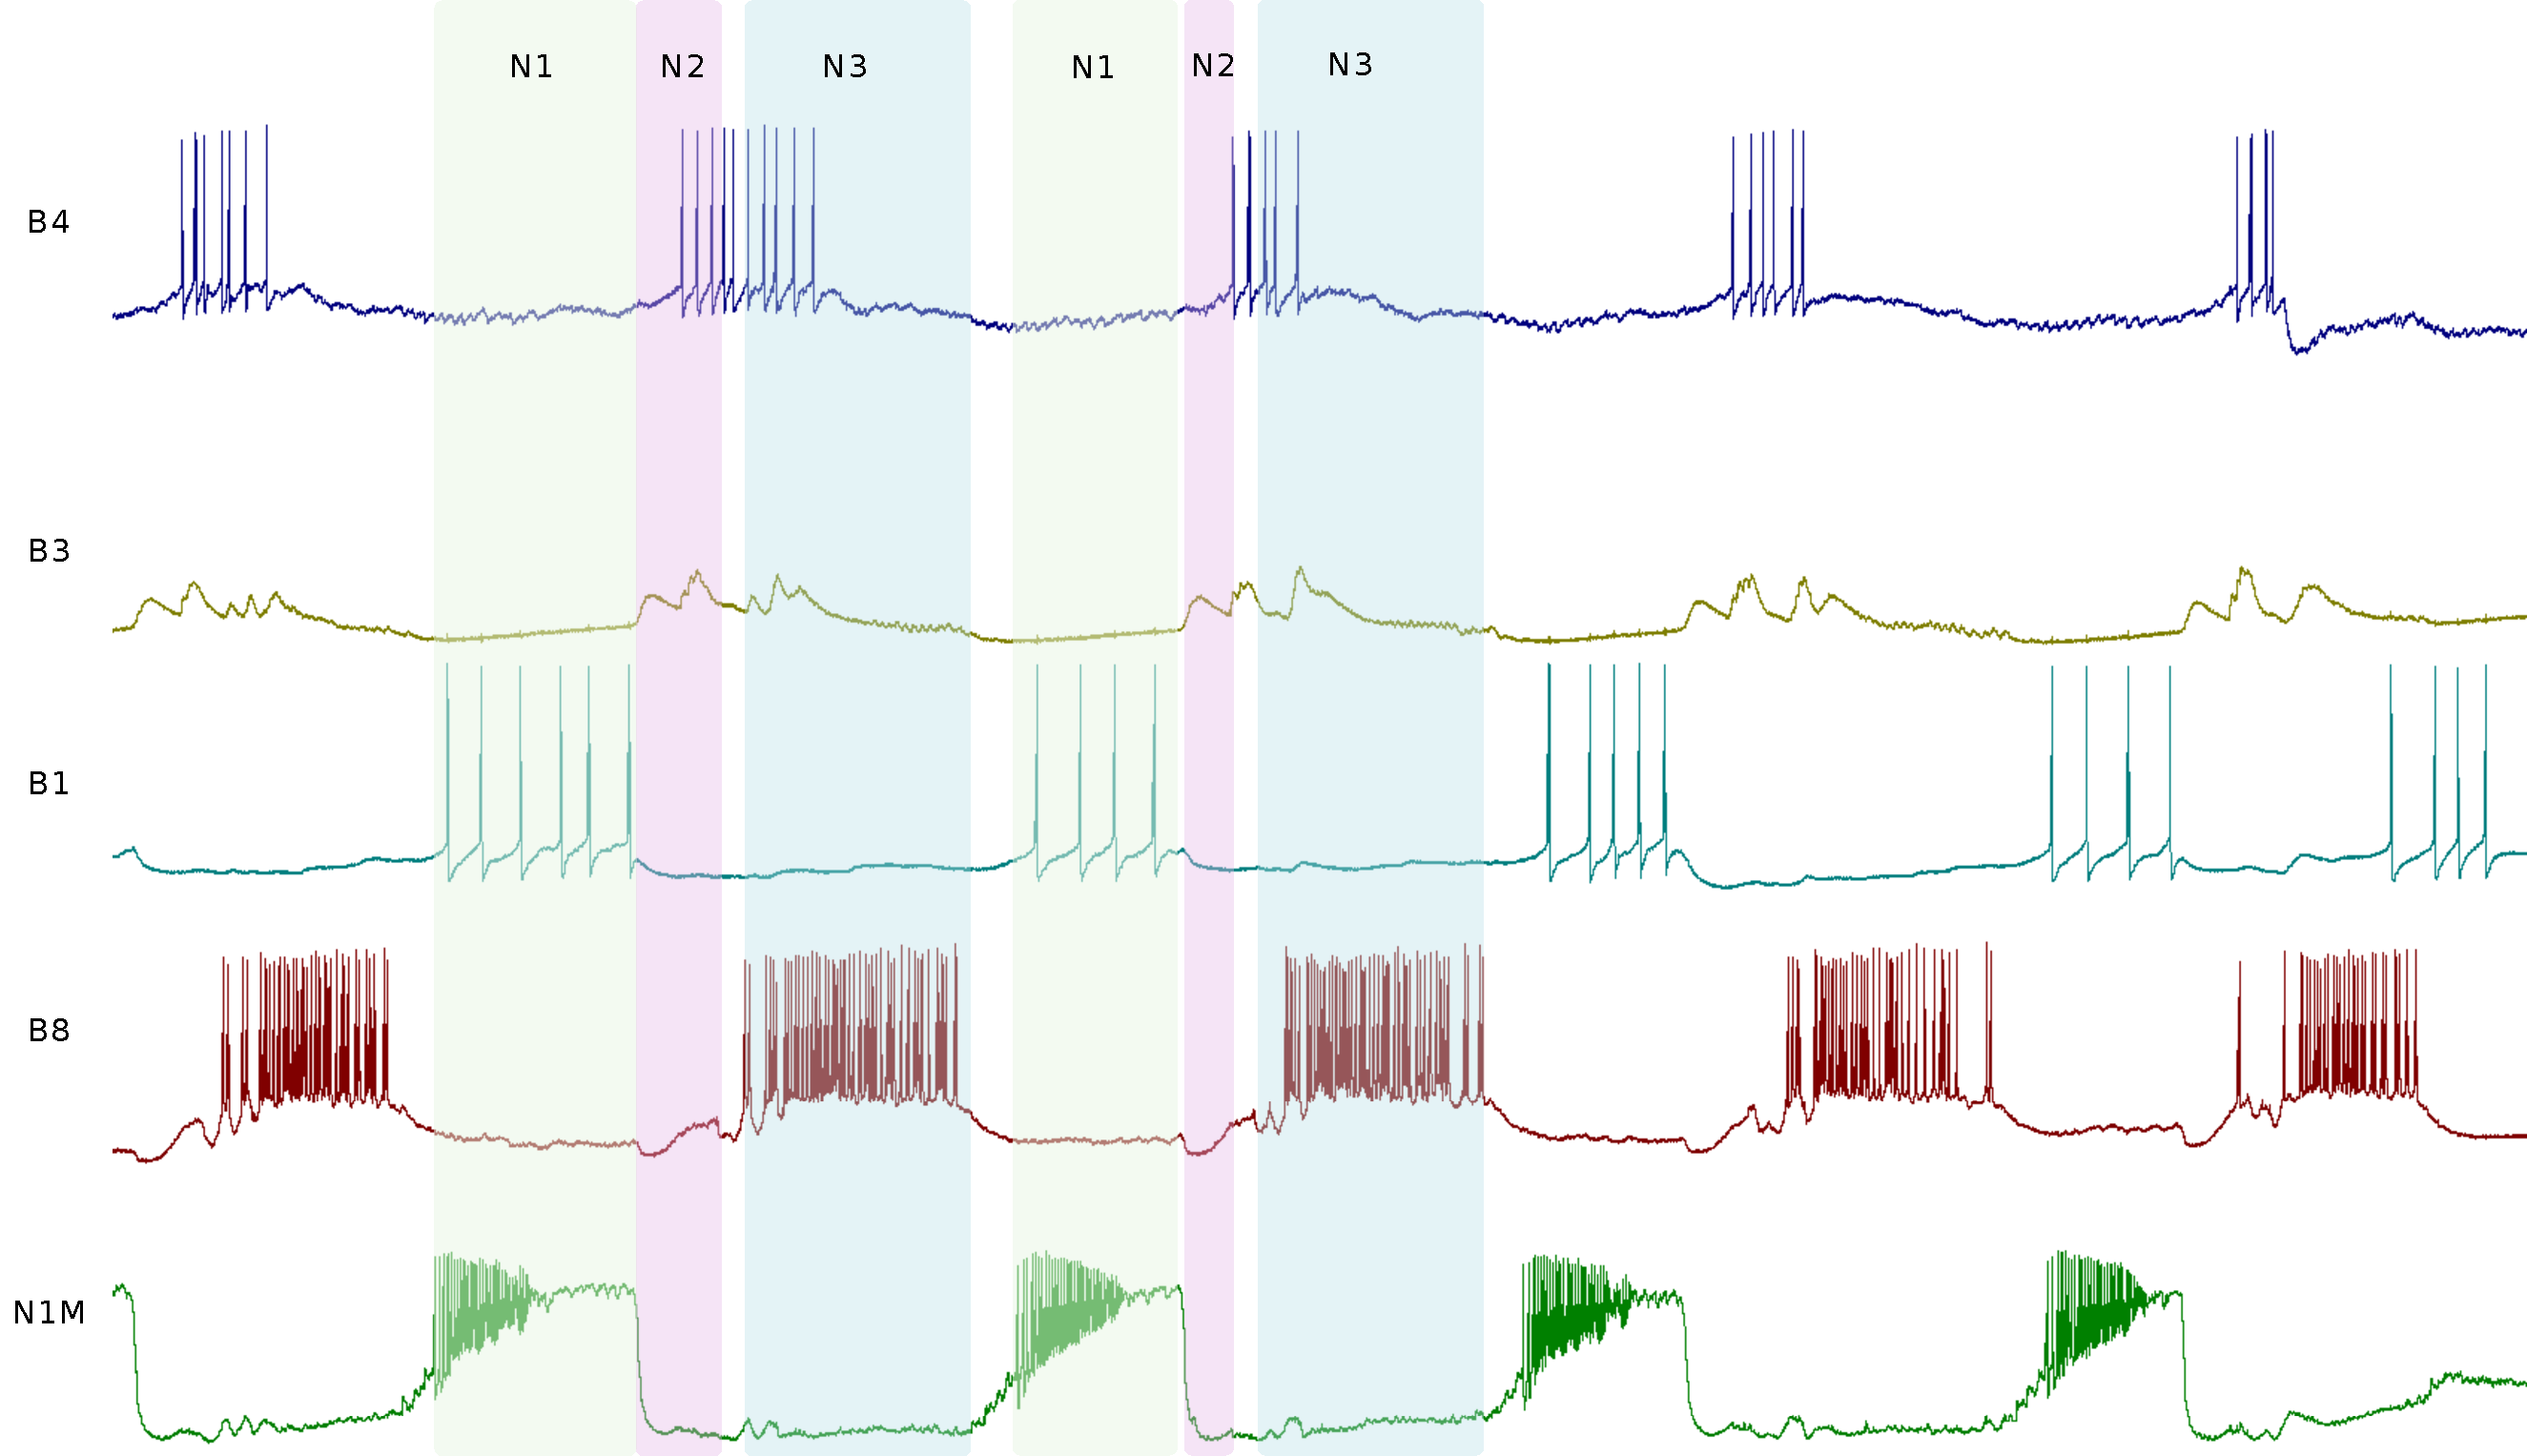
\includegraphics[width=0.9\textwidth]{img/invariants/example_phases_1.pdf}
	\end{minipage}
	\vspace{20pt}
	\begin{minipage}[b]{\textwidth}
		\makebox[0pt][l]{\hspace*{-130pt}\text{b)}}\\
		\centering
		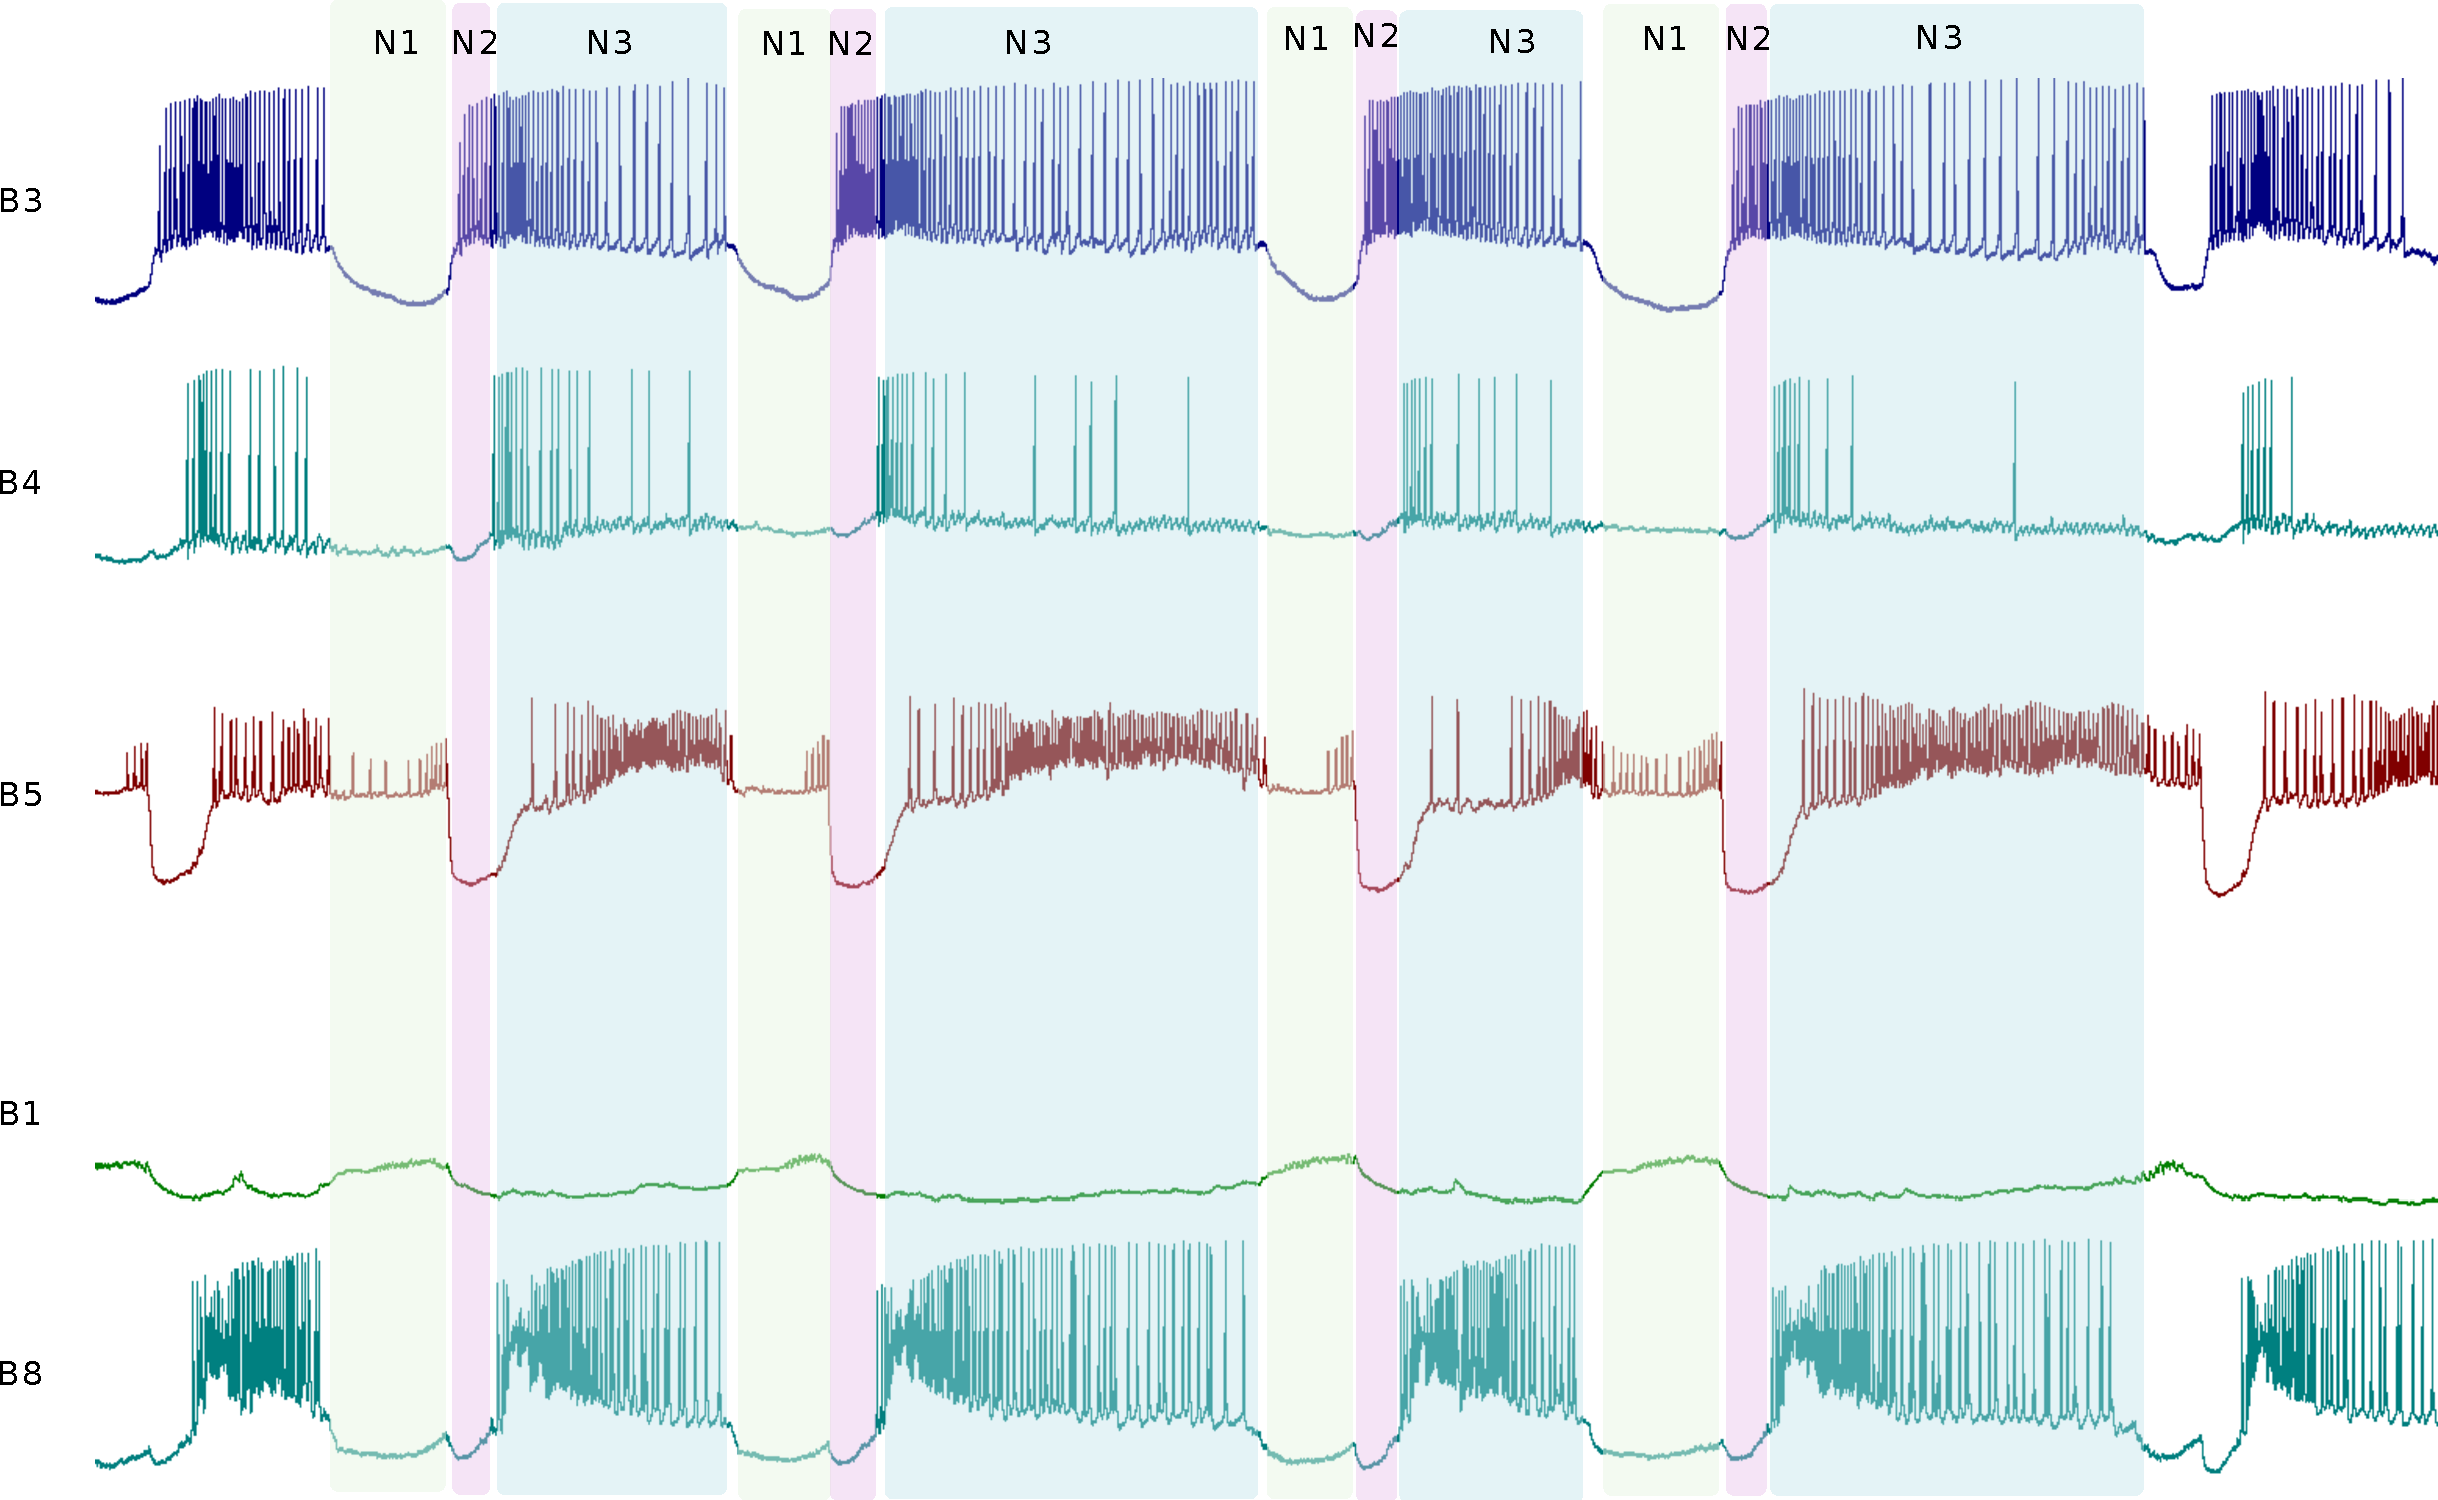
\includegraphics[width=0.9\textwidth]{img/invariants/example_phases_2.pdf}
	\end{minipage}
	\caption{Delimitation of phases in the feeding CPG of \textit{Lymnaea stagnalis} based on different recordings. Panel a) intracellular recordings for motoneurons B4,B3,B1 and B8 and the interneuron N1M. Phases are delimited by N1M and B1, that have the same activation time for phase N1, the inhibition of N1M and the start of the depolarization in B8 for phase N2 and the first and last spike of burst B8 for phase N3. Panel b) intracellular recordings for motoneurons B3,B4,B5, B1 and B8. Phases are delimited by B1 depolarization for phase N1, the strong inhibition of B5 for phase N2 and the fisrt and last spike of burst B8 for phase N3.}
	\label{fig:example lymnaea phases recording}
\end{figure}

Another key point in the study of the feeding CPG of \textit{L. stagnalis} is that the generation of the rhythm is a combined action of different cells \cite{benjamin_distributed_2012}, not only interneurons but also motoneurons have a role in the activation \parencite{staras_pattern-generating_1998} and modulatory neurons in the buccal and cerebral ganglia are involved in the rhythm. All these factors affect the rhythm and thus the neuronal sequential activation and how variability is distributed among the different intervals cycle by cycle. Also, not all the neurons are involved every time the rhythm is active, and that gives also information about the different contexts in which the rhythm is taking part. For example, the rhythm can be activated by the presence of food or sucrose stimulation, in which case the animal needs to initiate the activity and ingest food, the rhythm is started by the stimulation of the lip nerve that also stimulates N1M. Also, even at the absence of food but when the animal is hungry, the CPG can be activated, in this case with a strong role of N3t as modulator. The modulation of the rhythm is also a key aspect and modulatory neurons as SO or CV1a control the rhythm after its initiation, showed to have distinct alternative roles in the activity \parencite{kemenes_multiple_2001}. 

\begin{figure}[bth!]
	\centering
	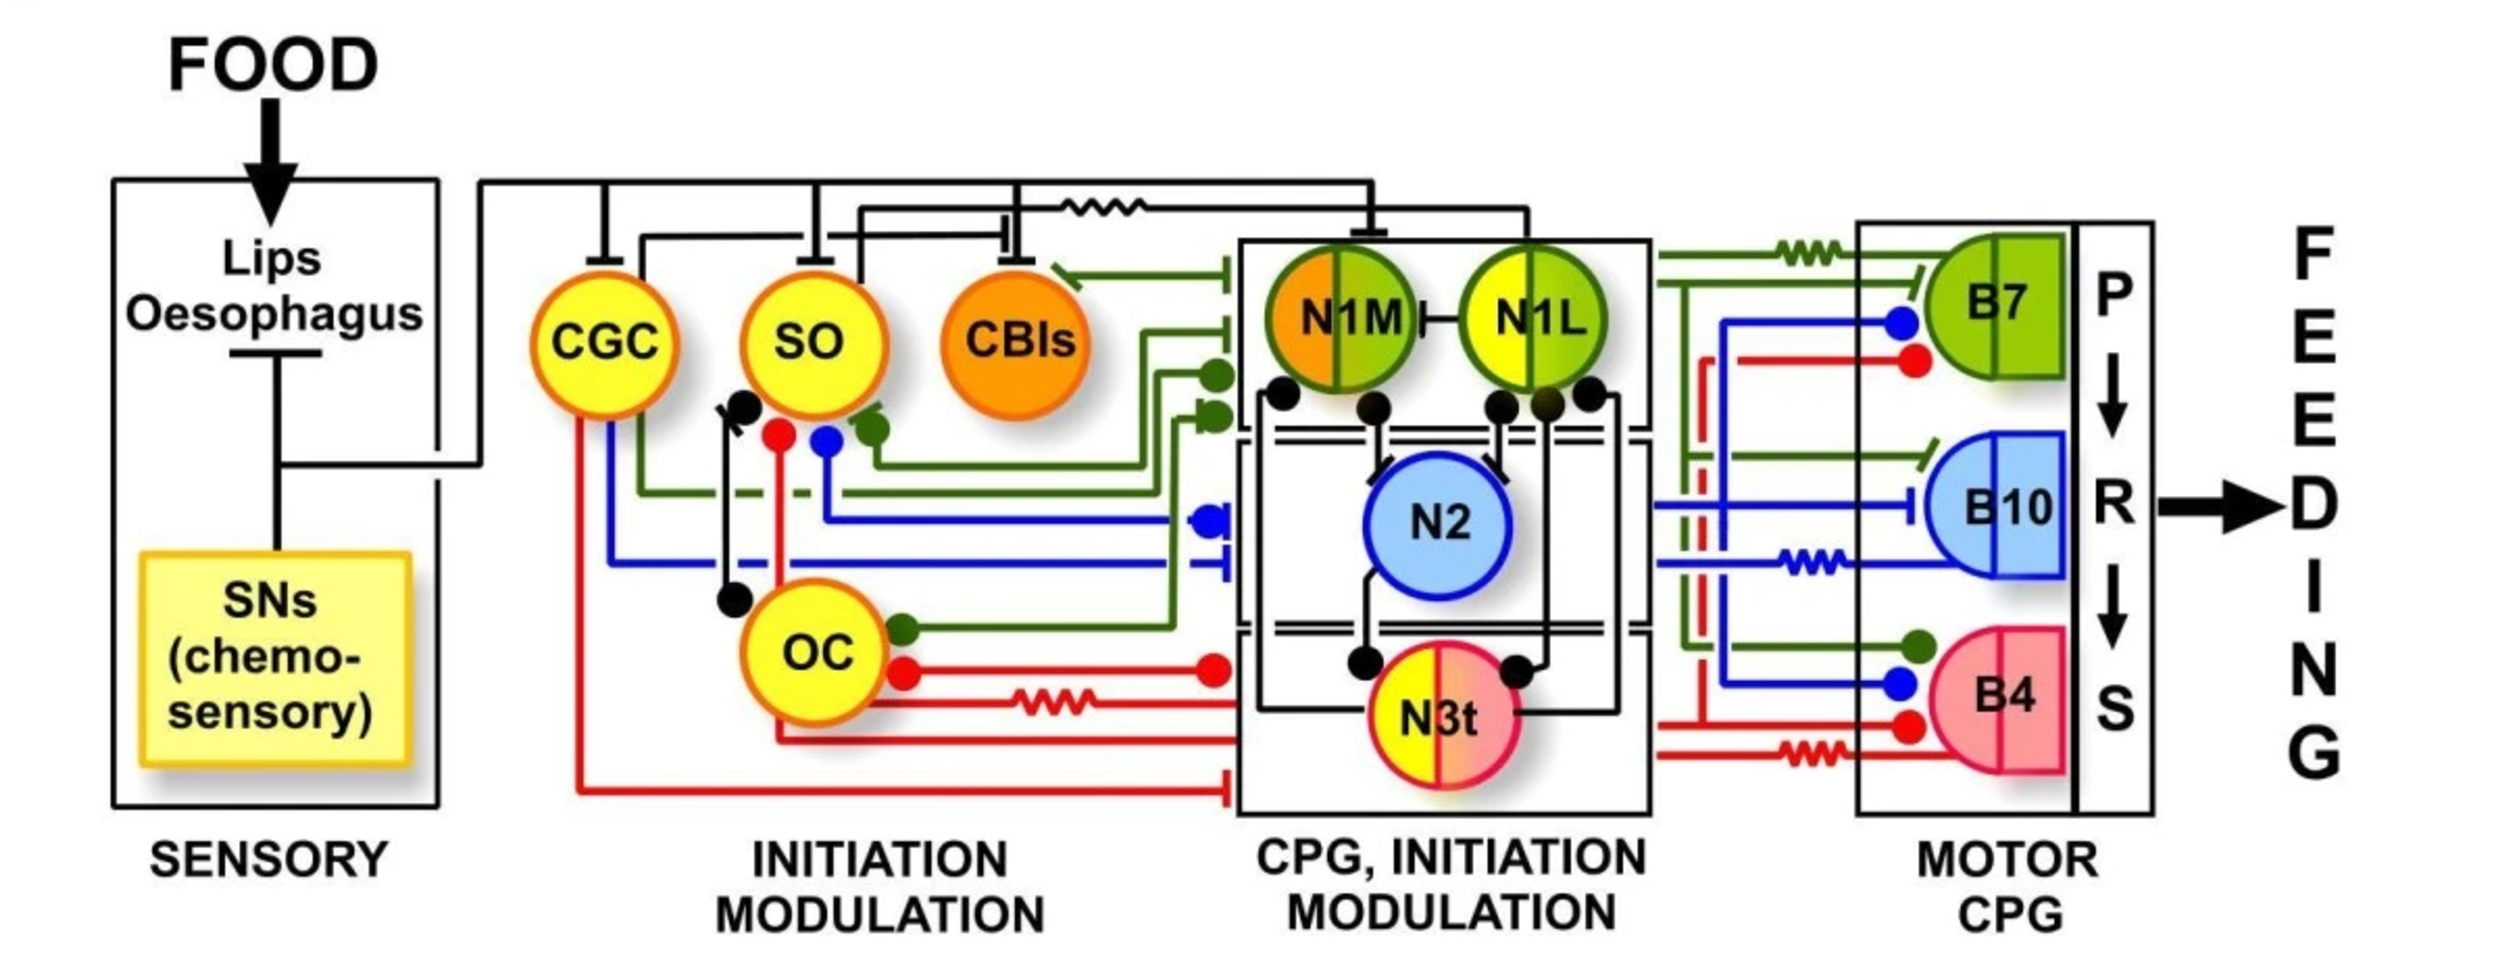
\includegraphics[width=\textwidth]{img/invariants/distributed_benjamin_2012.pdf}
	\caption{Representation of the distributed system of the feeding CPG. Dots indicate inhibitory chemical synapses, bars excitatory chemical synapses and resistor symbols electrotonic (electrical) synapses. Colors indicate the function of the neuron classified in modulatory or initiator (orange and yellow, respectively) and the three phases protraction, rasp and swallow (green, blue and red, respectively). From left to right food detection represented by Lips that stimulate CGC, SO CBIs and N1M neurons and initiate the rhythm. The ongoing activity is then modulated by those neurons but also by OC neurons and N1 and N3t neuron. Some examples of motor neurons are represented on the right side of the panel, associated to each feeding phase. This figure was adapted from Panel C from Figure 1 in \cite{benjamin_distributed_2012} (work under license \href{http://creativecommons.org/licenses/by/2.0}{Creative Commons Attribution})}
	%	Synaptic connectivity and functions of neurons in the feeding circuit. Modulatory function is indicated by yellow and initiating function by orange. CPG interneurons and motoneurons active during the three phases of the feeding rhythm are indicated by green (P = protraction), blue (R = rasp) and red (S = swallow). Neurons labeled with two colors have two functions. Dots indicate inhibitory chemical synapses, bars excitatory chemical synapses and resistor symbols electrotonic (electrical) synapses. This figure emphasizes the point that many of the neurons have more than function in the feeding network. See Abbreviations for all definitions of neuron types.
	\label{fig:feeding distribution}%
\end{figure}

%Benjamin2012    One of the central controllers of
%spontaneous feeding is the N3t CPG interneuron and
%this cell is involved in mediating the effects of hunger
%and satiety. As was described earlier, the N3ts fire toni-
%cally to inhibit the N1M cells and the rate of this tonic
%activity determines the level of activity in the whole feed-
%ing CPG. By comparing the rates of firing in isolated
%ganglia it was found that the N3t firing frequency was
%higher in satiated compared with starved snails and that
%this was inversely correlated to the frequency of sponta-
%neously fictive feeding cycles [4]. 

%kemenes 2001
%CV1a by modulating motoneuron burst duration and SO by setting the frequency of the ongoing rhythm

In this section we will analyze and describe different examples of experiments for the isolated ganglia with intracellular recordings under: spontaneous activity, SO-driven activity spontaneous and induced, medium lip nerve stimulation induced activity and CV1a-driven induced activity.



\subsection{Invariants in spontaneous activity}
The spontaneous activity here refers to intracellular recordings of the buccal ganglia after the isolation of the CNS with no chemical or electrical induced stimulation. In that case, since the CPG is able to maintain the activity in an autonomous manner, it keeps the motor activity as if the CNS was not isolated. In this case, although the characterization of the sequential dynamical invariants can be done, their possible functionality association is more complicated, since the context of the movement origin is lost. The study of these sequential restriction in artificial stimulation context can help classify this spontaneous activity, even when the rest of the system is not available. 

Here we analyze three examples of the spontaneous activity, 

\paragraph{Spontaneous Activity Example 1}
N1 phase was analyzed from B1 activity (bursting and depolarization); N2 phase was analyzed from B5 hyperpolarization, which has a strong inhibition from N2v; N3 phase was analyzed from the bursting activity of B8, that replicates the N3t duration. 

\begin{figure}[htbp]
	\centering
	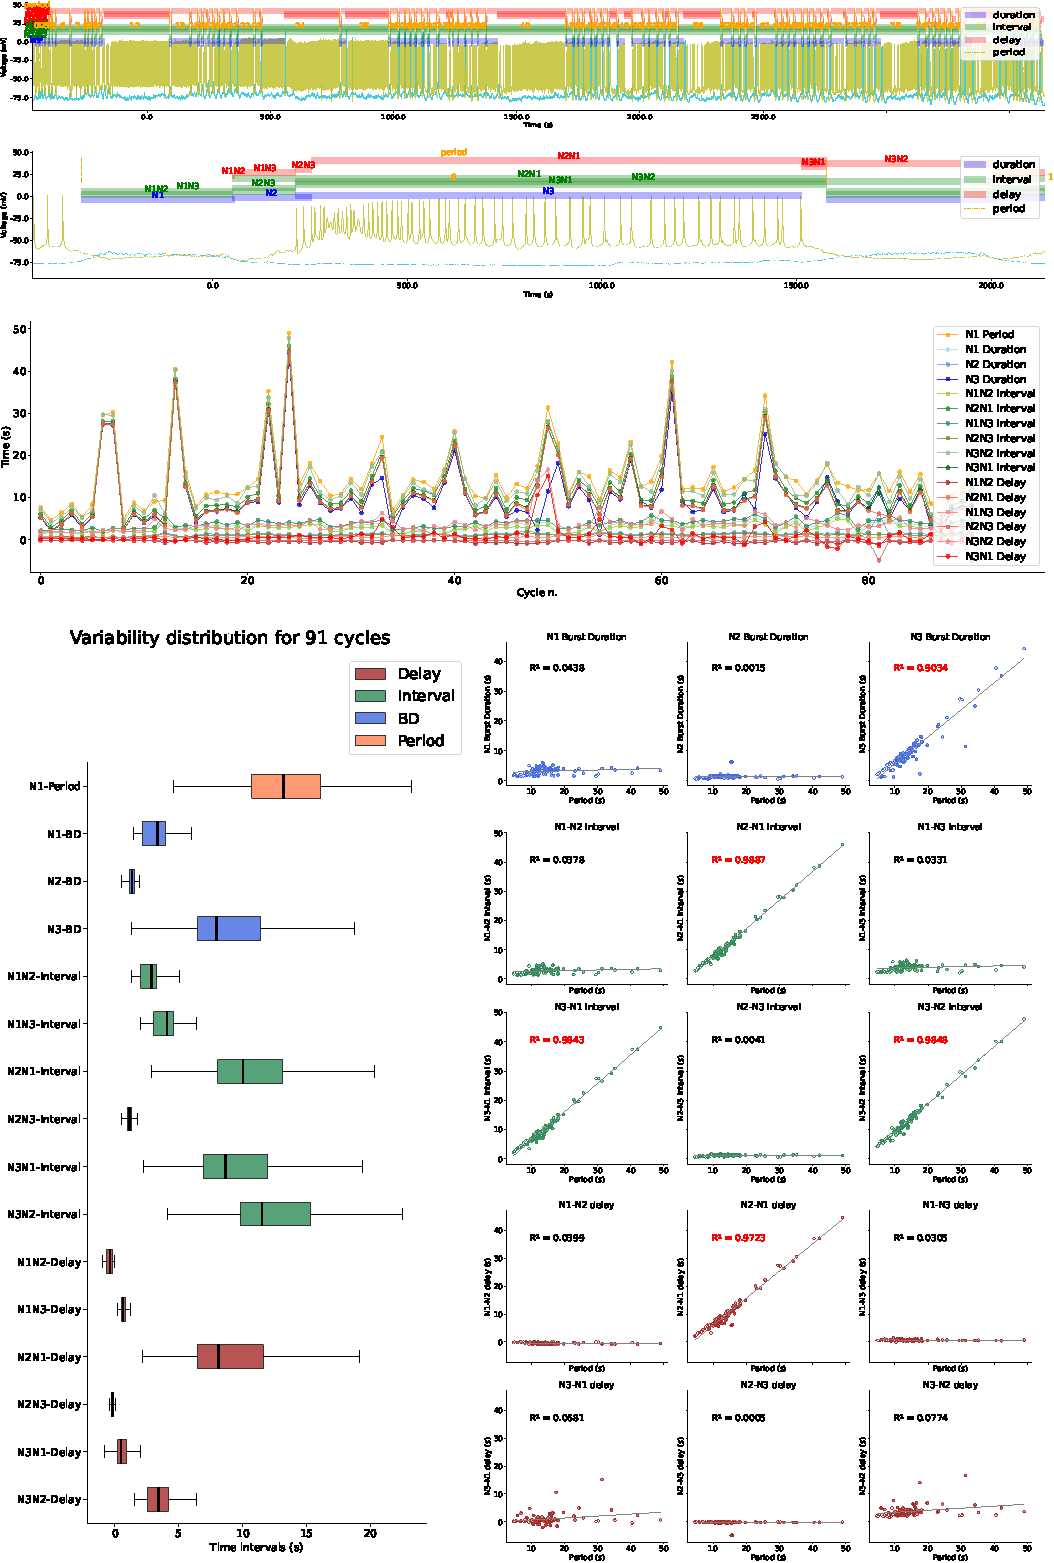
\includegraphics[width=0.9\textwidth]{./img/invariants/data/SUSSEX/prep2/images/3phases/panel_with_intervals.pdf}
	\caption{\textbf{Spontaneous case 1}: Panel of intervals distribution and dynamical invariants for the three phases in the CPG for spontaneous activity.}
	\label{fig:prep2 invariants}
\end{figure}
%
%\begin{figure}[htbp]
%	\centering
%	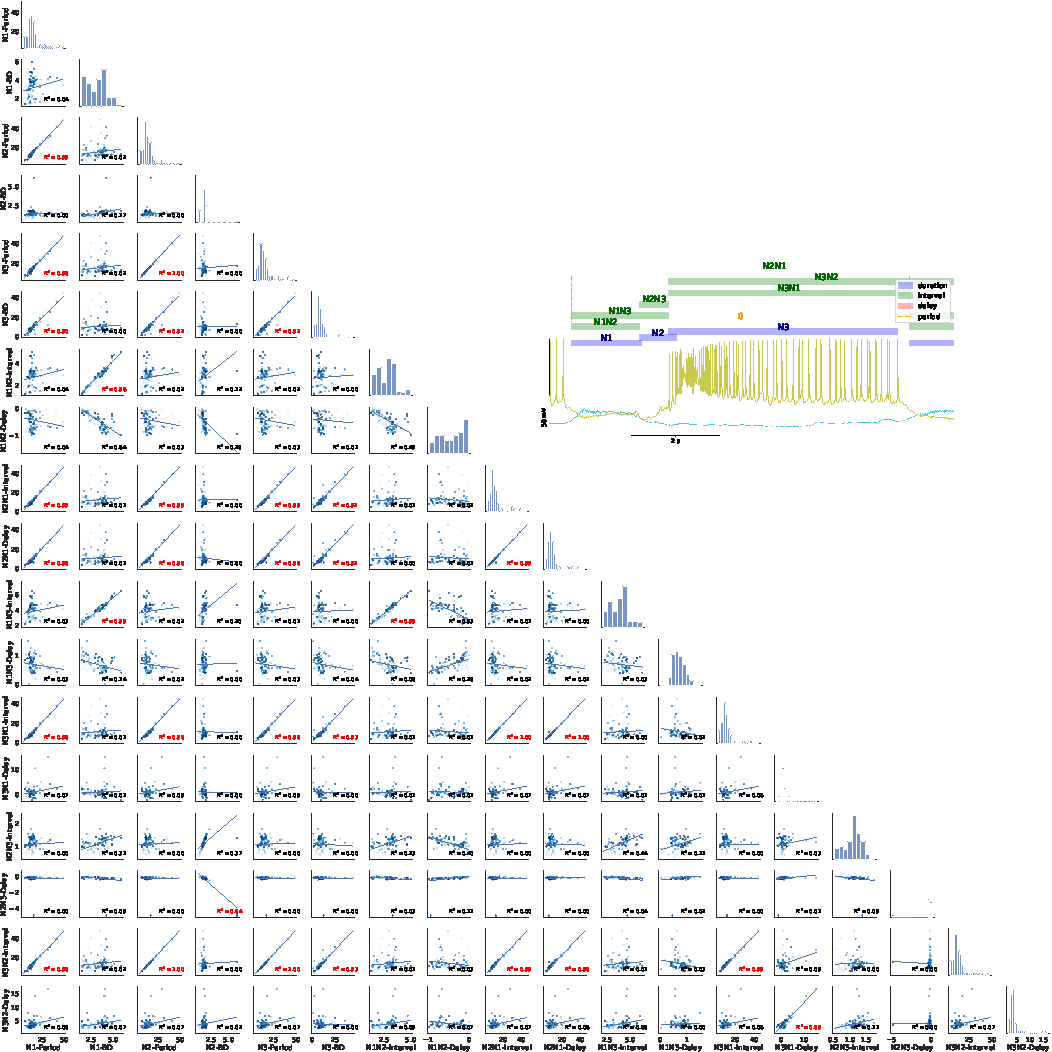
\includegraphics[width=\textwidth]{./img/invariants/data/SUSSEX/prep2/images/3phases/panel_with_pairplot.pdf}
%	\caption{\textbf{Spontaneous case 1}: Panel of intervals distribution and dynamical invariants for the three phases in the CPG for spontaneous activity.}
%	\label{fig:prep2 pairplot invariants}
%\end{figure}


%\begin{figure}[htbp]
%	\centering
%	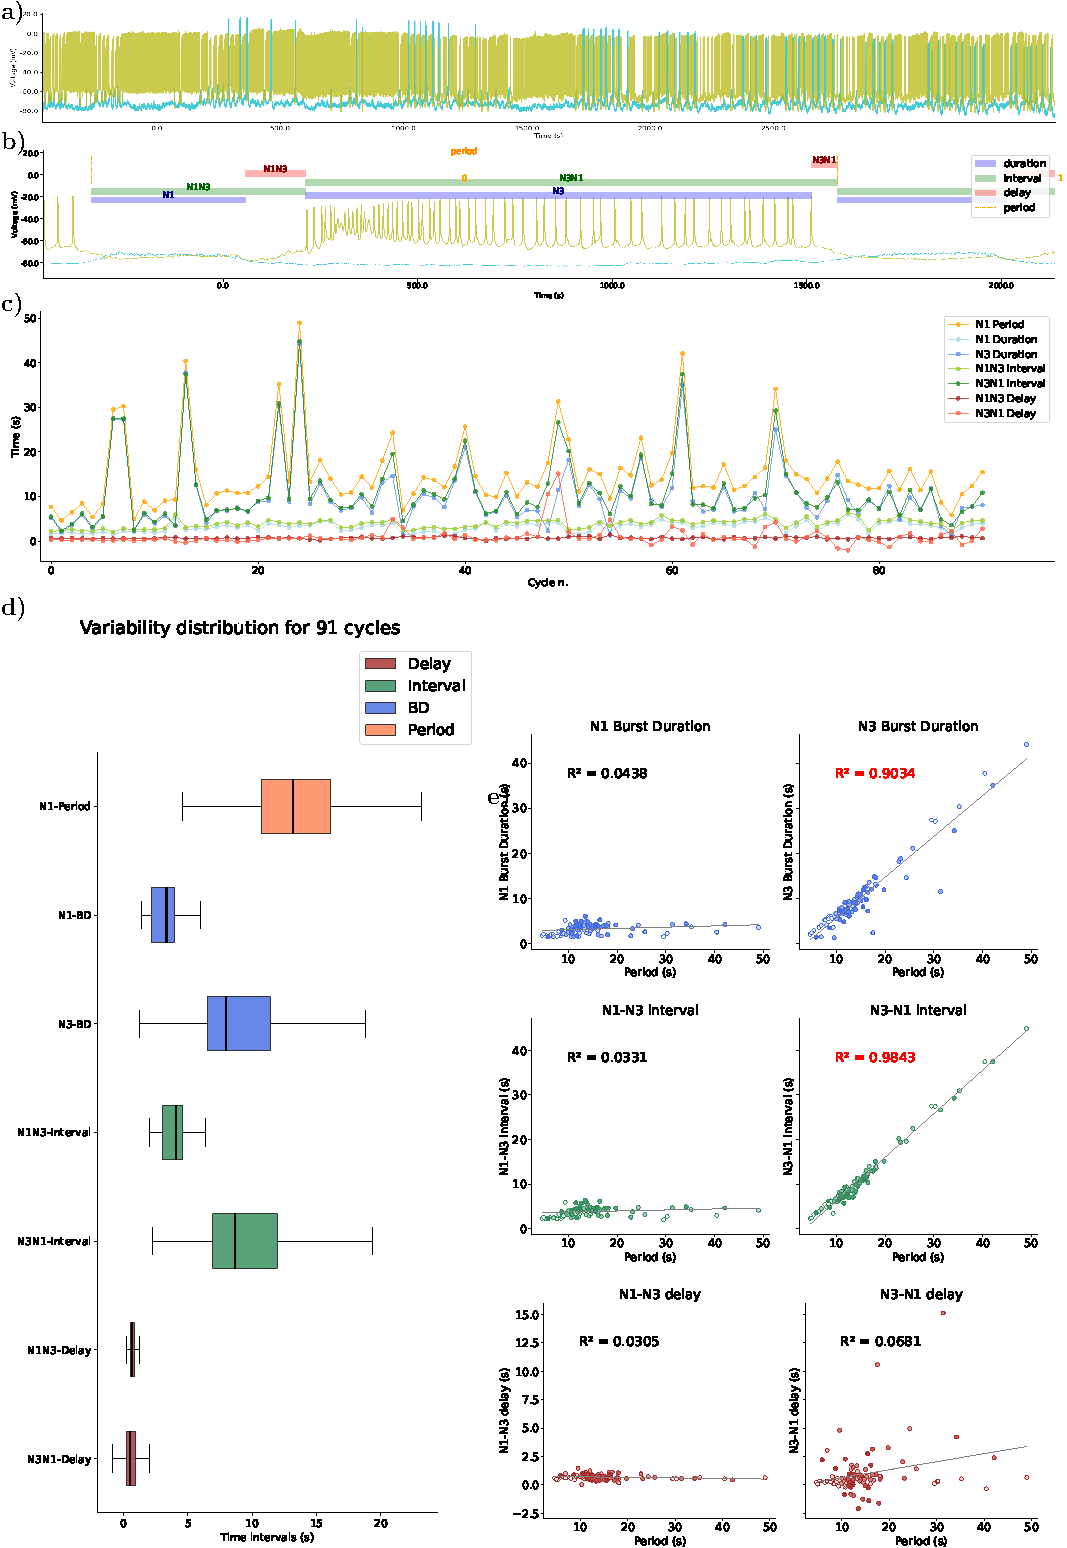
\includegraphics[width=0.9\textwidth]{./img/invariants/data/SUSSEX/prep2/images/2phases/panel_with_intervals.pdf}
%	\caption{\textbf{Spontaneous case2}: Panel of intervals distribution and dynamical invariants for two phases in the CPG for spontaneous activity.}
%	\label{fig:prep2 2phase invariants}
%\end{figure}
%
%\begin{figure}[htbp]
%\centering
%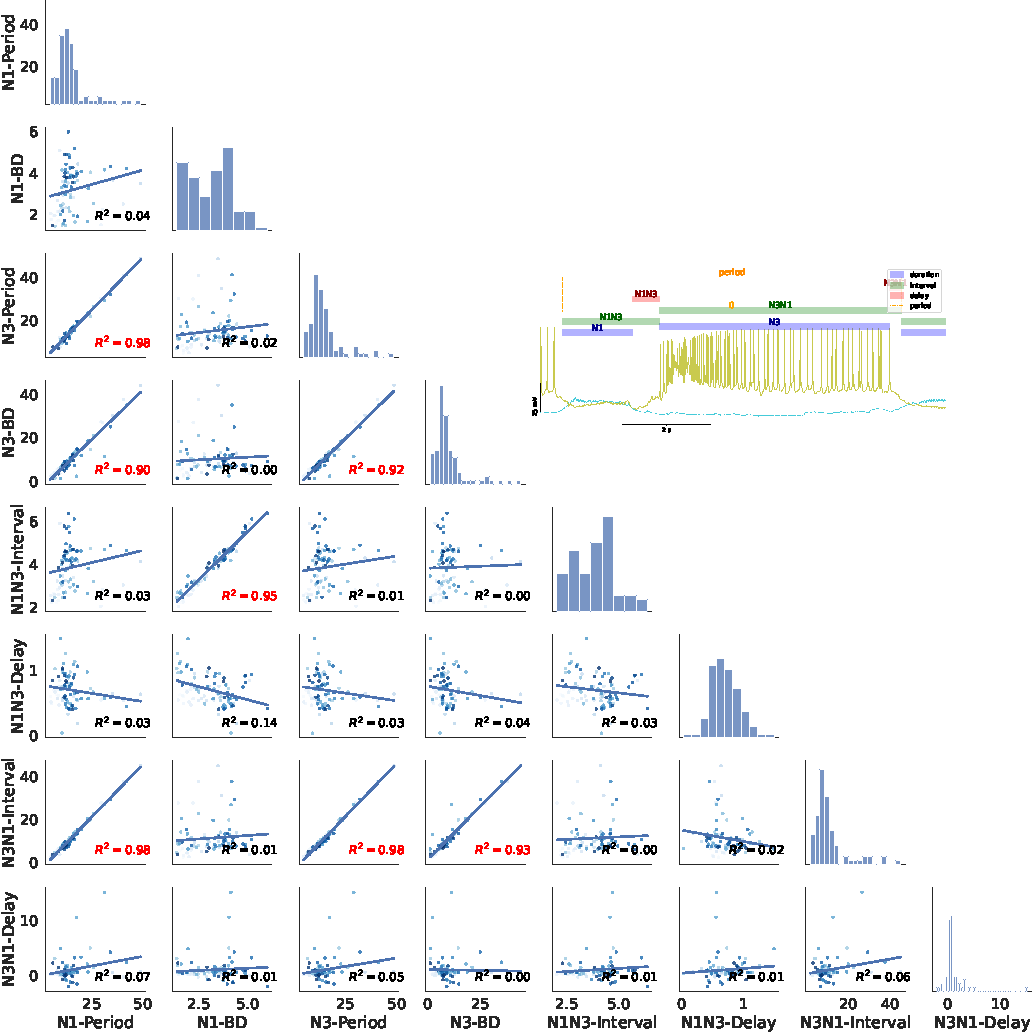
\includegraphics[width=0.9\textwidth]{./img/invariants/data/SUSSEX/prep2/images/2phases/panel_with_pairplot.pdf}
%\caption{\textbf{Spontaneous case2}: Panel of intervals distribution and dynamical invariants for two phases in the CPG for spontaneous activity.}
%\label{fig:prep2 2phase invariants pairplot}
%\end{figure}

\paragraph{Spontaneous Activity Example 2}
N1 phase was analyzed from B1 activity (bursting and depolarization); N2 phase was analyzed from B1 hyperpolarization, which has a strong inhibition from N2v; N3 phase was analyzed from the bursting activity of B8, that replicates the N3t duration. 
Since the reference for N2 here coincides with N1 reference, we display here only the intervals corresponding to N1 and N3 phases, since the intervals that correspond to 3 phases, such as N1-N2 delay or N2-N3 delay, either are already represented in the defined intervals or have a duration close to 0 ms.

%\begin{figure}[htbp]
%	\centering
%	\includegraphics[width=0.9\textwidth]{./img/invariants/data/SUSSEX/prep3/images/phases/panel_with_intervals.pdf}
%	\caption{\textbf{Spontaneous case 2}: Panel of intervals distribution and dynamical invariants for two phases in the CPG for spontaneous activity.}
%	\label{fig:prep3 2phases invariants}
%\end{figure}

%\begin{figure}[htbp]
%	\centering
%	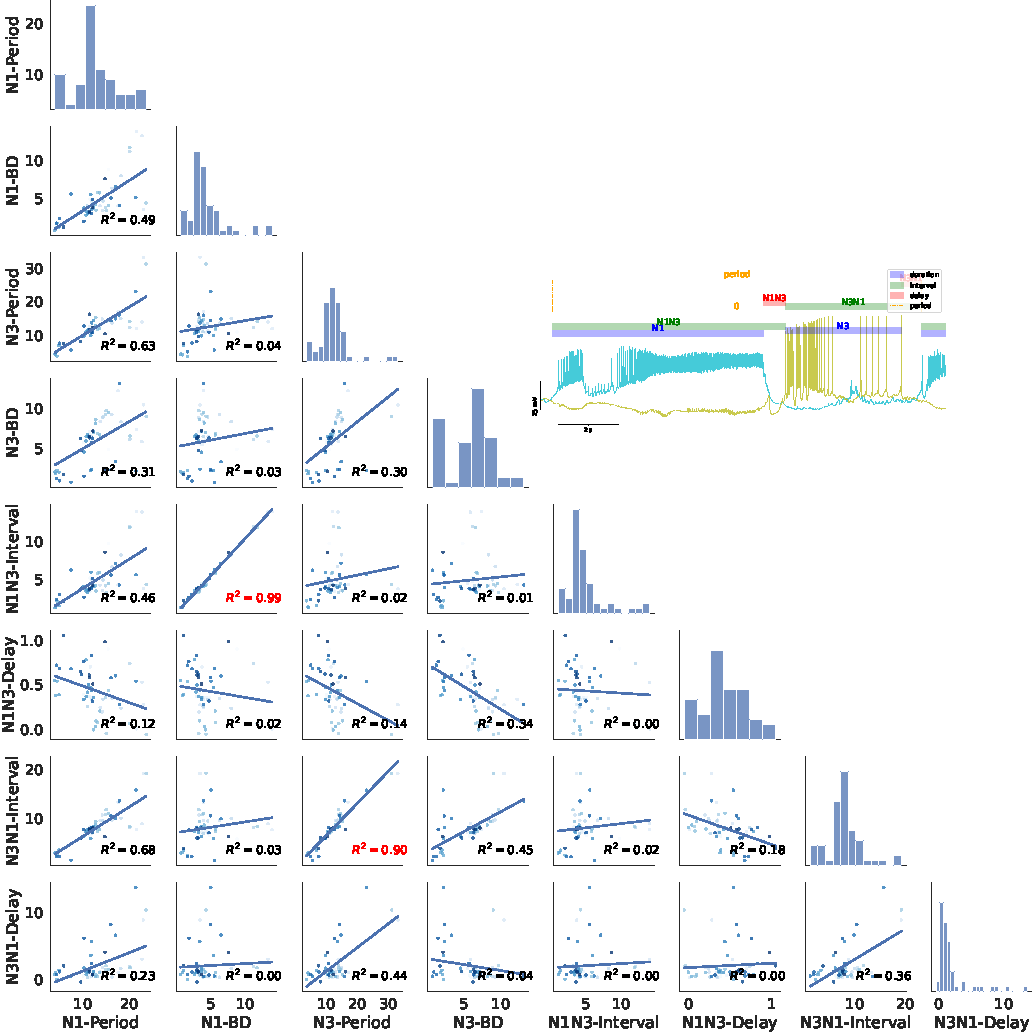
\includegraphics[width=0.9\textwidth]{./img/invariants/data/SUSSEX/prep3/images/2phases/panel_with_pairplot.pdf}
%	\caption{\textbf{Spontaneous case 2}: Panel of intervals distribution and dynamical invariants for two phases in the CPG for spontaneous activity.}
%	\label{fig:prep3 2phases invariants pairplot}
%\end{figure}

\begin{figure}[htbp]
	\centering
	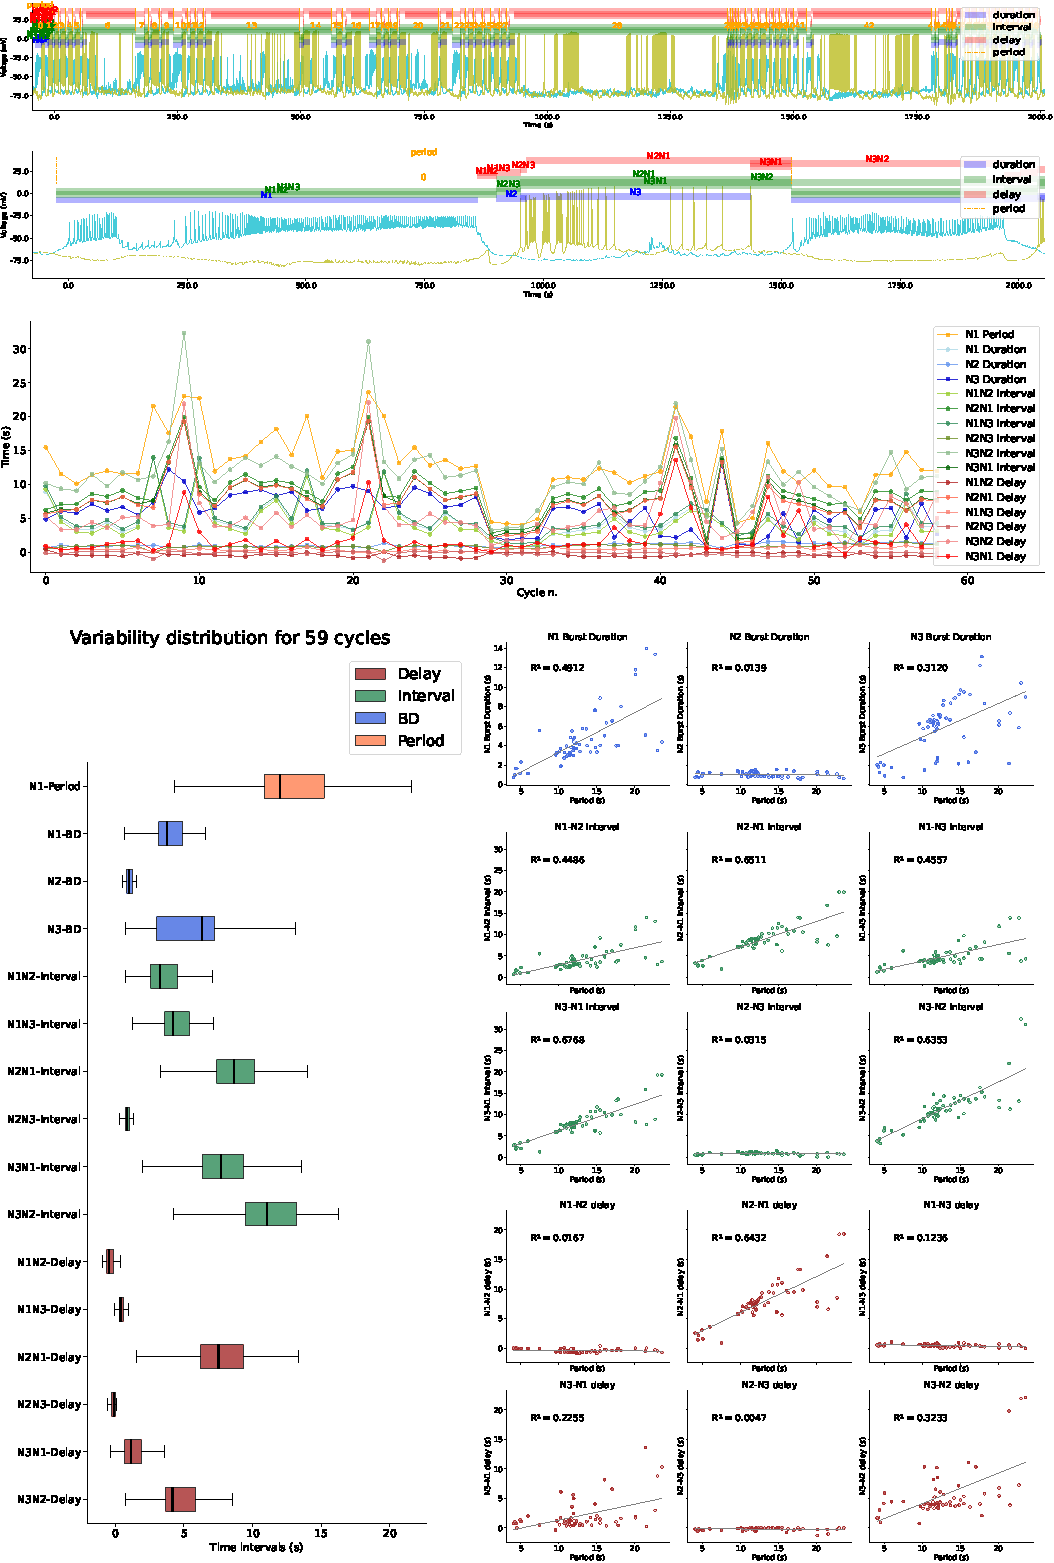
\includegraphics[width=0.9\textwidth]{./img/invariants/data/SUSSEX/prep3/images/3phases/panel_with_intervals.pdf}
	\caption{\textbf{Spontaneous case3}: Panel of intervals distribution and dynamical invariants for the three phases in the CPG for spontaneous activity.}
	\label{fig:prep3 invariants}
\end{figure}
%
%\begin{figure}[htbp]
%	\centering
%	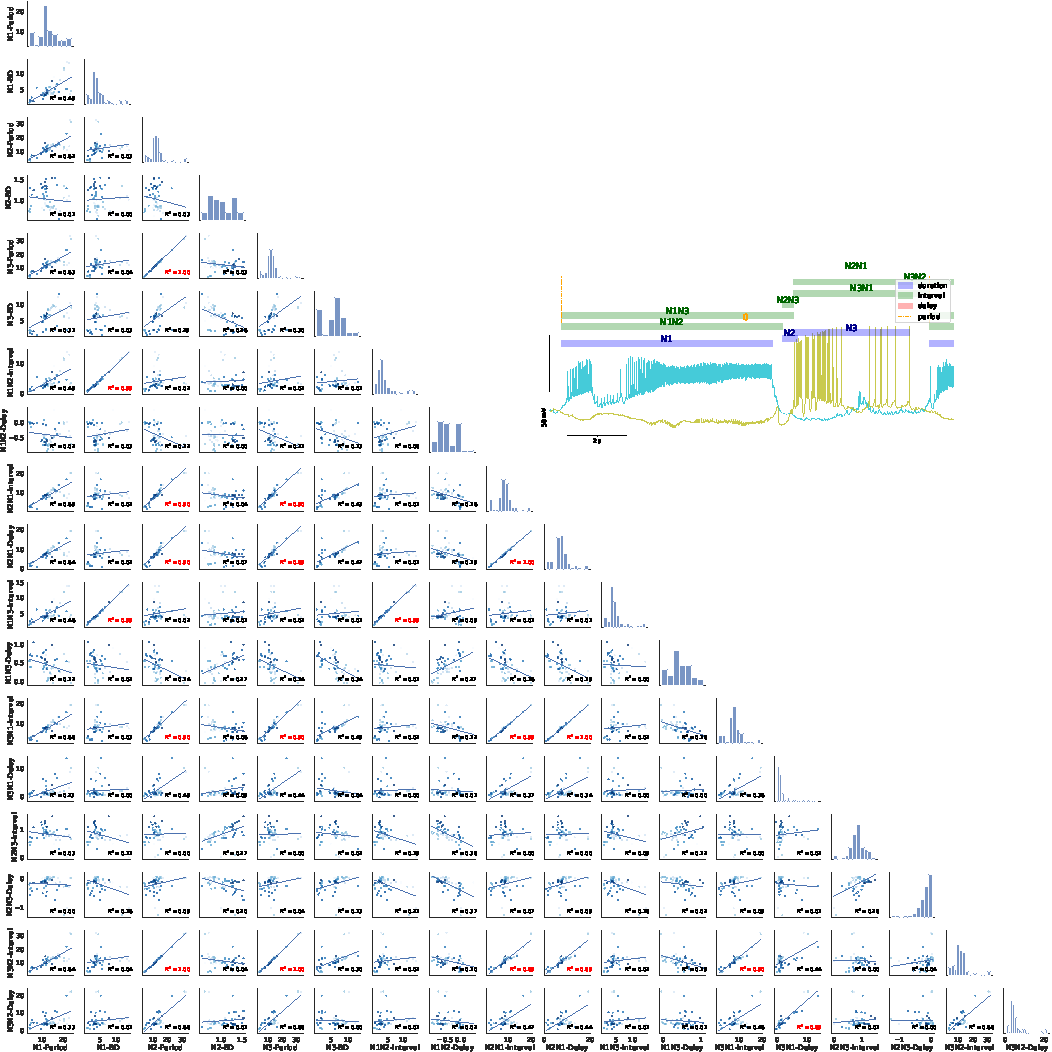
\includegraphics[width=0.9\textwidth]{./img/invariants/data/SUSSEX/prep3/images/3phases/panel_with_pairplot.pdf}
%	\caption{\textbf{Spontaneous case3}: Panel of intervals distribution and dynamical invariants for the three phases in the CPG for spontaneous activity.}
%	\label{fig:prep3 invariants pairplot}
%\end{figure}


\paragraph{Spontaneous Activity Example 3}
N1 phase was analyzed from B1 activity (bursting and depolarization); N2 phase was analyzed from B5 hyperpolarization, which has a strong inhibition from N2v; N3 phase was analyzed from the bursting activity of B8, that replicates the N3t duration. 

\begin{figure}[htbp]
	\centering
	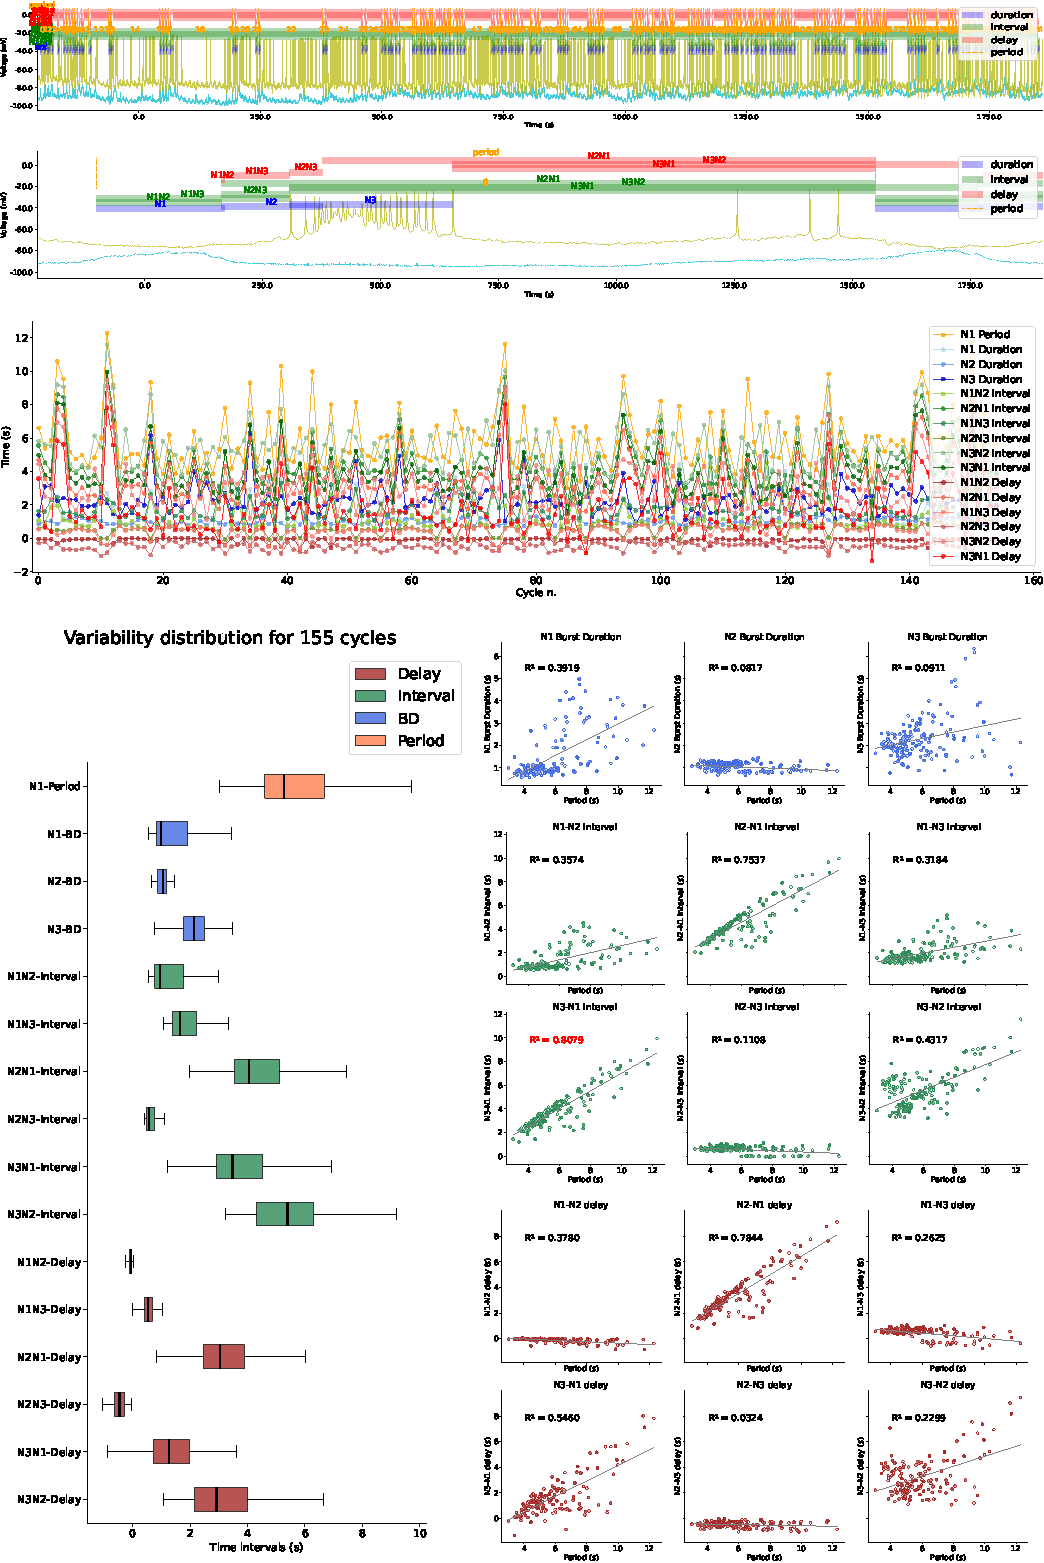
\includegraphics[width=0.9\textwidth]{./img/invariants/data/SUSSEX/prep1/images/3phases/panel_with_intervals.pdf}
	\caption{\textbf{Spontaneous case 3}: Panel of intervals distribution and dynamical invariants for the three phases in the CPG for spontaneous activity.}
	\label{fig:prep1 invariants}
\end{figure}


%\begin{figure}[htbp]
%	\centering
%	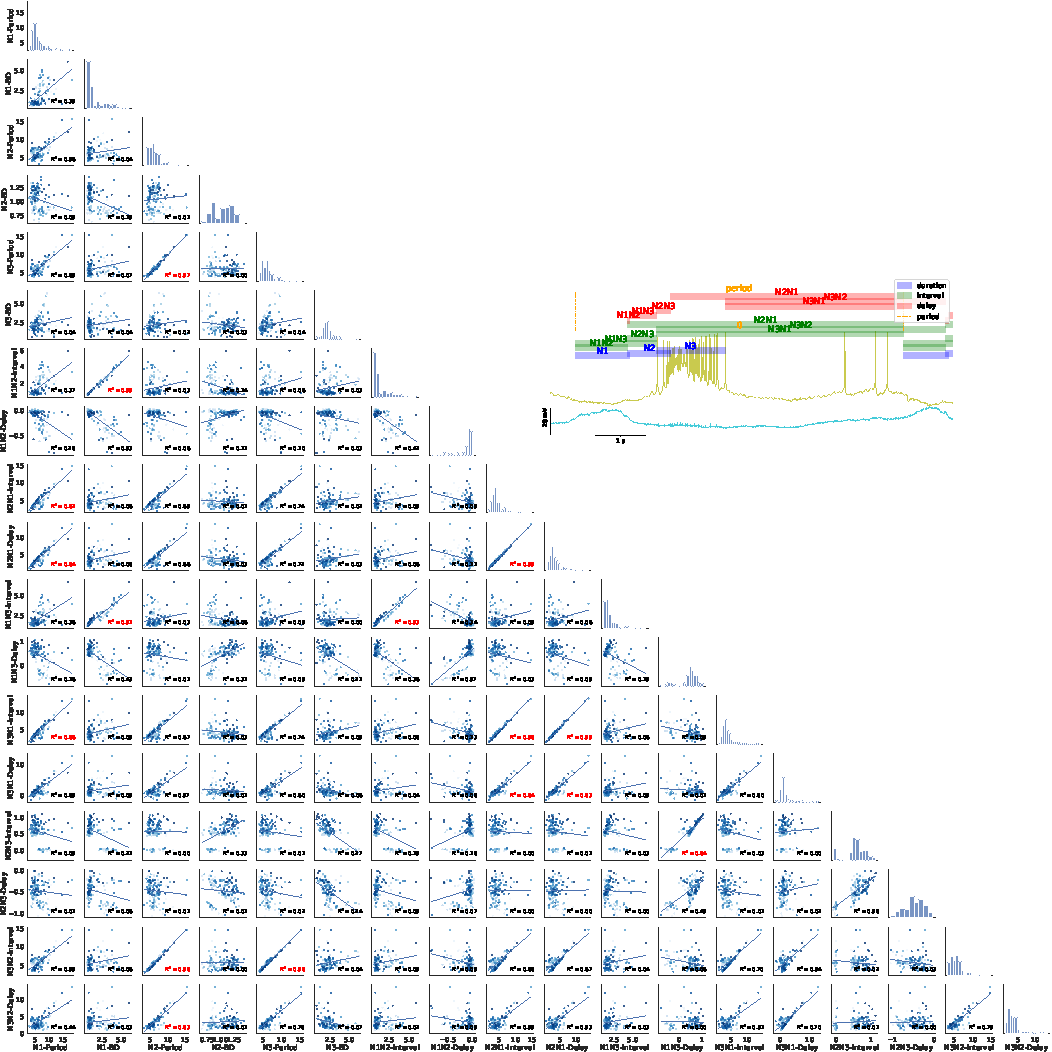
\includegraphics[width=\textwidth]{./img/invariants/data/SUSSEX/prep1/images/3phases/panel_with_pairplot.pdf}
%	\caption{\textbf{Spontaneous case 3}: Panel of intervals distribution and dynamical invariants for the three phases in the CPG for spontaneous activity.}
%	\label{fig:prep1 invariants pairplot}
%\end{figure}

%
%\begin{figure}[htbp]
%	\centering
%	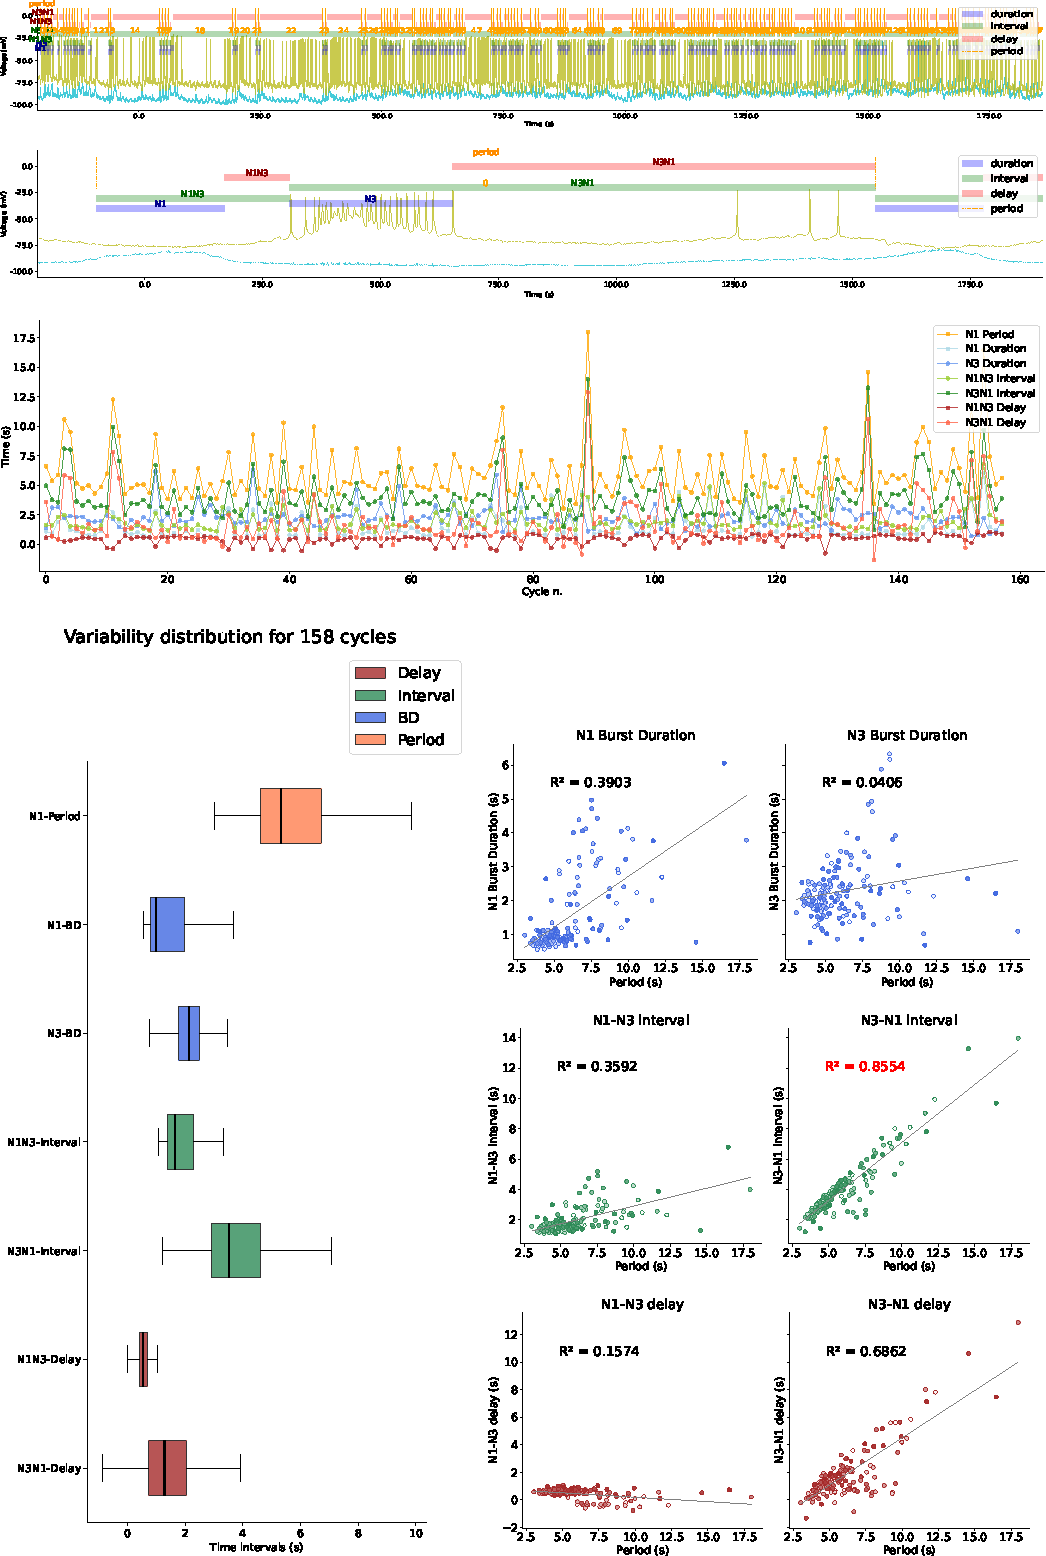
\includegraphics[width=0.9\textwidth]{./img/invariants/data/SUSSEX/prep1/images/2phases/panel_with_intervals.pdf}
%	\caption{\textbf{Spontaneous case1}: Panel of intervals distribution and dynamical invariants for two phases in the CPG for spontaneous activity.}
%	\label{fig:prep1 2 phases invariants}
%\end{figure}
%%
%\begin{figure}[htbp]
%	\centering
%	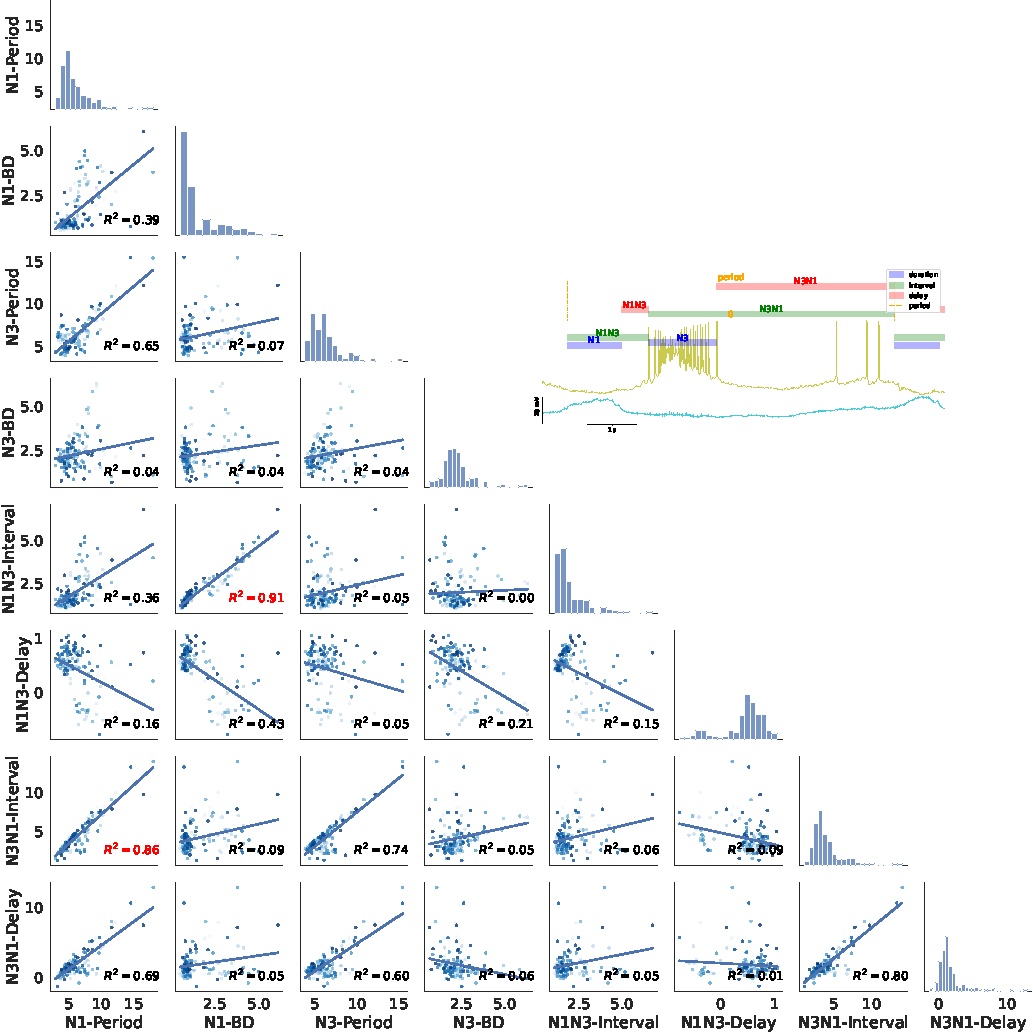
\includegraphics[width=0.9\textwidth]{./img/invariants/data/SUSSEX/prep1/images/2phases/panel_with_pairplot.pdf}
%	\caption{\textbf{Spontaneous case1}: Panel of intervals distribution and dynamical invariants for the two phases in the CPG for spontaneous activity.}
%	\label{fig:prep1 2 phases invariants pairplot}
%\end{figure}


\begin{figure}[htbp]
	\centering
	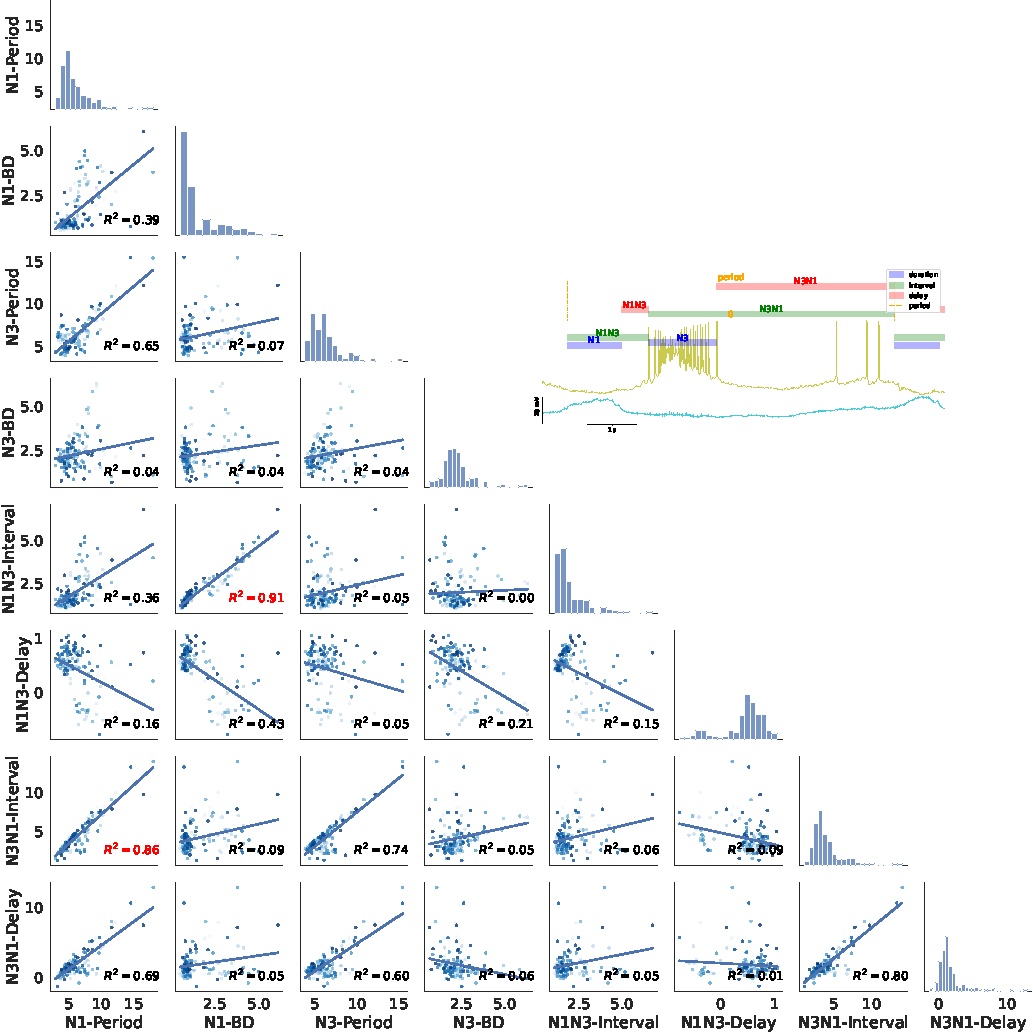
\includegraphics[width=0.48\textwidth]{./img/invariants/data/SUSSEX/prep1/images/2phases/panel_with_pairplot.pdf}
	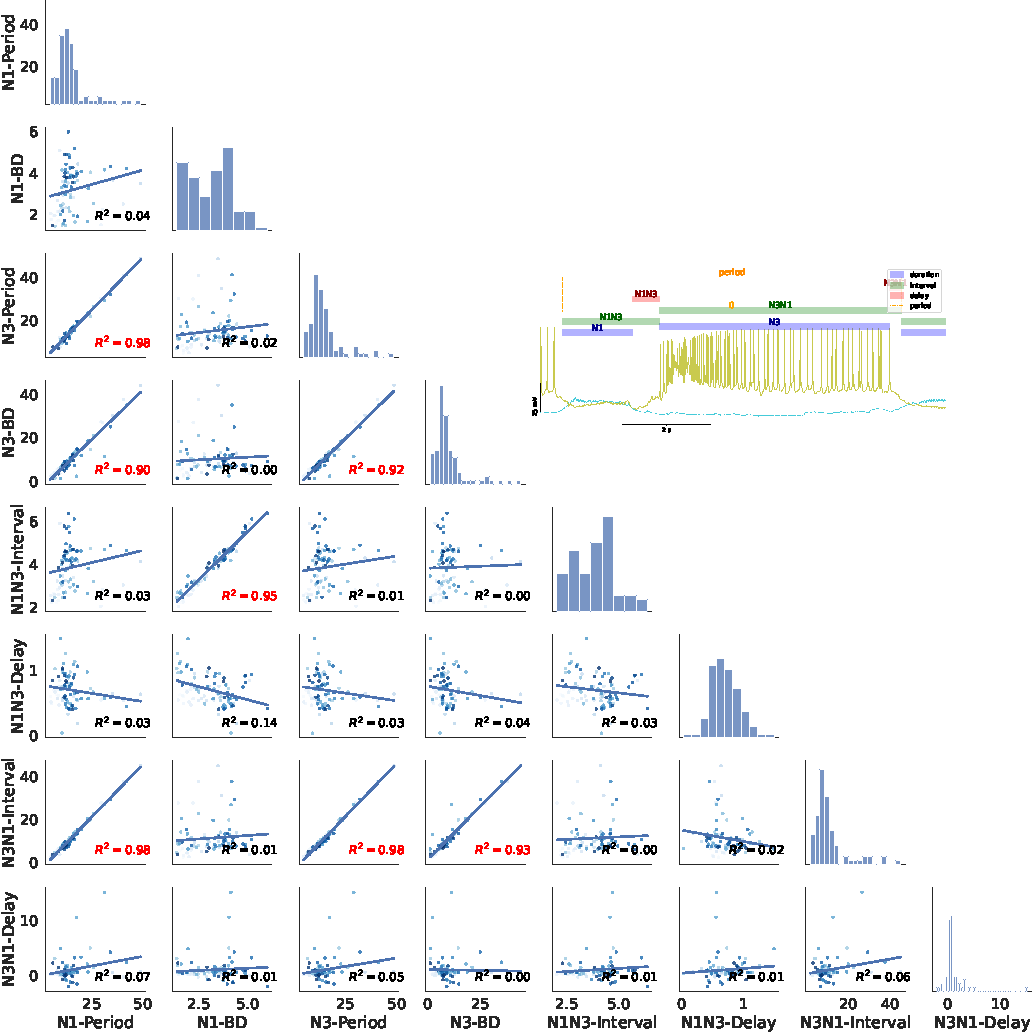
\includegraphics[width=0.48\textwidth]{./img/invariants/data/SUSSEX/prep2/images/2phases/panel_with_pairplot.pdf}
	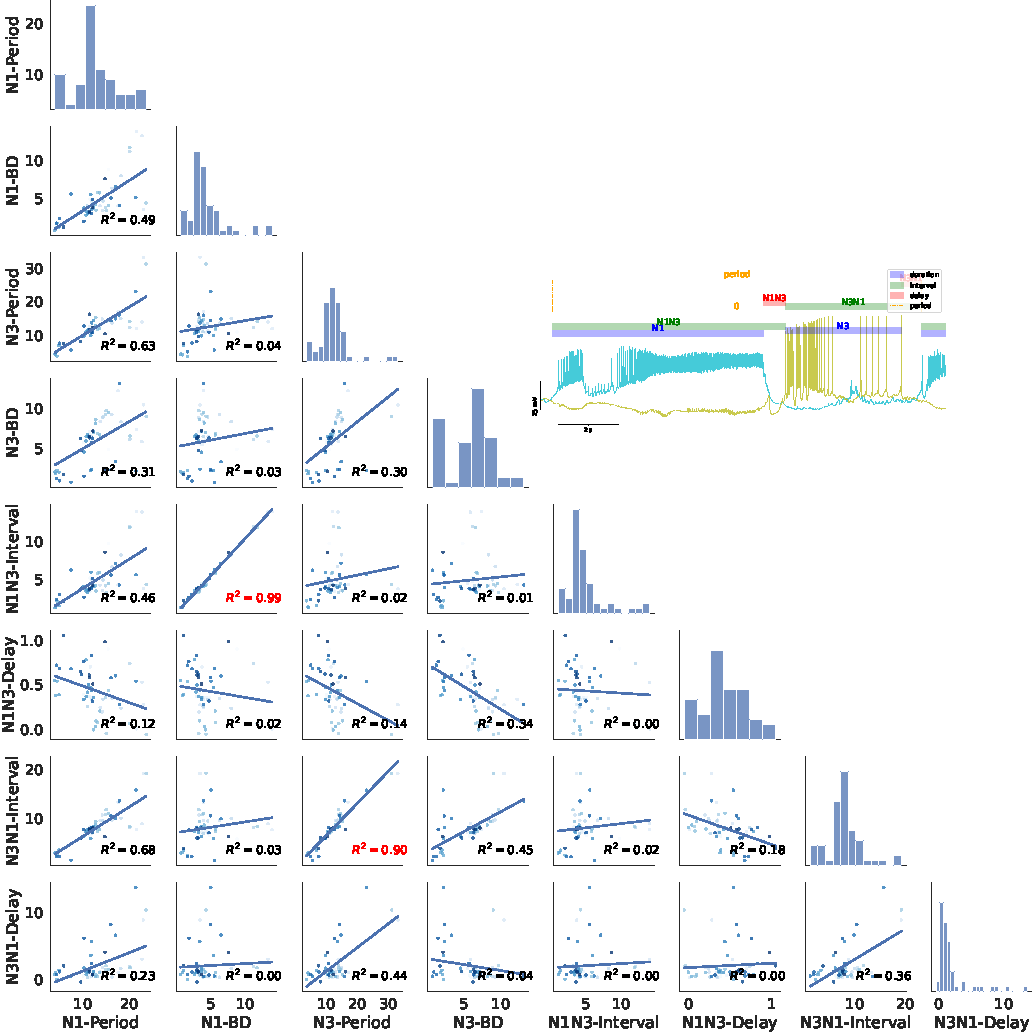
\includegraphics[width=0.48\textwidth]{./img/invariants/data/SUSSEX/prep3/images/2phases/panel_with_pairplot.pdf}
	\caption{}
	\label{fig:spontaneous pairplot comparison}
\end{figure}


\clearpage
\newpage
\subsection{Invariants in SO driven activity}
As we saw before, SO role in the feeding CPG is modulatory, which means, that modifies the rhythm once it is activated. In the model analysis, in section \ref{subsec:so driven} we showed that when the variability was induced modifying SO, the variability was distributed between the time intervals corresponding to N1 phase and N3 variability, and consequently increasing the R-squared values for the relation of both with the period. Therefore, in the living recordings we can expect that the variability cycle-by-cycle is distributed during the modulation of SO, which is connected to N1M and N3t (see Fig. \ref{fig:feeding distribution}). 

In this subsection we will see an example from a spontaneous activity that for two lapses of activity the SO is modulating, this is detected by the inhibition of B4 and activation of B3, in Fig. \ref{fig:SO-spontaneous-driven} this process is represented in the original data. In that figure it can also be seen how during the SO modulation, the rhythm is "stabilized" with less variability in the intervals duration. The characterization of the variability of the time intervals and their relation to the cycle period for this trace is depicted in Figs \ref{fig:so spontaneous invariants 1},\ref{fig:no so spontaneous invariants} and \ref{fig:so spontaneous invariants 2}, when SO is modulating, when it ceases its modulation and when it then restarts it, respectively. 


 \begin{figure}[htbp]
 	\centering
 	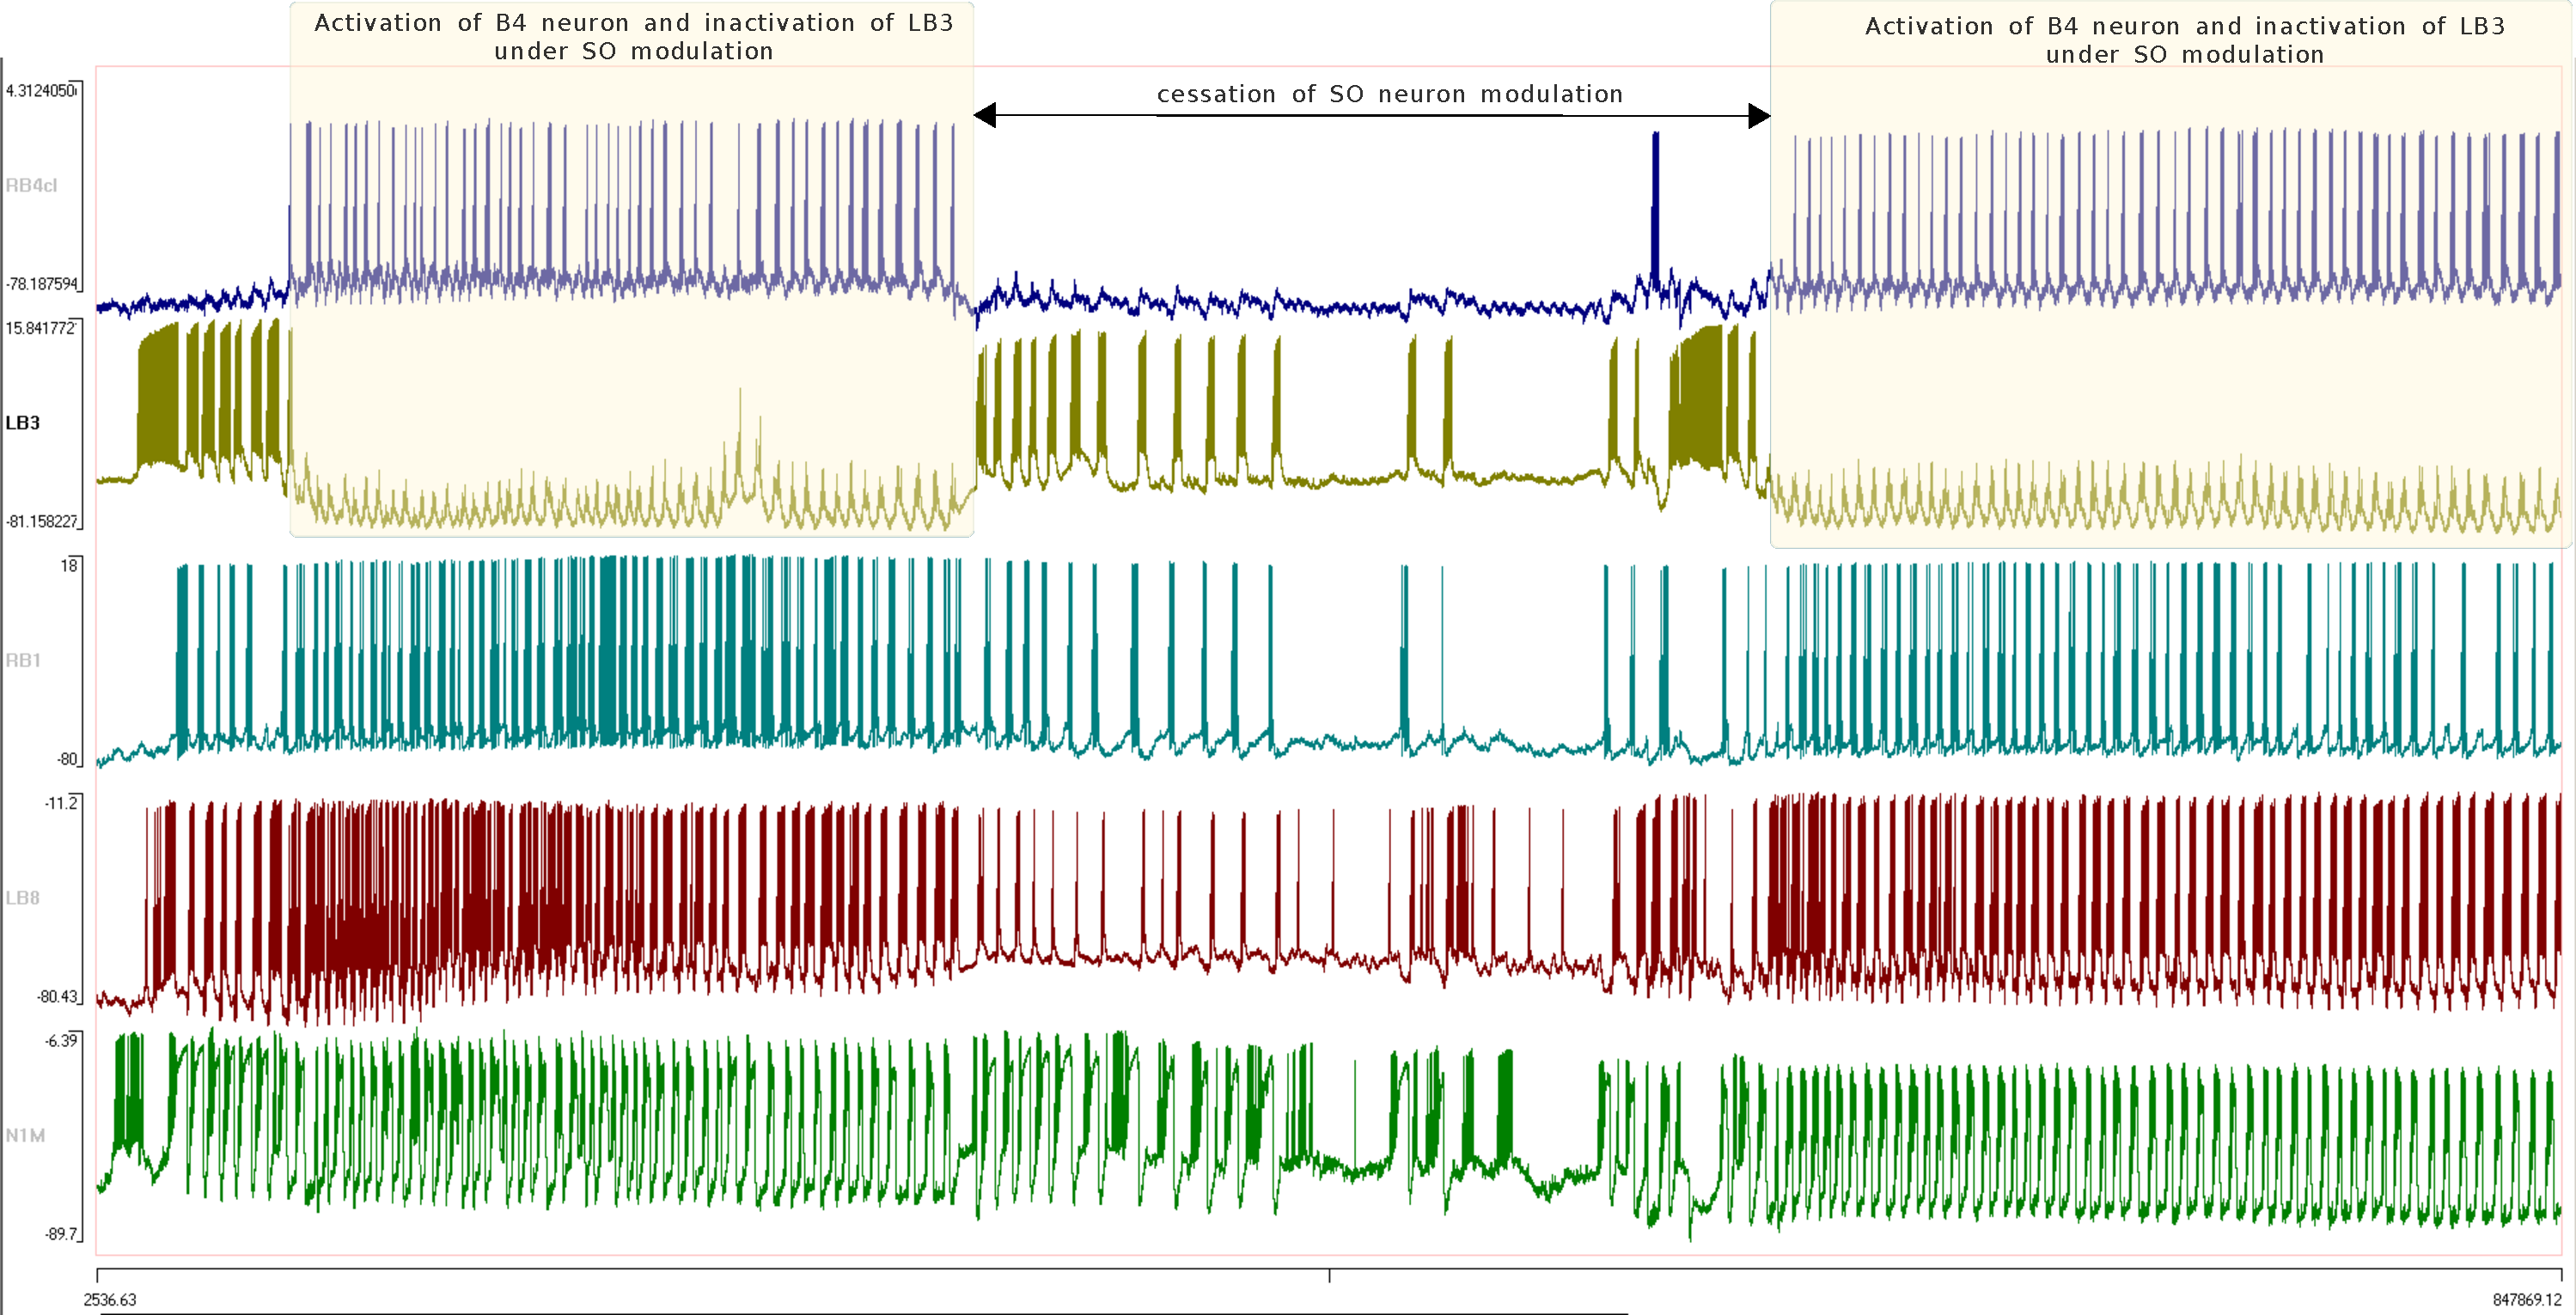
\includegraphics[width=\textwidth]{./img/invariants/SO-spontaneuous-driven.pdf}
 	\caption{Representation of the spontaneous recording with lapses of SO modulation. The parts of the recording with yellow background the activity was modulated by SO. From top to bottom, intracellular recording of a neuron from the B4 cluster, B3 motoneuron, B1 motoneuron, B8 motoneuron, N1M interneuron}
 	\label{fig:SO-spontaneous-driven}
 \end{figure}

While the rhythm is driven in SO we see how the variability for N1-BD and N3-BD increases, represented in the boxplots of Figs. \ref{fig:so spontaneous invariants 1} and \ref{fig:so spontaneous invariants 2}, and also in panel C. In the correlation of the intervals with the period, although R-square value is not significantly high, N1-BD and N3-BD have around 0.7 and 0.3 in both cases, pointing to this redistribution of the variability, since this is shifted in the period of time while SO stops its modulation. In Fig. \ref{fig:no so spontaneous invariants} the R-square value of N1-BD is in the order of 0.9, while the N3-BD not only low but close to 0 Although this example had only a few cycles, this suggest that the variability in that lapse of time is all carried in the N1 phase.  In the rest of the time-intervals in the cycle, this is extrapolated, being N3N1 interval the one with the largest variability and R-squared, since it contains N1-BD. Also, when activity ceases the N3N1 delay variability rises, which is notable compared to the rest of the experiments and the model, and might be caused by the burst shape and how the intervals where defined (see Fig. \ref{fig:no so spontaneous invariants}, first panel). This result, also matches the experimental work by \cite{elliott_temporal_1991}, that showed this distribution between N1-BD and N3-BD. In that work the SO modulation was induced by stimulating SO neuron, in Fig. \ref{fig:so induced driven invariants}

%Acabar comparación con el otro. 
 
\begin{figure}[htbp]
	\centering
	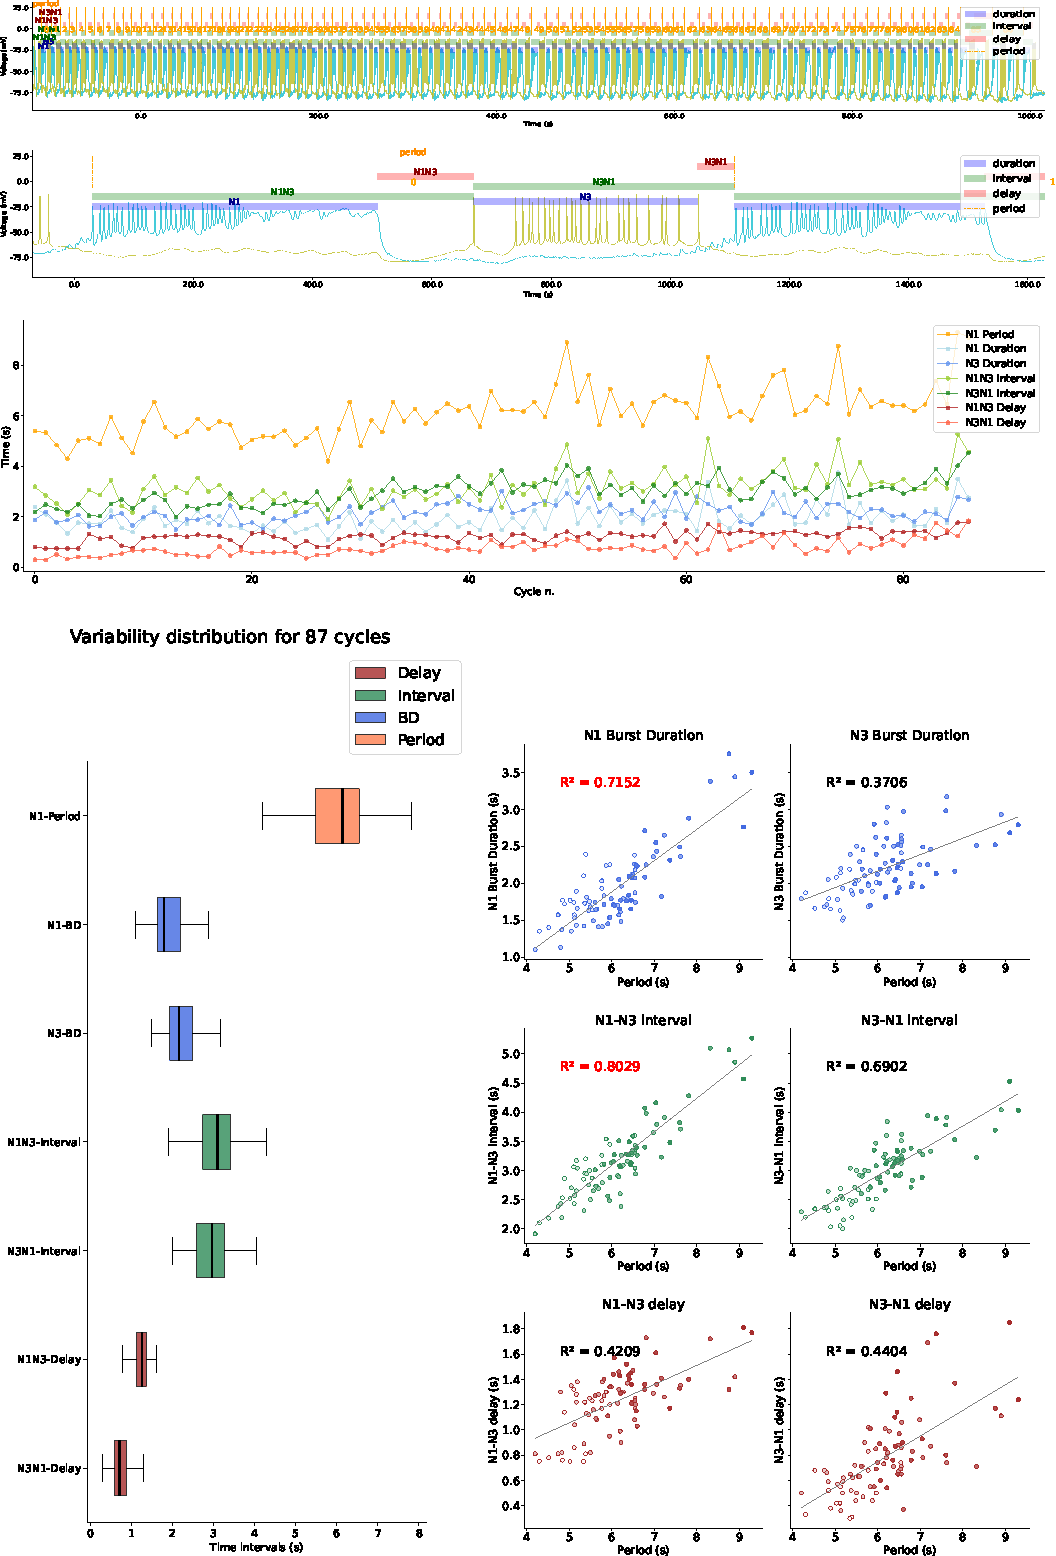
\includegraphics[width=0.95\textwidth]{./img/invariants/data/SUSSEX/prep4_so_driven_2/images/panel_with_intervals.pdf}
	\caption{\textbf{Spontaneous SO neuron driven}: Panel of intervals distribution and dynamical invariants for the two phases in the CPG for spontaneous activity driven by SO neuron.}
	\label{fig:so spontaneous invariants 2}
\end{figure}

%\begin{figure}[htbp]
%	\centering
%	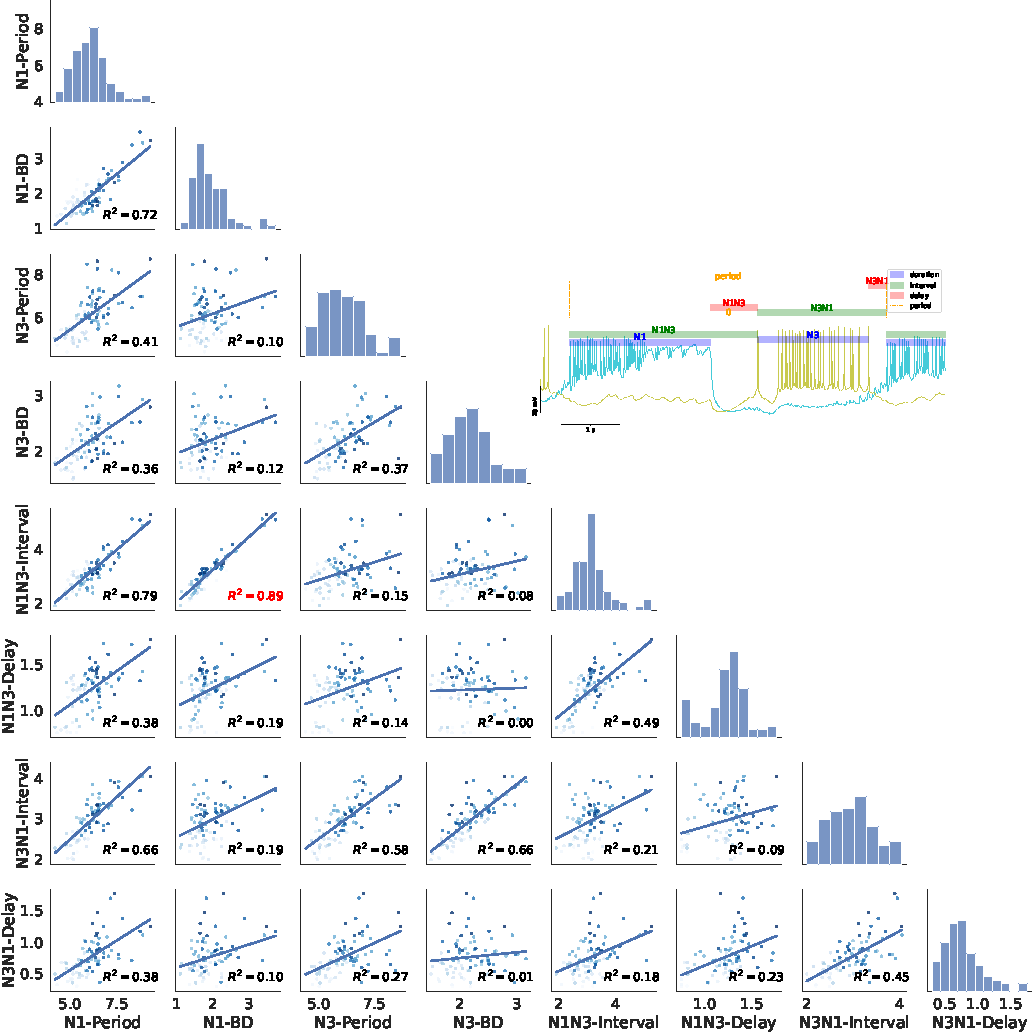
\includegraphics[width=0.9\textwidth]{./img/invariants/data/SUSSEX/prep4_so_driven_2/images/panel_with_pairplot.pdf}
%	\caption{\textbf{Spontaneous SO neuron driven}: Panel of intervals distribution and dynamical invariants for the two phases in the CPG for spontaneous activity driven by SO neuron.}
%	\label{fig:so spontaneous invariants pairplot 2}
%\end{figure}
% 	


\begin{figure}[htbp]
	\centering
	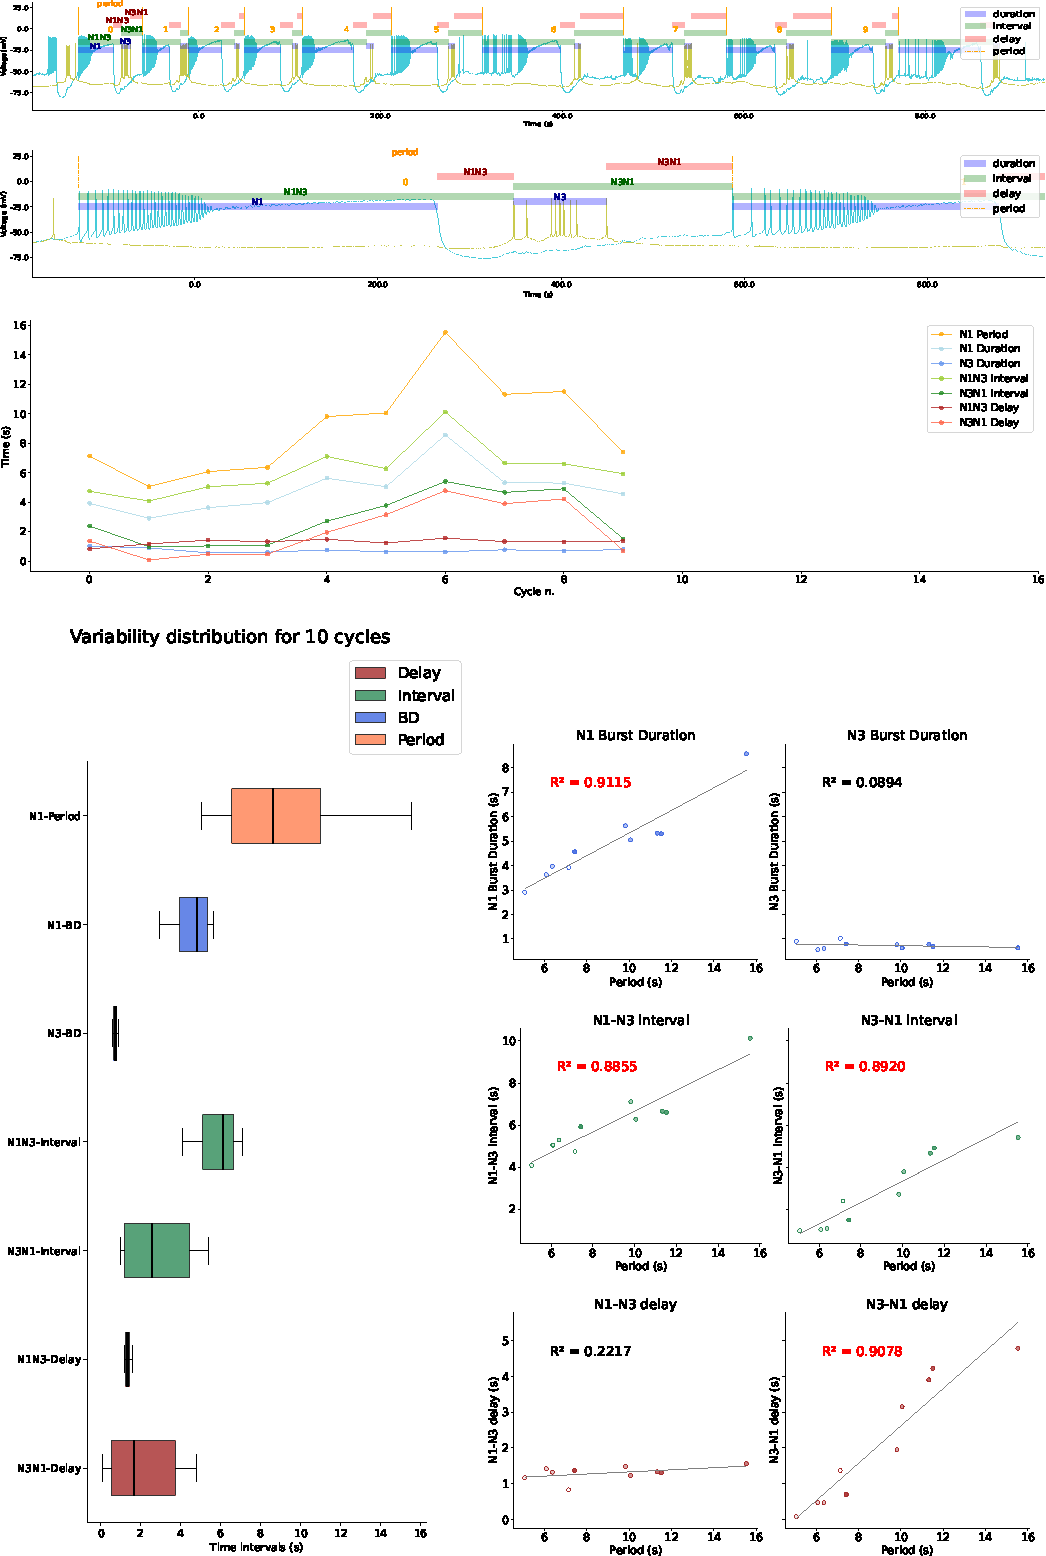
\includegraphics[width=0.95\textwidth]{./img/invariants/data/SUSSEX/prep4_so_no_driven/images/panel_with_intervals.pdf}
	\caption{\textbf{Spontaneous activity when SO-driven ceases}: Panel of intervals distribution and dynamical invariants for the three phases in the CPG for spontaneous activity.}
	\label{fig:no so spontaneous invariants}
\end{figure}
 	 
 
%\begin{figure}[htbp]
%	\centering
%	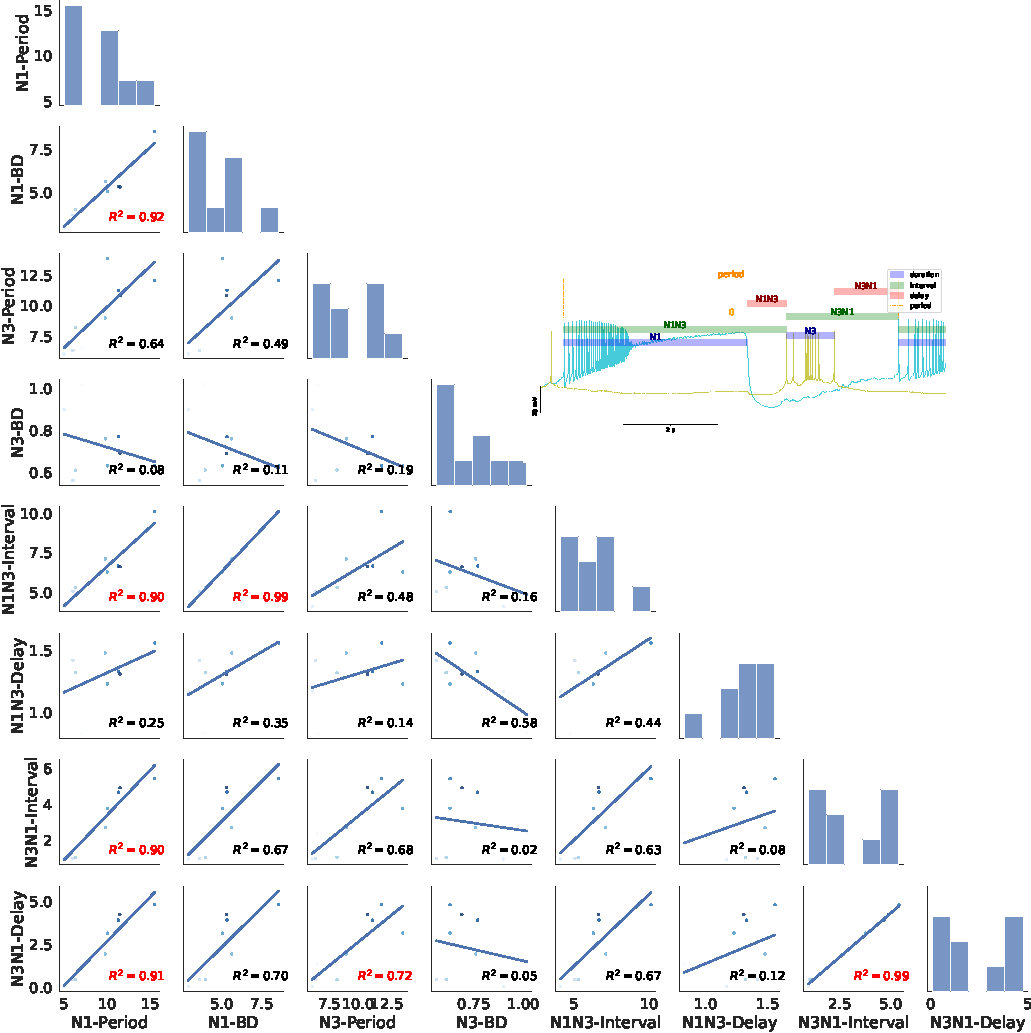
\includegraphics[width=0.9\textwidth]{./img/invariants/data/SUSSEX/prep4_so_no_driven/images/panel_with_pairplot.pdf}
%	\caption{\textbf{Spontaneous activity when SO-driven ceases}: Panel of intervals distribution and dynamical invariants for the three phases in the CPG for spontaneous activity.}
%	\label{fig:no so spontaneous invariants pairplot}
%\end{figure}


\begin{figure}[htbp]
	\centering
	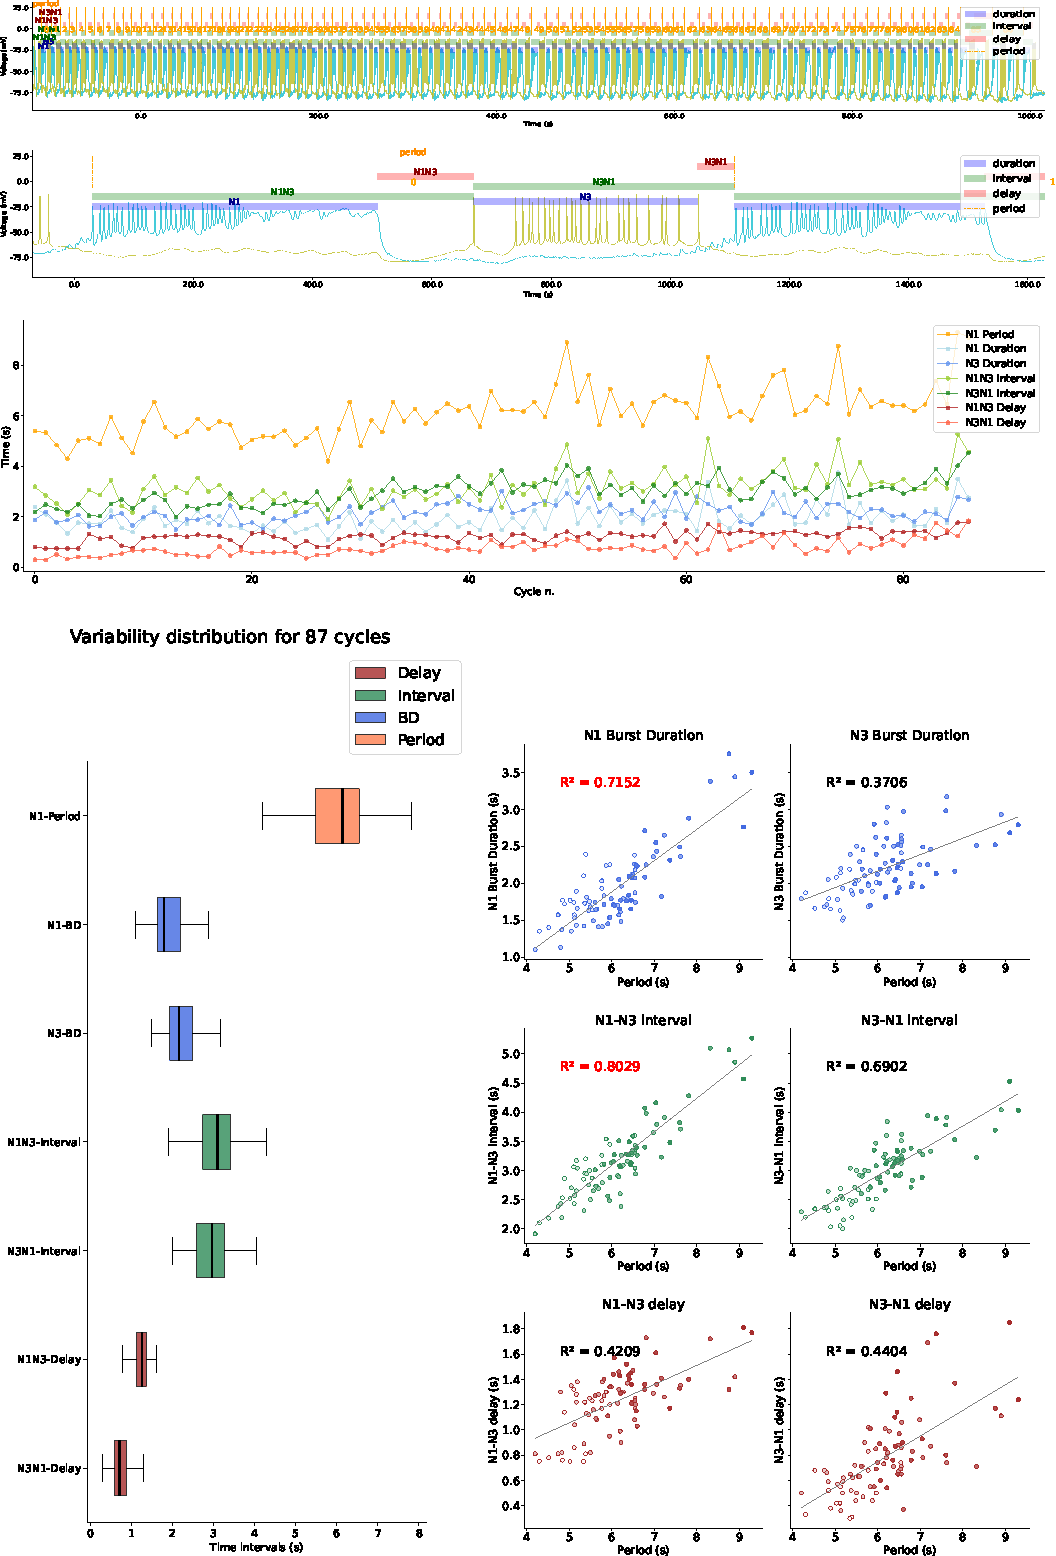
\includegraphics[width=0.95\textwidth]{./img/invariants/data/SUSSEX/prep4_so_driven_2/images/panel_with_intervals.pdf}
	\caption{\textbf{Spontaneous SO neuron modulation restarts}: Panel of intervals distribution and dynamical invariants for the two phases in the CPG for spontaneous activity driven by SO neuron.}
	\label{fig:so spontaneous invariants 1}
\end{figure}

%\begin{figure}[htbp]
%	\centering
%	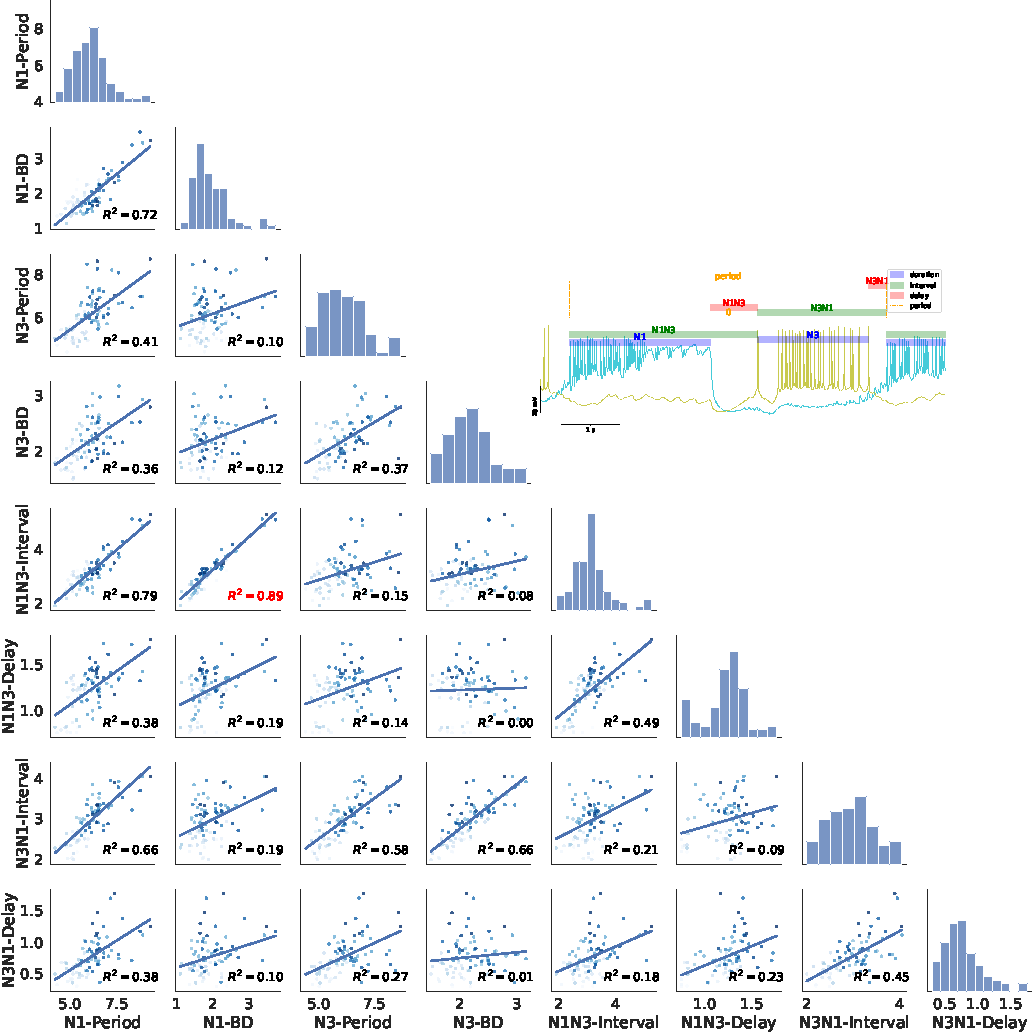
\includegraphics[width=0.9\textwidth]{./img/invariants/data/SUSSEX/prep4_so_driven_2/images/panel_with_pairplot.pdf}
%	\caption{\textbf{Spontaneous SO neuron driven}: Panel of intervals distribution and dynamical invariants for the two phases in the CPG for spontaneous activity driven by SO neuron.}
%%	\label{fig:so spontaneous invariants pairplot 2}
%\end{figure}


\begin{figure}[htbp]
	\centering
	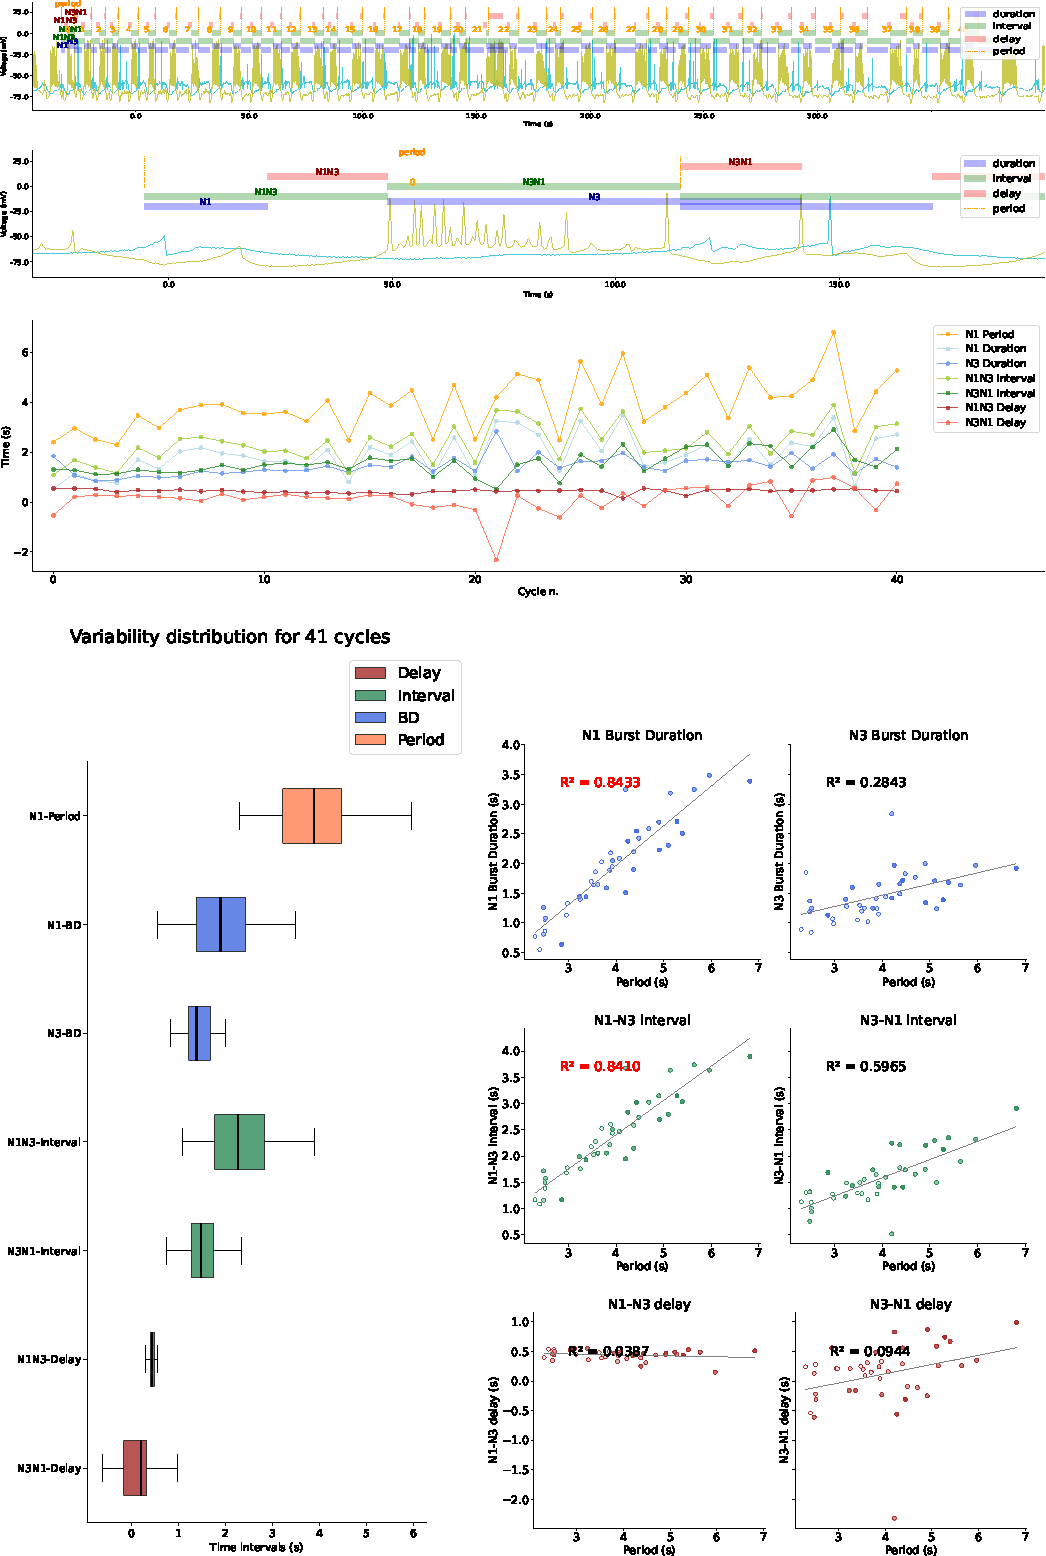
\includegraphics[width=0.95\textwidth]{./img/invariants/data/SUSSEX/SO_driven/images/panel_with_intervals.pdf}
	\caption{\textbf{Spontaneous SO neuron driven}: Panel of intervals distribution and dynamical invariants for the two phases in the CPG for activity driven by SO neuron induced by its electrical stimulation.}
	\label{fig:so induced invariants}
\end{figure}

 
\begin{figure}[htbp]
	\centering
	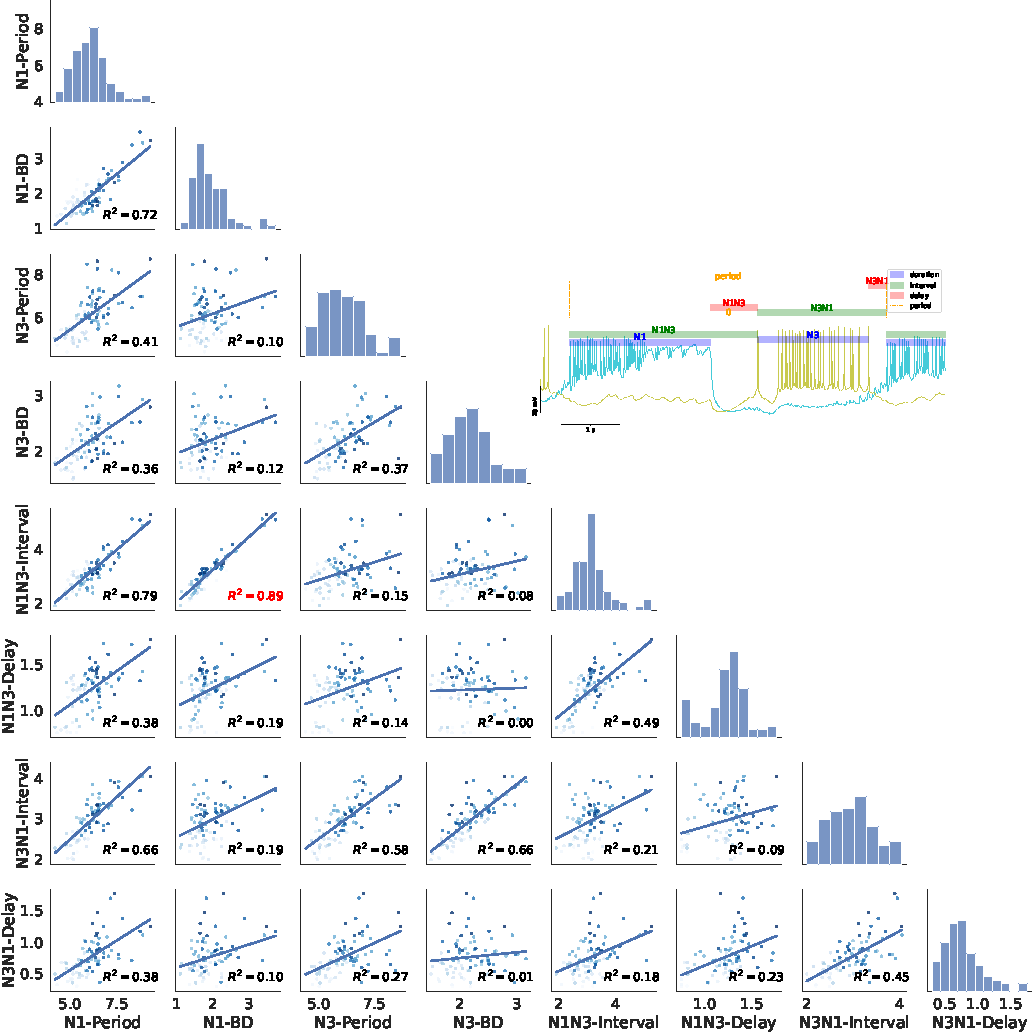
\includegraphics[width=0.48\textwidth]{./img/invariants/data/SUSSEX/prep4_so_driven_2/images/panel_with_pairplot.pdf}
	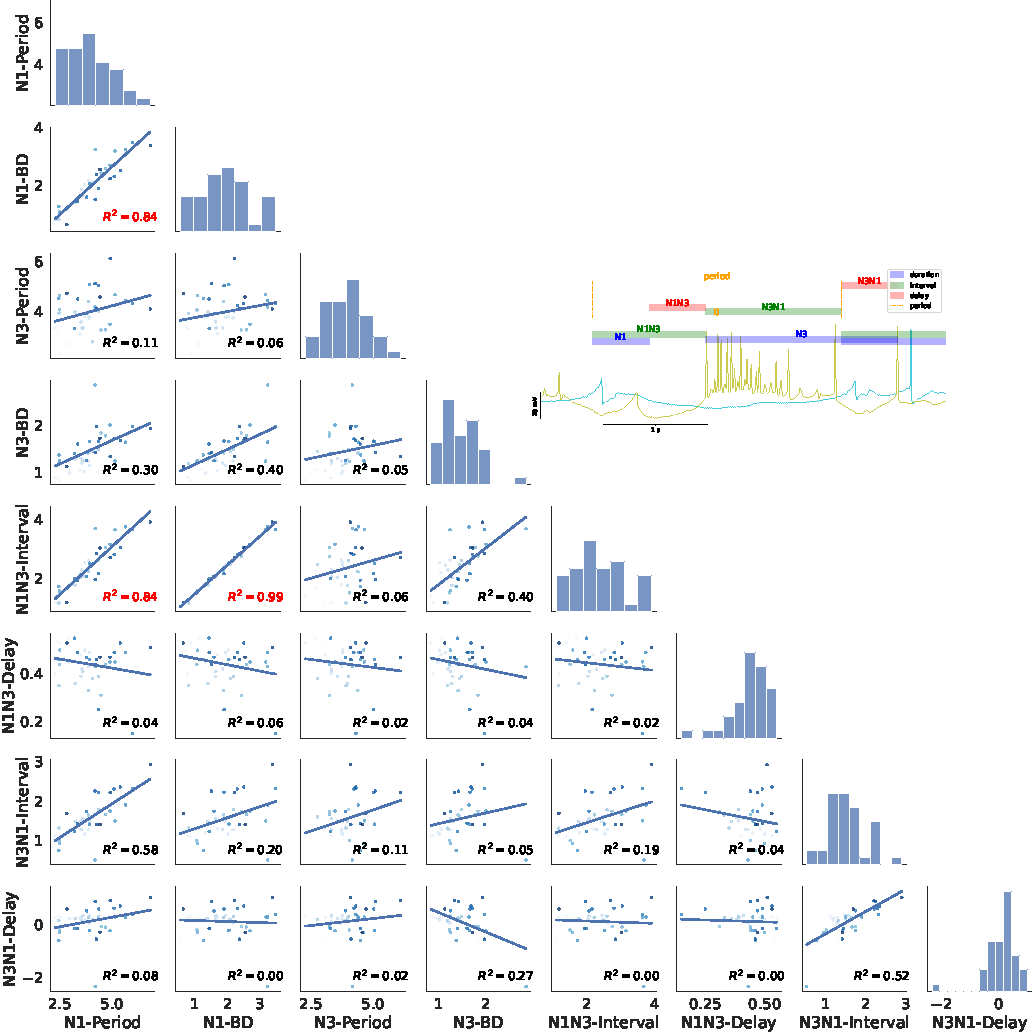
\includegraphics[width=0.48\textwidth]{./img/invariants/data/SUSSEX/SO_driven/images/panel_with_pairplot.pdf}
	\caption{\textbf{Left: Spontaneous SO rhythm modulation.} Panel of the pairplot for all possible combinations between the time intervals for two phases in the CPG in the spontaneous activity driven by SO neuron. \textbf{Right: Induced SO rhythm modulation.} Panel of the pairplot for all possible combinations between the time intervals for two phases in the CPG under SO modulatory neuron stimulation.}
	\label{fig:so pairplot comparison}
\end{figure}

\subsection{Invariants in MLN stimulation driven activity}
The snail's lips are connected to the cerebral ganglia by the MLN (median lip nerves). It is possible to stimulate CPG activity by its stimulation, simulating the initiation of the rhythm in food presence \parencite{staras_electrophysiological_2019}. The data in this recording was stimulated by (4volt 1Hz stim).


\begin{figure}[htbp]
	\centering
	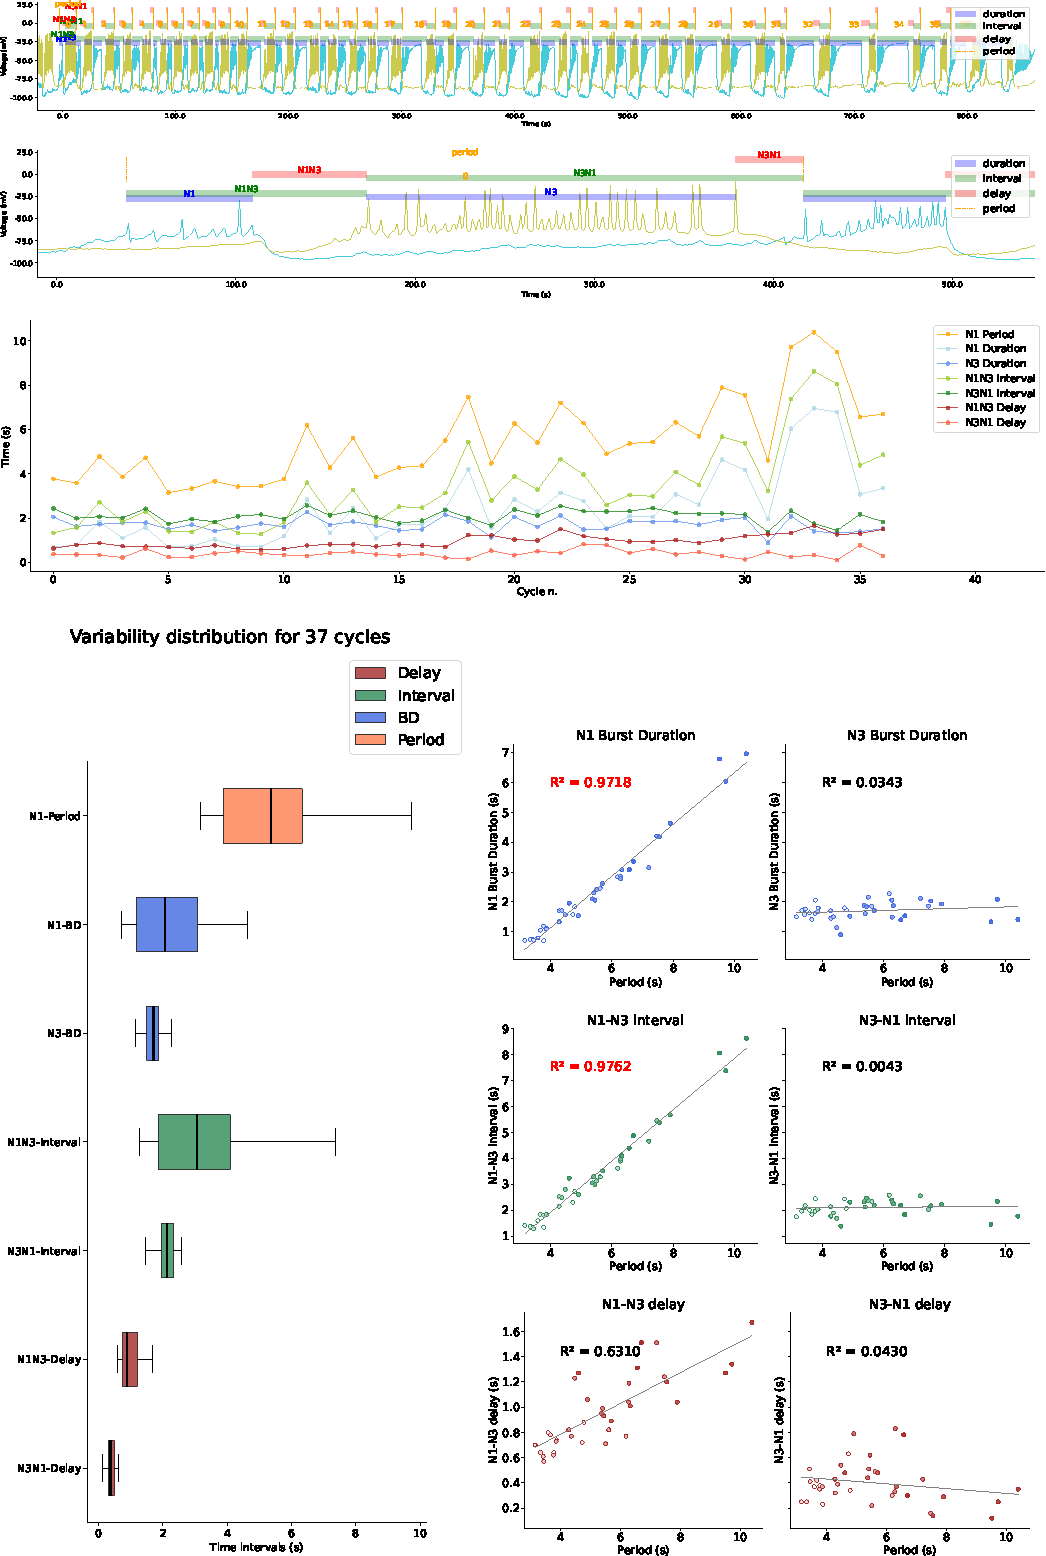
\includegraphics[width=0.9\textwidth]{./img/invariants/data/SUSSEX/MLN_driven/images/panel_with_intervals.pdf}
	\caption{\textbf{MLN stimulation}: Panel of intervals distribution and dynamical invariants for the three phases in the CPG under MLN Medium Lip Nerve (MLN) stimulation.}
	\label{fig:mln stimulation}
\end{figure}


\begin{figure}[htbp]
	\centering
	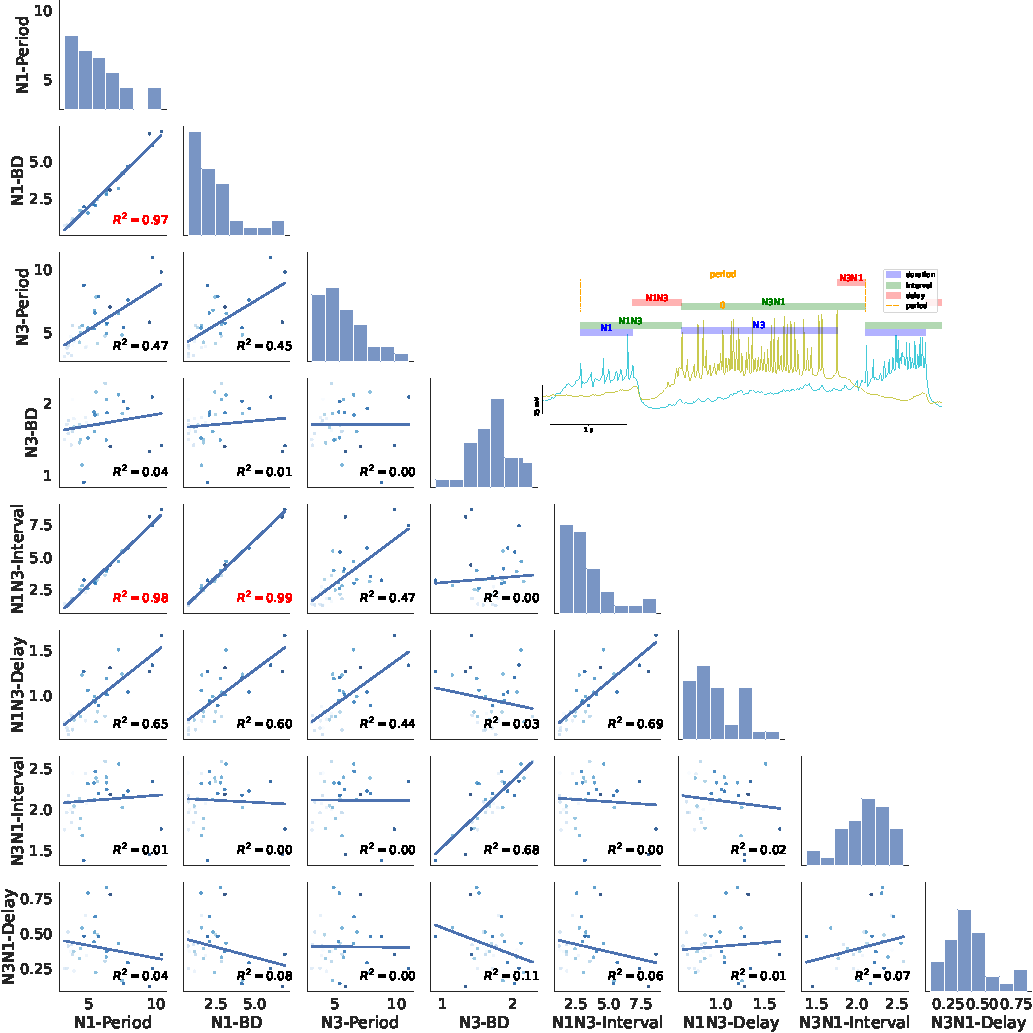
\includegraphics[width=0.9\textwidth]{./img/invariants/data/SUSSEX/MLN_driven/images/panel_with_pairplot.pdf}
	\caption{\textbf{MLN stimulation}:Pairplot of the invariants reset within cycles.}
	\label{fig:mln stimulation pairplot}
\end{figure}


\begin{figure}[htbp]
	\centering
	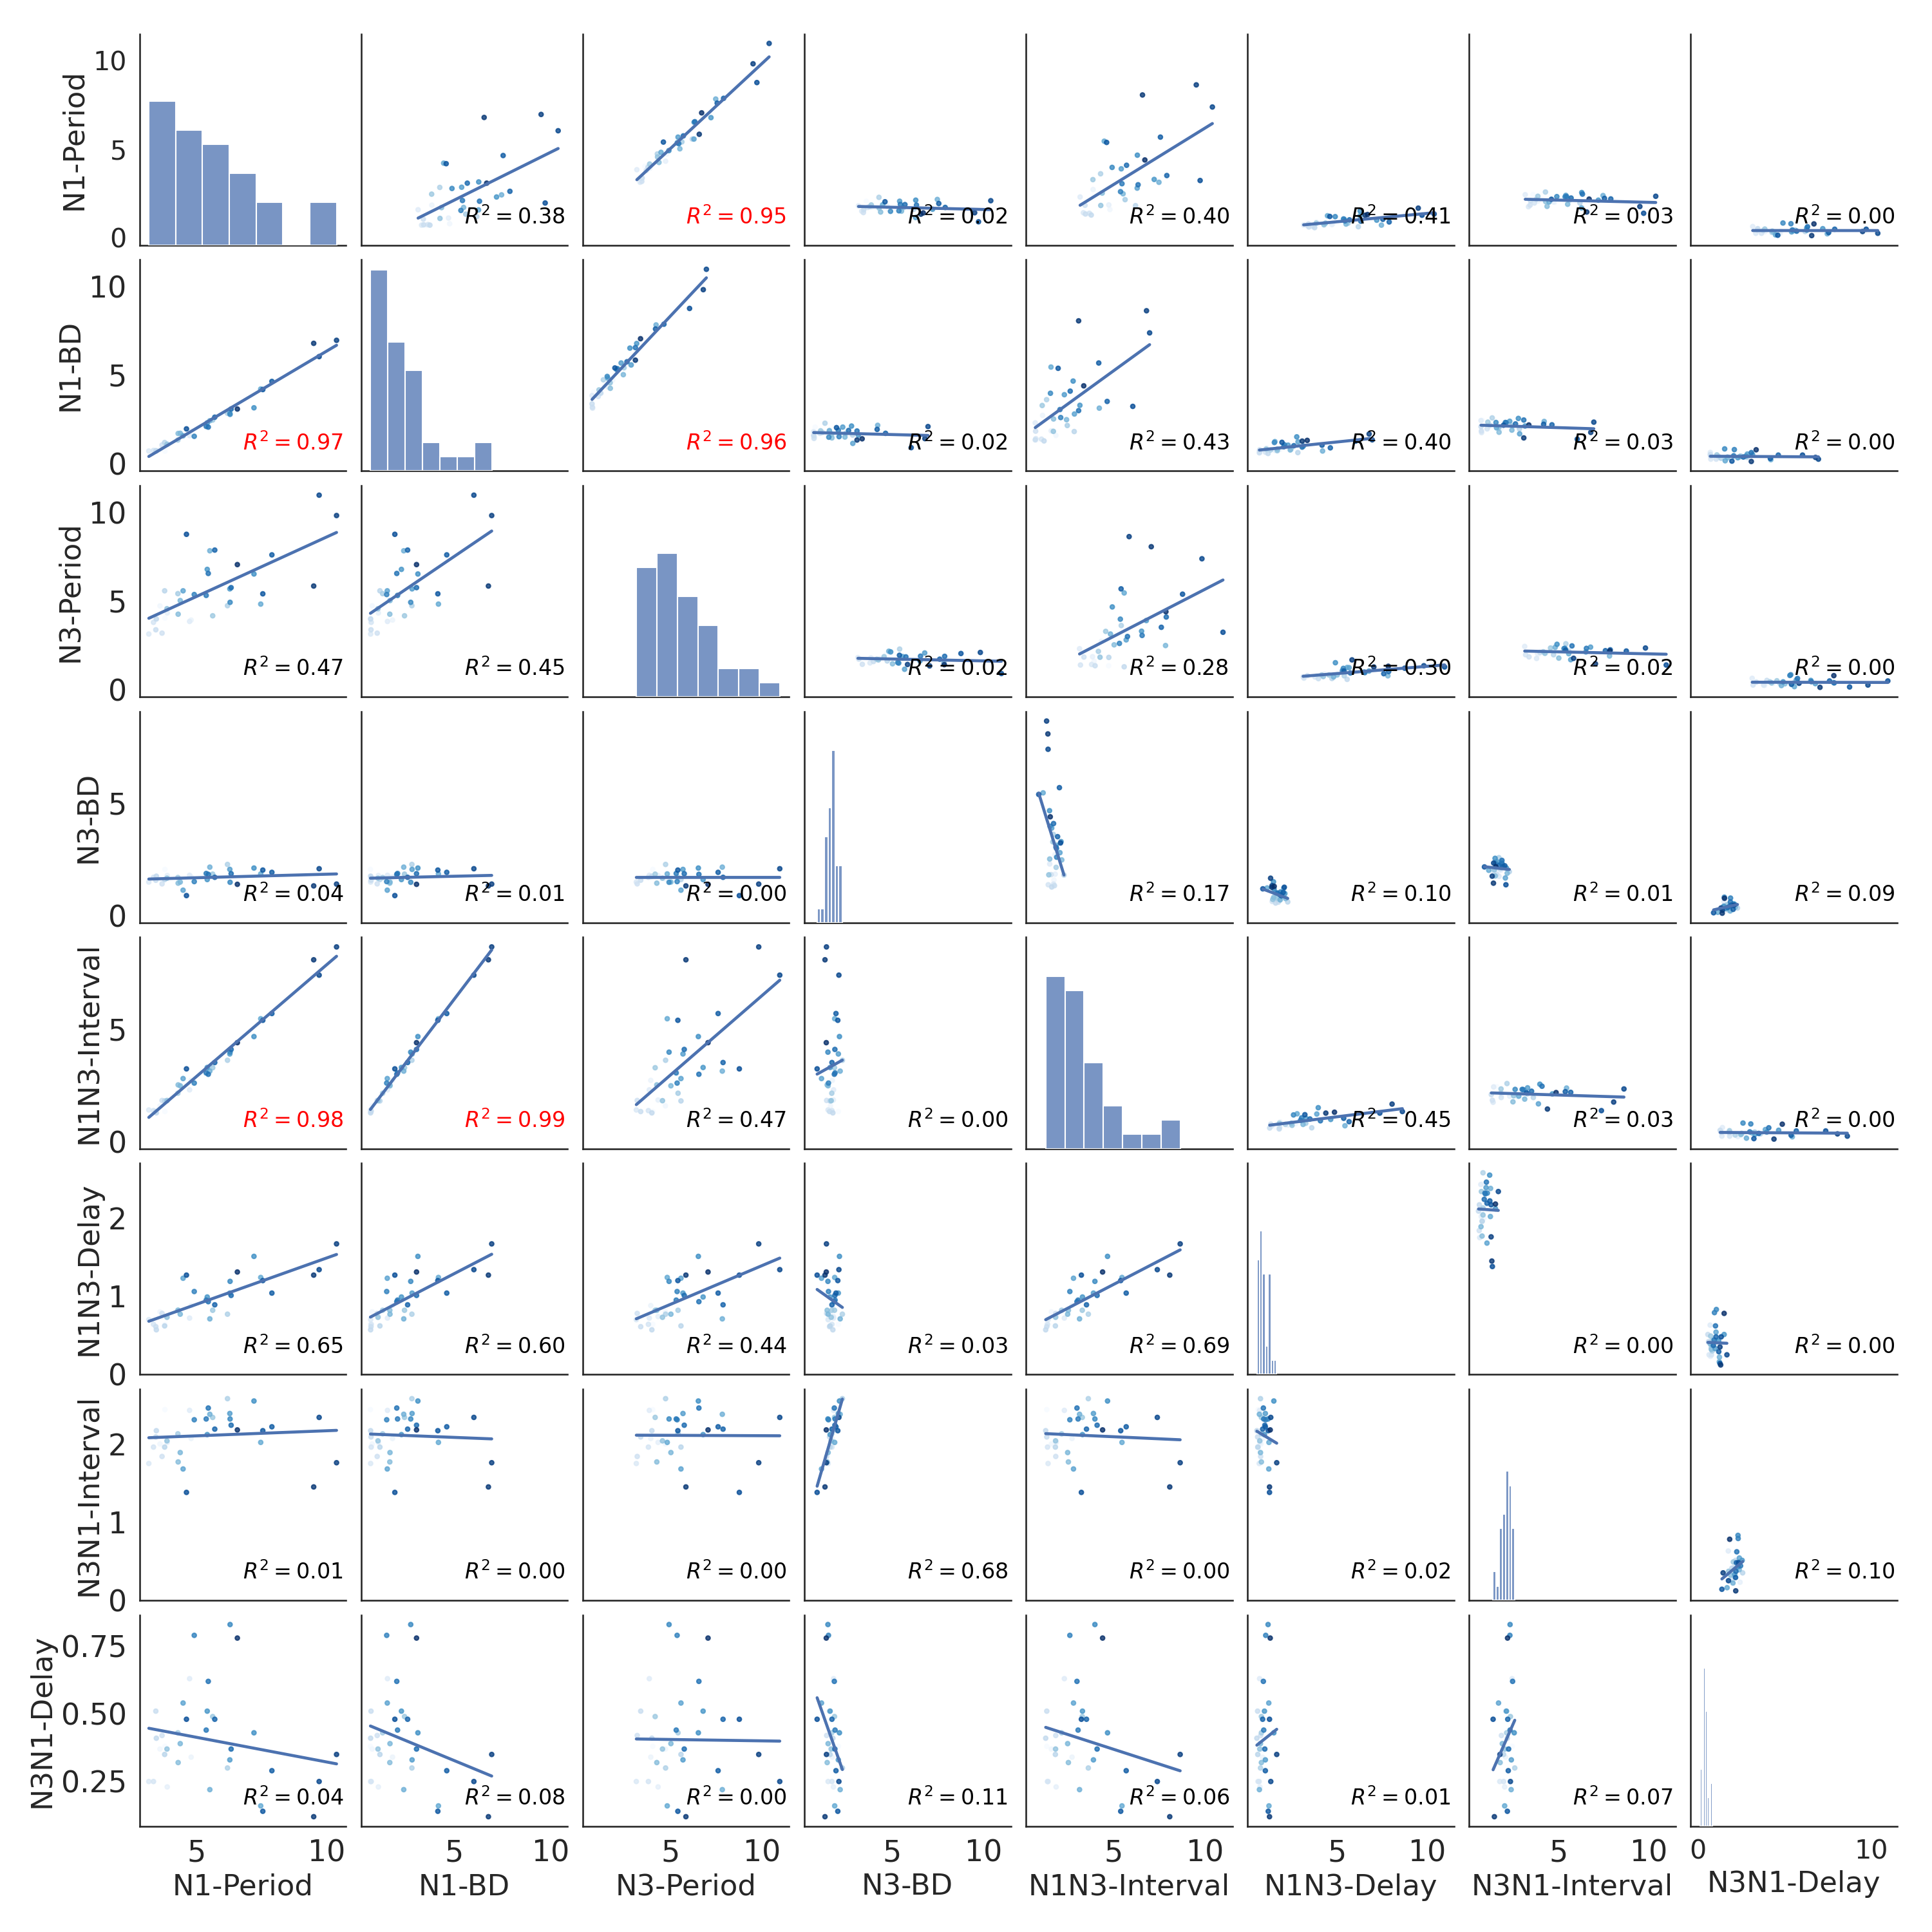
\includegraphics[width=0.9\textwidth]{./img/invariants/data/SUSSEX/MLN_driven/images/_output_pairplot_reset.png}
	\caption{\textbf{MLN stimulation}: Panel of intervals distribution and dynamical invariants for the three phases in the CPG under MLN Medium Lip Nerve (MLN) stimulation.}
	\label{fig:mln stimulation reset pairplot}
\end{figure}


\subsection{Invariants in cva1 stimulation driven activity}
CV1a neuron is part of a larger population of CBIs that is influeced by sucrose, which can drive the rhythmic activity in that group of neurons. CBIs are connected by mutual excitation to interneuron N1M, influencing the activation of the rhythm (see Fig. \ref{fig:feeding distribution}). 
%
%%and the complete map of their locations is shown in Figure 3A. https://static-content.springer.com/esm/art%3A10.1186%2F2042-1001-2-4/MediaObjects/13232_2011_20_MOESM3_ESM.jpeg
%Sucrose drives rhythmic activity in CBIs activating the feeding circuit by the conection
\paragraph{Example 1}

%\begin{figure}[htbp]
%	\centering
%	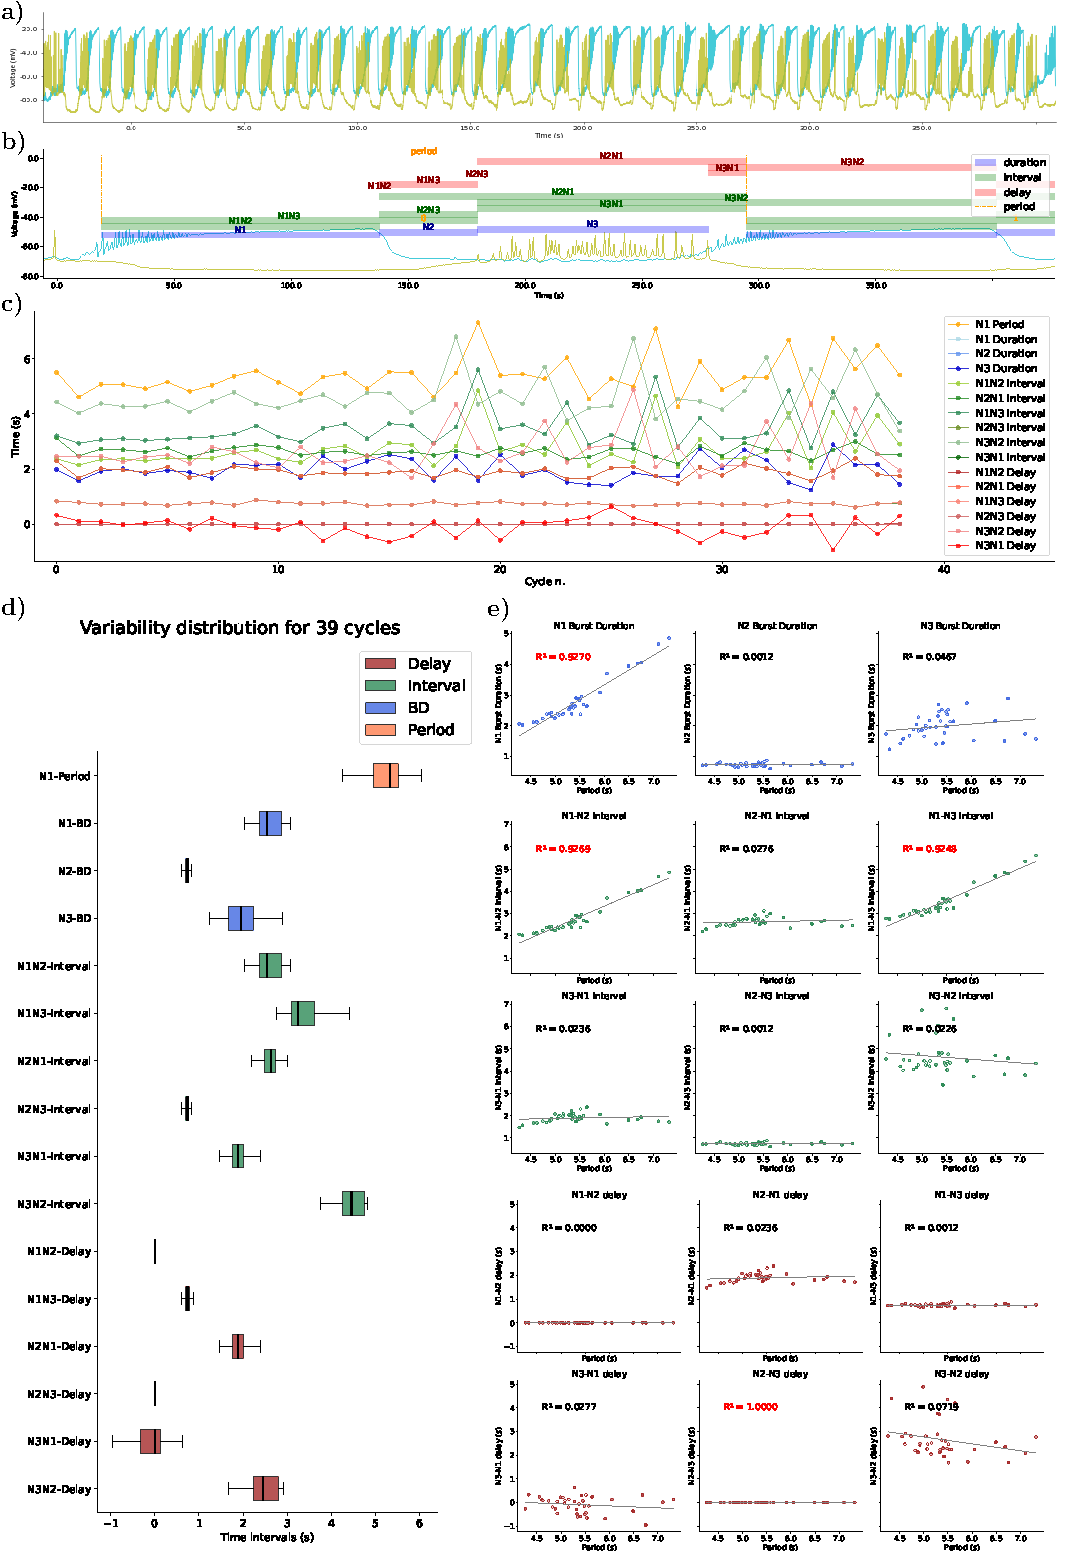
\includegraphics[width=0.9\textwidth]{./img/invariants/data/SUSSEX/CV1a_driven1/images/3phases/panel_with_intervals.pdf}
%	\caption{\textbf{CV1a driven case1}: Panel of intervals distribution and dynamical invariants for the three phases in the CPG under CV1a stimulation.}
%	\label{fig:cv1a 1 3phases}
%\end{figure}
%
%\begin{figure}[htbp]
%	\centering
%	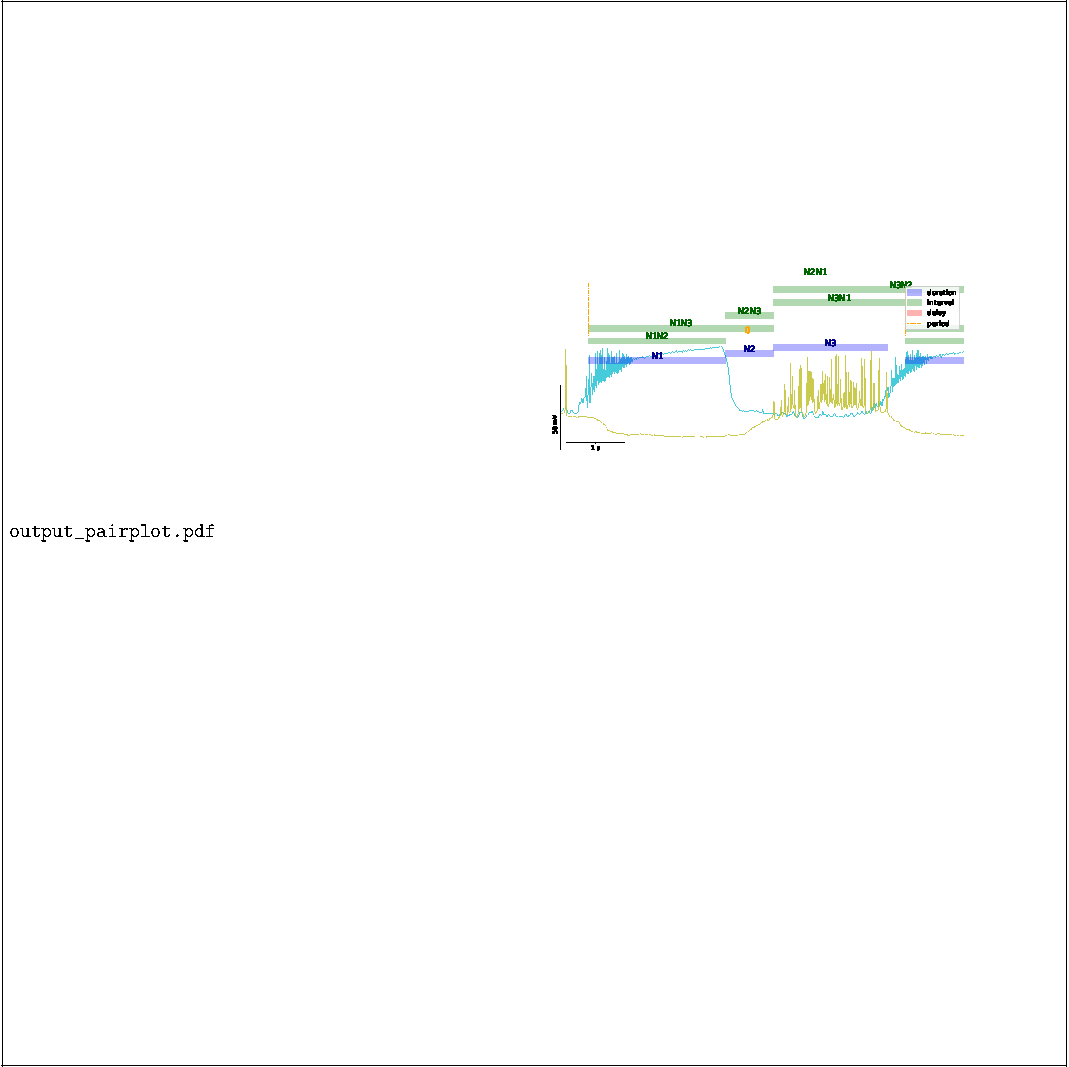
\includegraphics[width=0.9\textwidth]{./img/invariants/data/SUSSEX/CV1a_driven1/images/3phases/panel_with_pairplot.pdf}
%	\caption{\textbf{CV1a driven case1}: Panel of intervals distribution and dynamical invariants for the three phases in the CPG under CV1a stimulation.}
%	\label{fig:cv1a 1 3phases pairplot}
%\end{figure}

\begin{figure}[htbp]
	\centering
	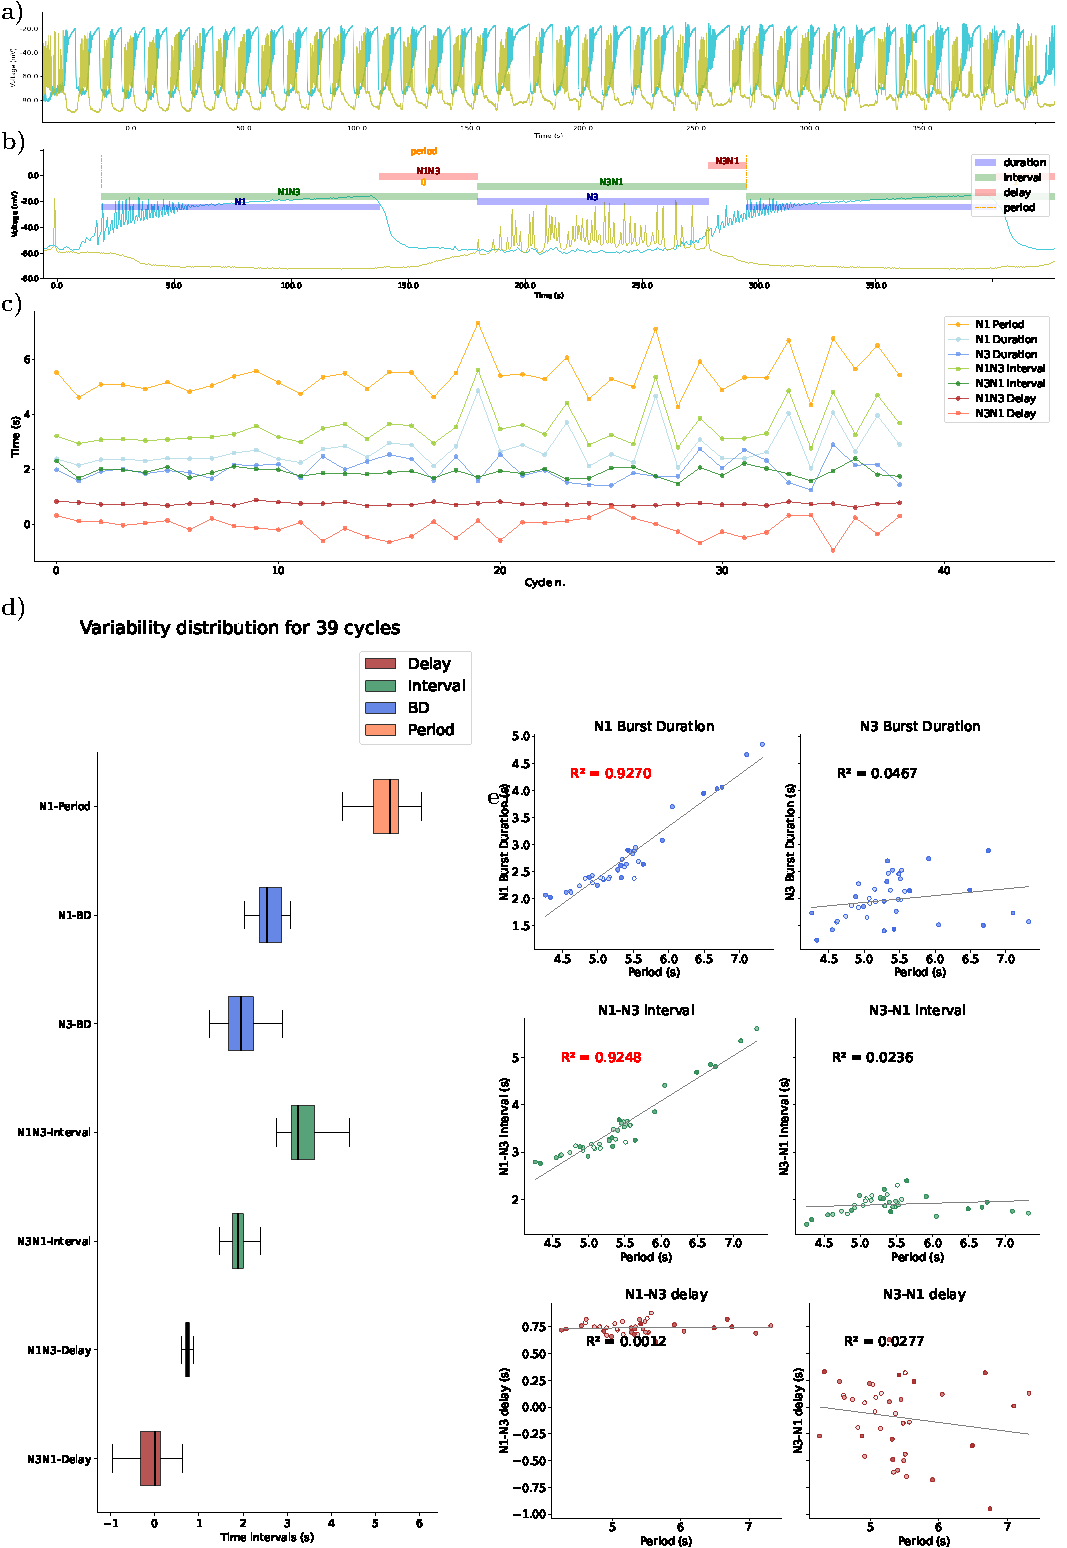
\includegraphics[width=0.9\textwidth]{./img/invariants/data/SUSSEX/CV1a_driven1/images/2phases/panel_with_intervals.pdf}
	\caption{\textbf{CV1a driven case1}:Panel of intervals distribution and dynamical invariants for the two phases in the CPG under CV1a stimulation.}
	\label{fig:cv1a 1 2phases}
\end{figure}

%
%\begin{figure}[htbp]
%	\centering
%	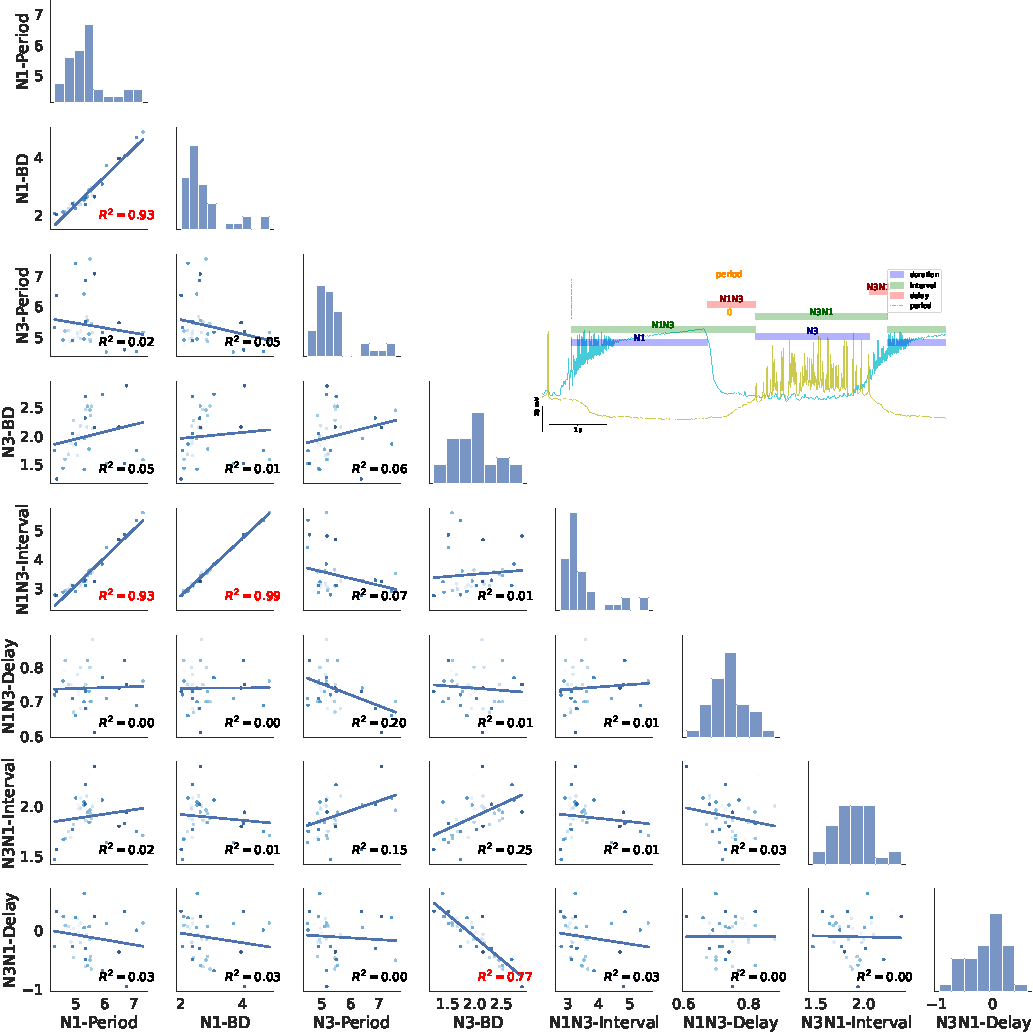
\includegraphics[width=0.9\textwidth]{./img/invariants/data/SUSSEX/CV1a_driven1/images/2phases/panel_with_pairplot.pdf}
%	\caption{\textbf{CV1a driven case1}:Panel of intervals distribution and dynamical invariants for the two phases in the CPG under CV1a stimulation.}
%	\label{fig:cv1a 1 2phases pairplot}
%\end{figure}



\paragraph{Example 2}


\begin{figure}[htbp]
	\centering
	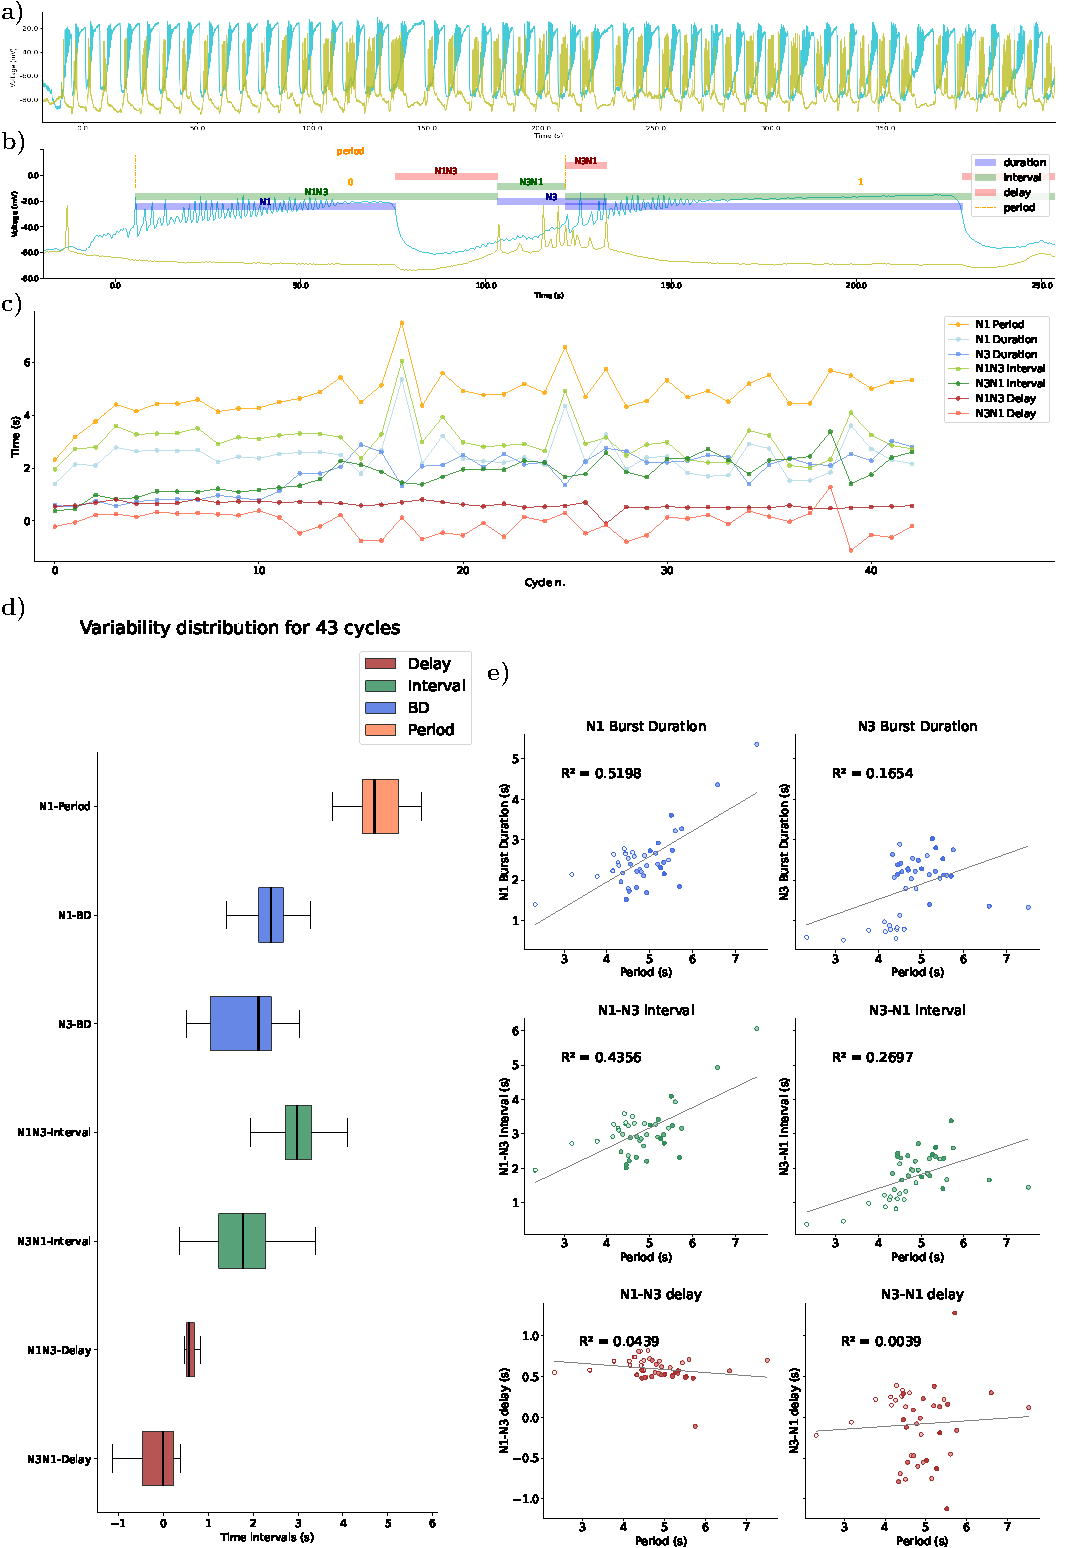
\includegraphics[width=0.9\textwidth]{./img/invariants/data/SUSSEX/CV1a_driven2/images/panel_with_intervals.pdf}
	
	\caption{\textbf{CV1a driven case2}: Panel of intervals distribution and dynamical invariants for the two phases in the CPG under CV1a stimulation.}
	\label{fig:cv1a 2 2phases}
\end{figure}

%
%\begin{figure}[htbp]
%	\centering
%	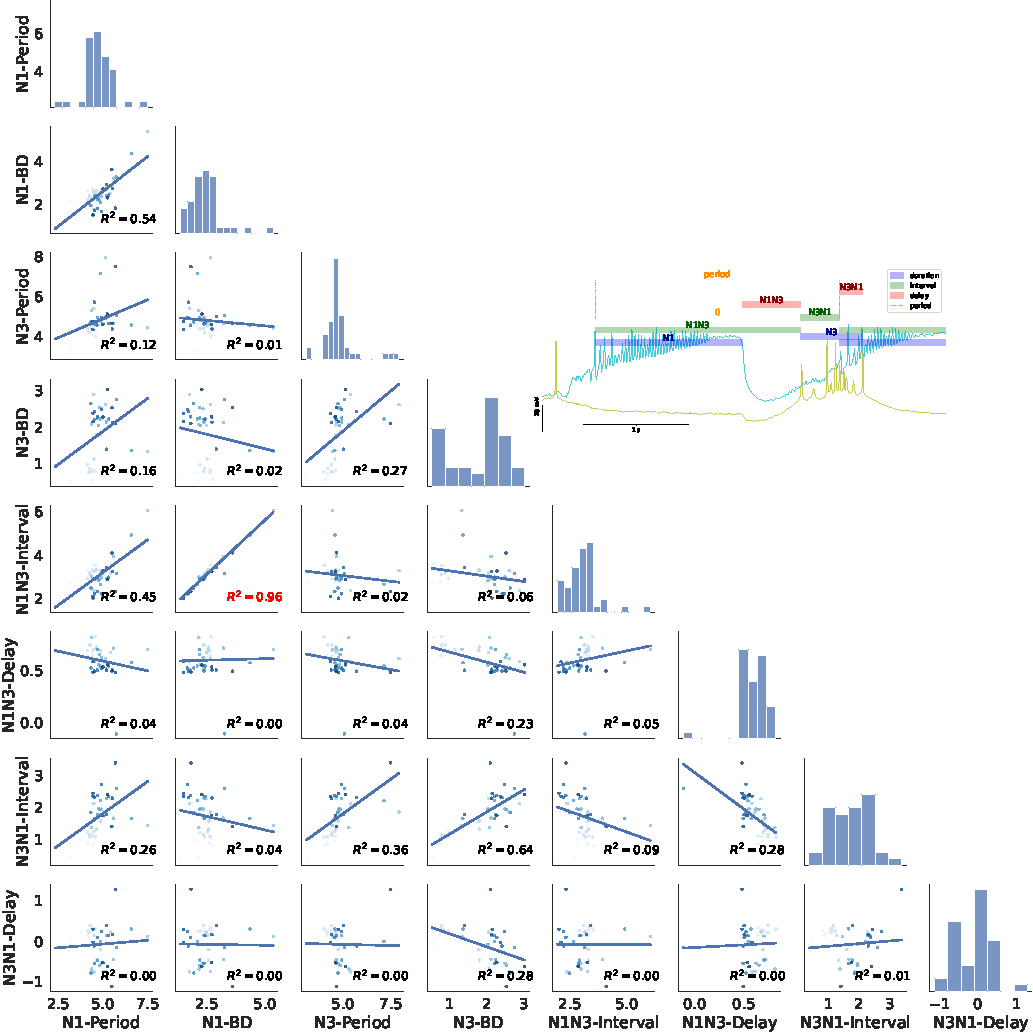
\includegraphics[width=0.9\textwidth]{./img/invariants/data/SUSSEX/CV1a_driven2/images/panel_with_pairplot.pdf}
%	
%	\caption{\textbf{CV1a driven case2}: Panel of intervals distribution and dynamical invariants for the two phases in the CPG under CV1a stimulation.}
%	\label{fig:cv1a 2 2phases pairplot}
%\end{figure}




\paragraph{Example 3}


\begin{figure}[htbp]
	\centering
	\includegraphics[width=0.9\textwidth]{./img/invariants/data/SUSSEX/CV1a_driven3/images/panel_with_intervals.pdf}
	\caption{\textbf{CV1a driven case3}: Panel of intervals distribution and dynamical invariants for the two phases in the CPG under CV1a stimulation.}
	\label{fig:cv1a 3 2phases}
\end{figure}



\paragraph{Example 4}

%\begin{figure}[htbp]
%	\centering
%	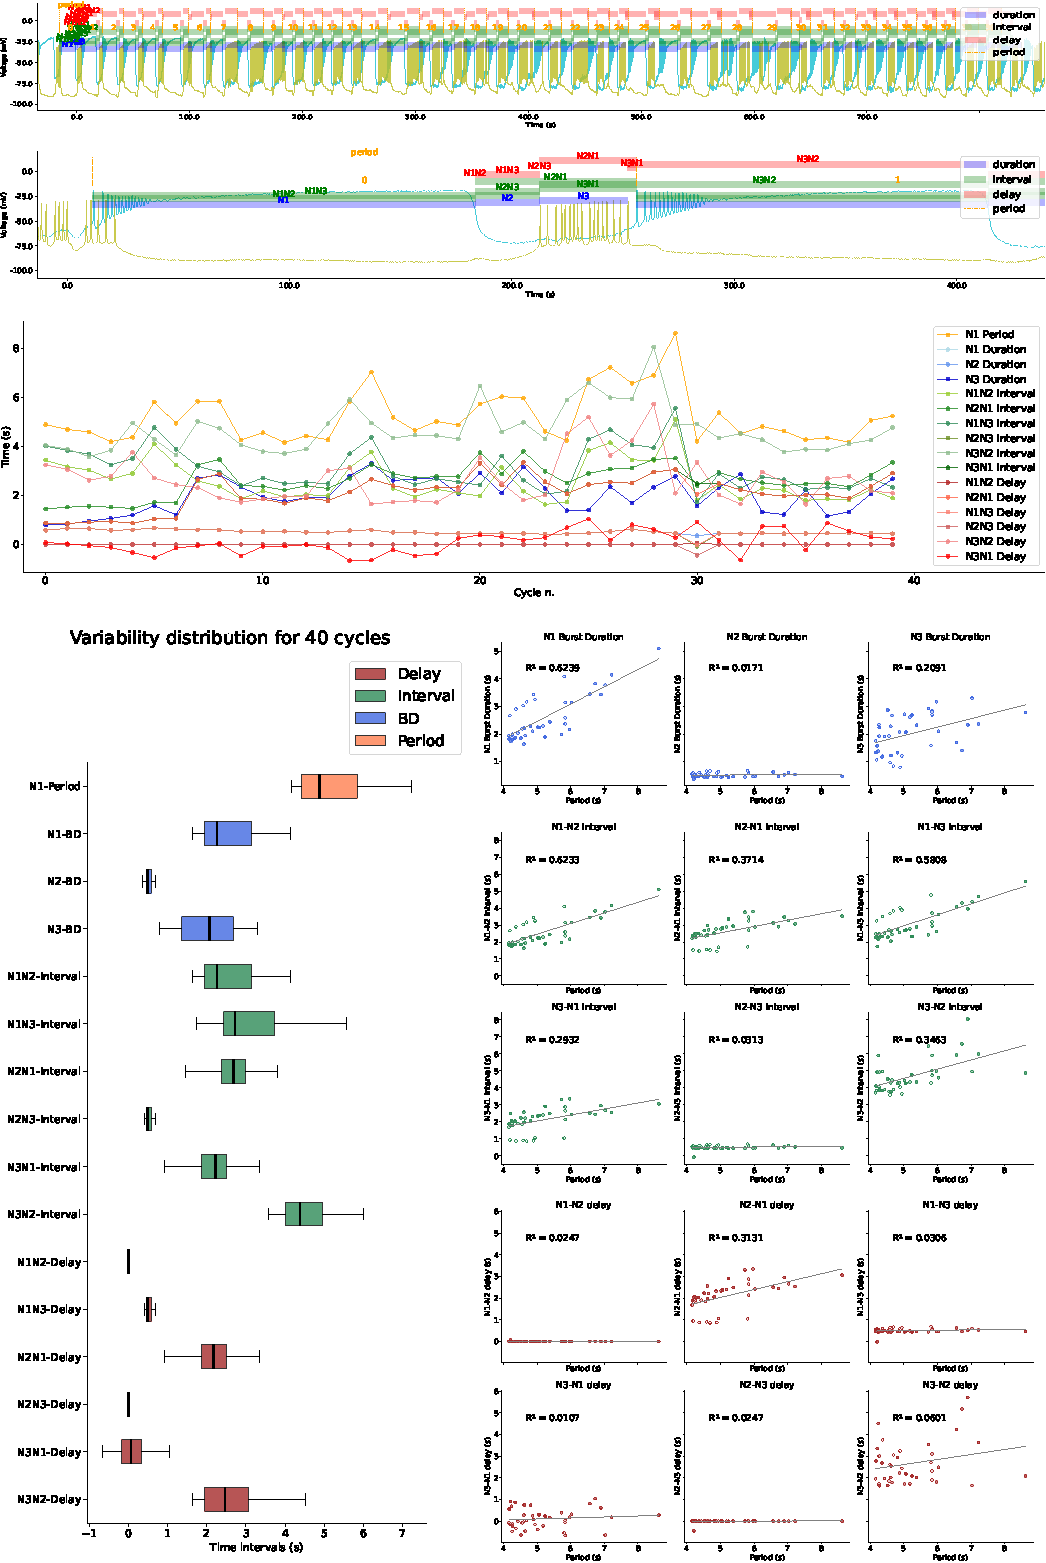
\includegraphics[width=0.9\textwidth]{./img/invariants/data/SUSSEX/CV1a_driven4/images/3phases/panel_with_intervals.pdf}
%	\caption{\textbf{CV1a driven case 4}: Panel of intervals distribution and dynamical invariants for the three phases in the CPG under CV1a stimulation.}
%	\label{fig:cv1a 4 3phases}
%\end{figure}
%
%\begin{figure}[htbp]
%	\centering
%	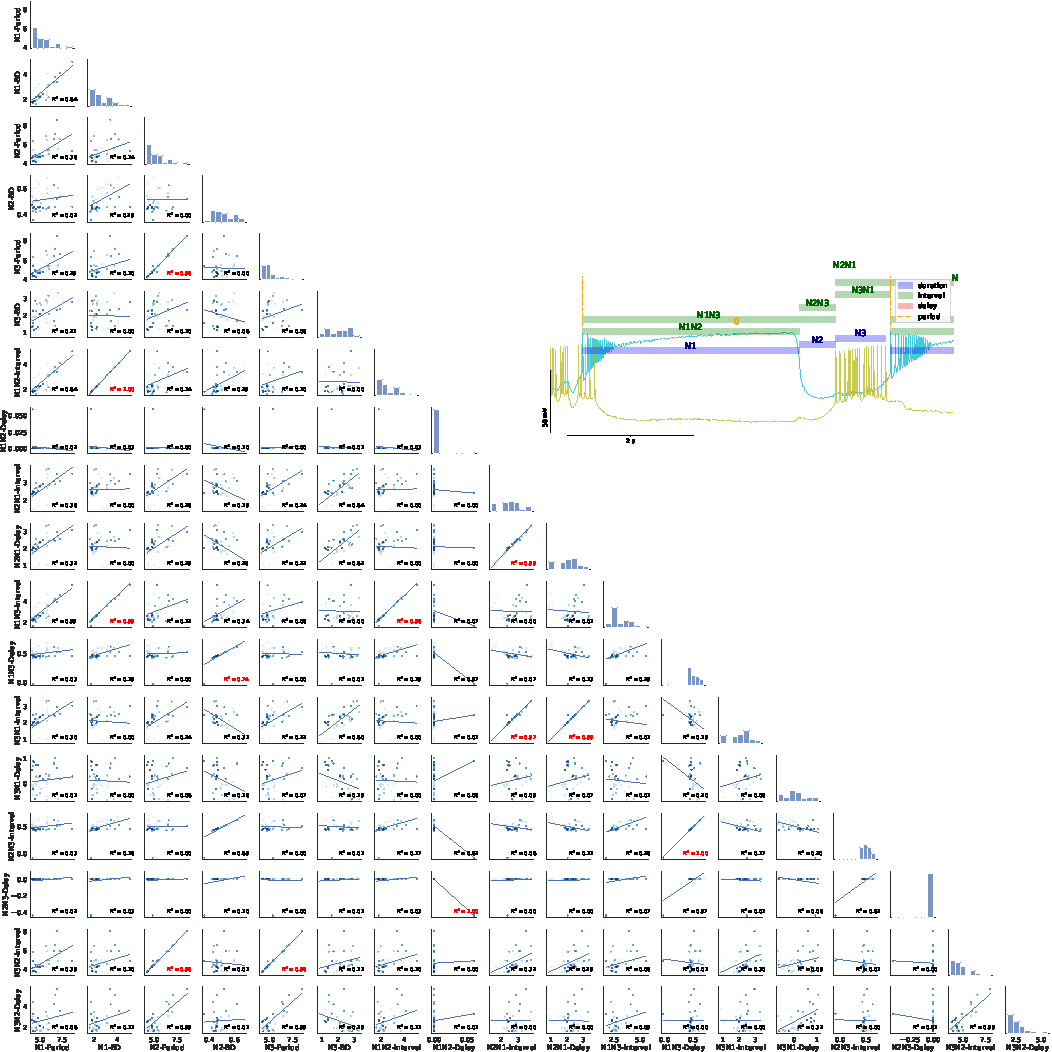
\includegraphics[width=0.9\textwidth]{./img/invariants/data/SUSSEX/CV1a_driven4/images/3phases/panel_with_pairplot.pdf}
%	\caption{\textbf{CV1a driven case 4}: Panel of intervals distribution and dynamical invariants for the three phases in the CPG under CV1a stimulation.}
%	\label{fig:cv1a 4 3phases pairplot}
%\end{figure}

\begin{figure}[htbp]
	\centering
	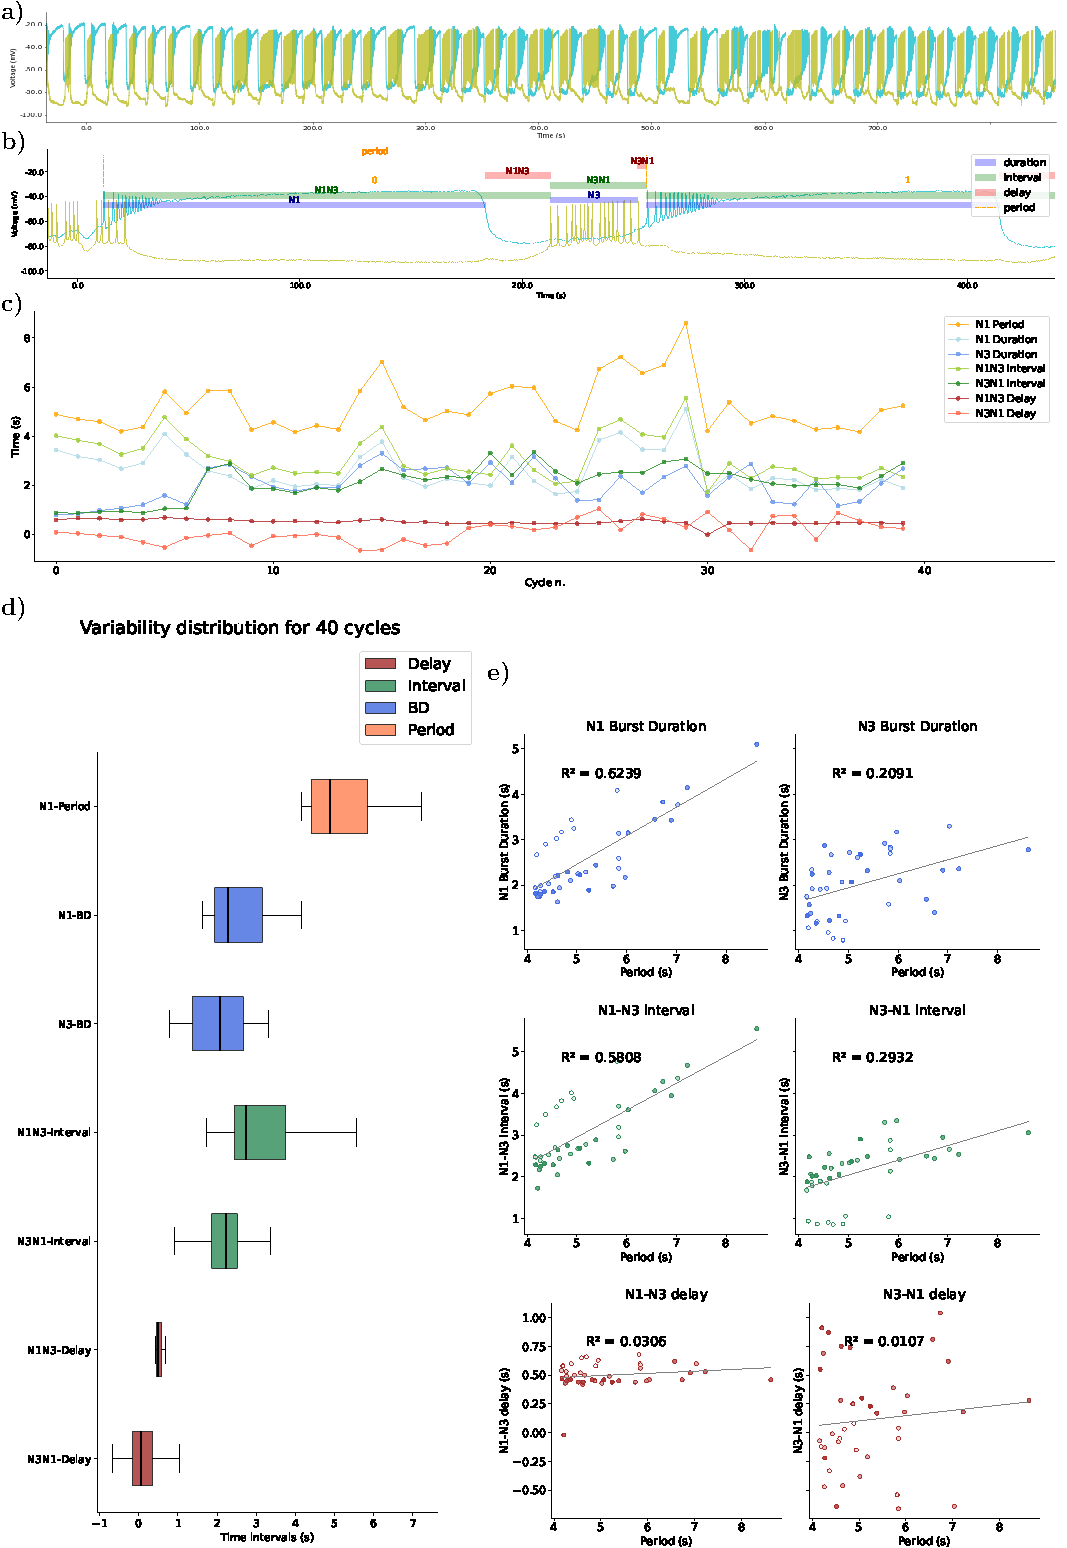
\includegraphics[width=0.9\textwidth]{./img/invariants/data/SUSSEX/CV1a_driven4/images/2phases/panel_with_intervals.pdf}
	\caption{\textbf{CV1a driven case4}: Panel of intervals distribution and dynamical invariants for the two phases in the CPG under CV1a stimulation.}
	\label{fig:cv1a 4 2phases}
\end{figure}

%\begin{figure}[htbp]
%	\centering
%	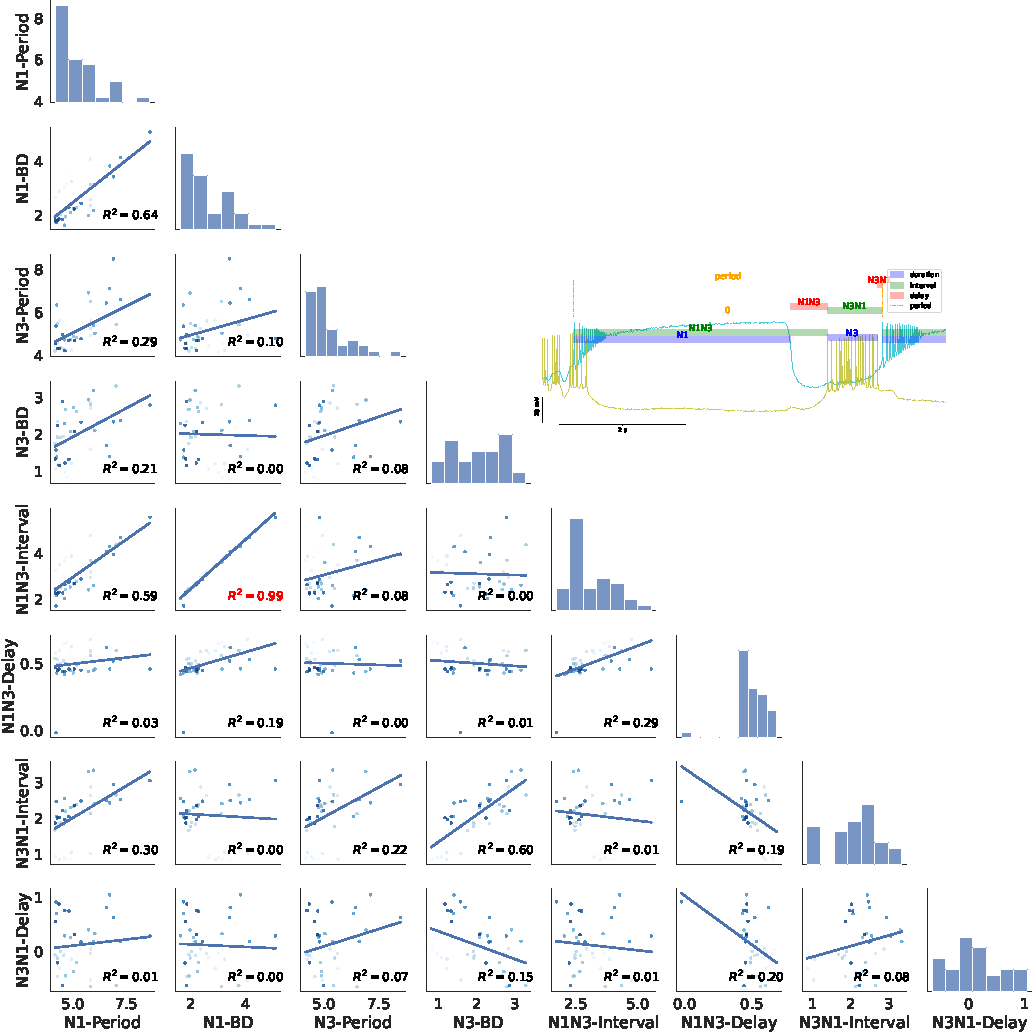
\includegraphics[width=0.9\textwidth]{./img/invariants/data/SUSSEX/CV1a_driven4/images/2phases/panel_with_pairplot.pdf}
%	\caption{\textbf{CV1a driven case4}: Panel of intervals distribution and dynamical invariants for the two phases in the CPG under CV1a stimulation.}
%	\label{fig:cv1a 4 2phases pairplot}
%\end{figure}



\begin{figure}[htbp]
	\centering
	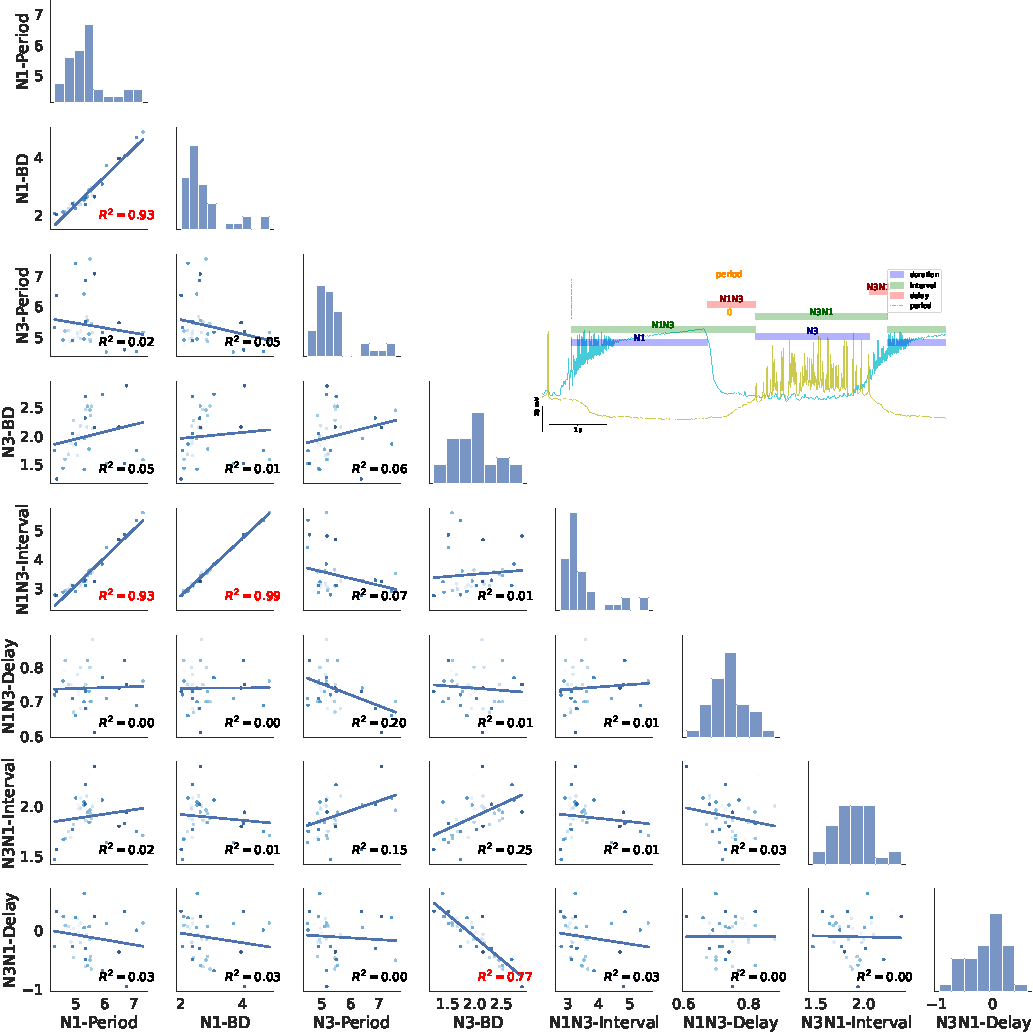
\includegraphics[width=0.48\textwidth]{./img/invariants/data/SUSSEX/CV1a_driven1/images/2phases/panel_with_pairplot.pdf}
	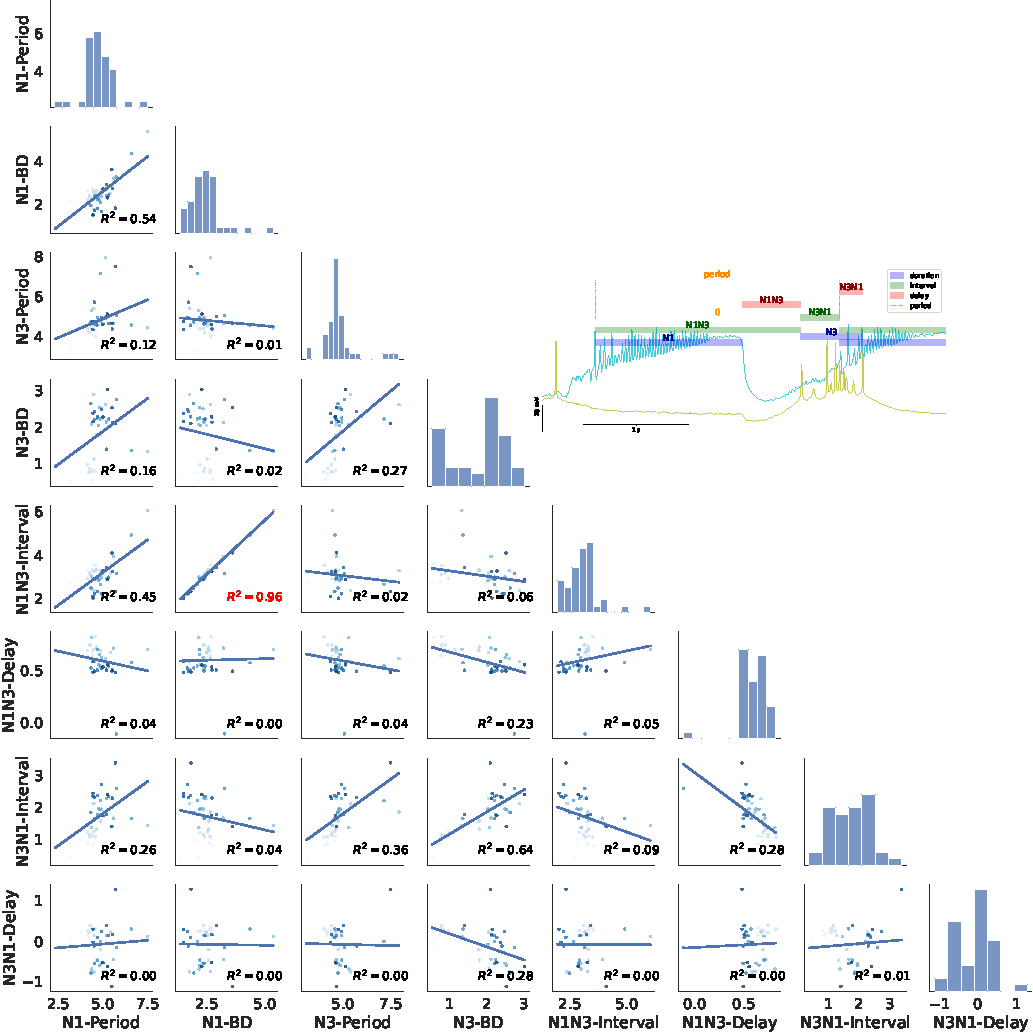
\includegraphics[width=0.48\textwidth]{./img/invariants/data/SUSSEX/CV1a_driven2/images/panel_with_pairplot.pdf}
	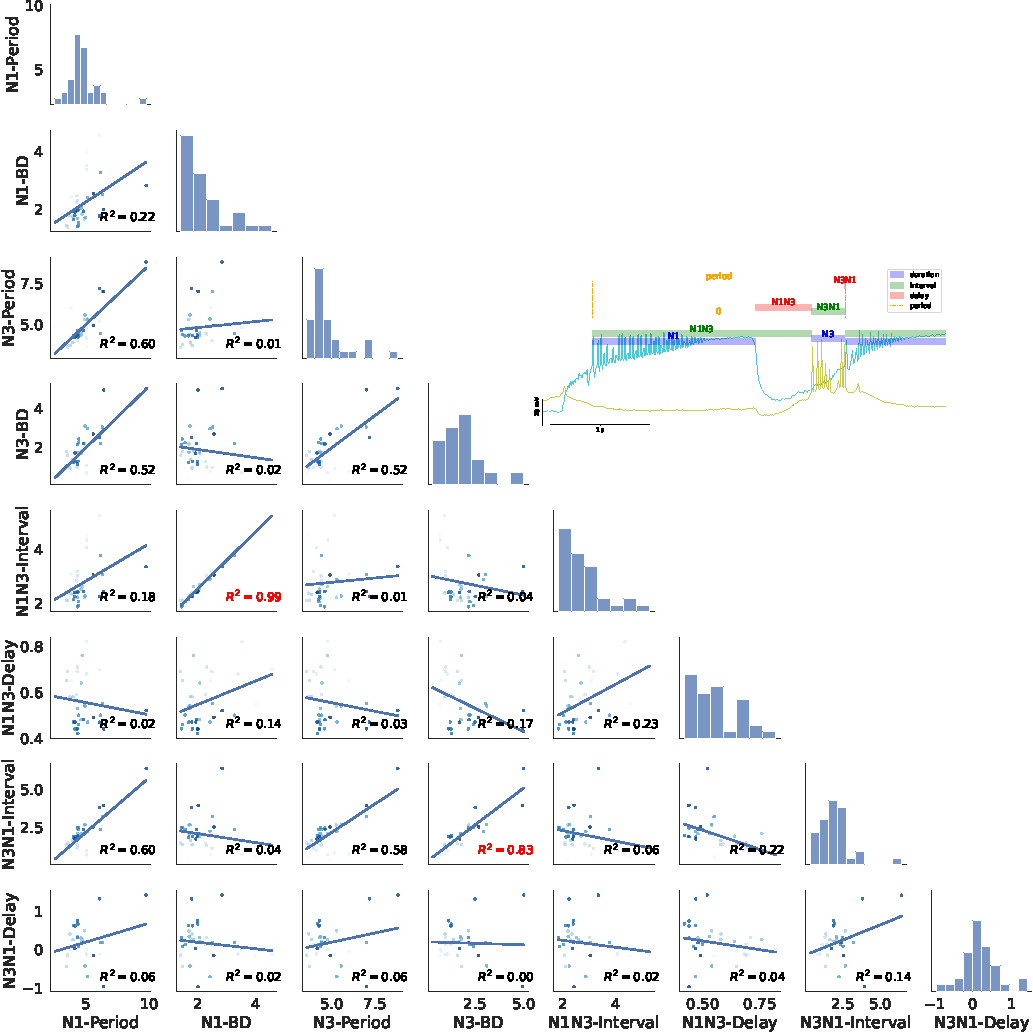
\includegraphics[width=0.48\textwidth]{./img/invariants/data/SUSSEX/CV1a_driven3/images/panel_with_pairplot.pdf}
	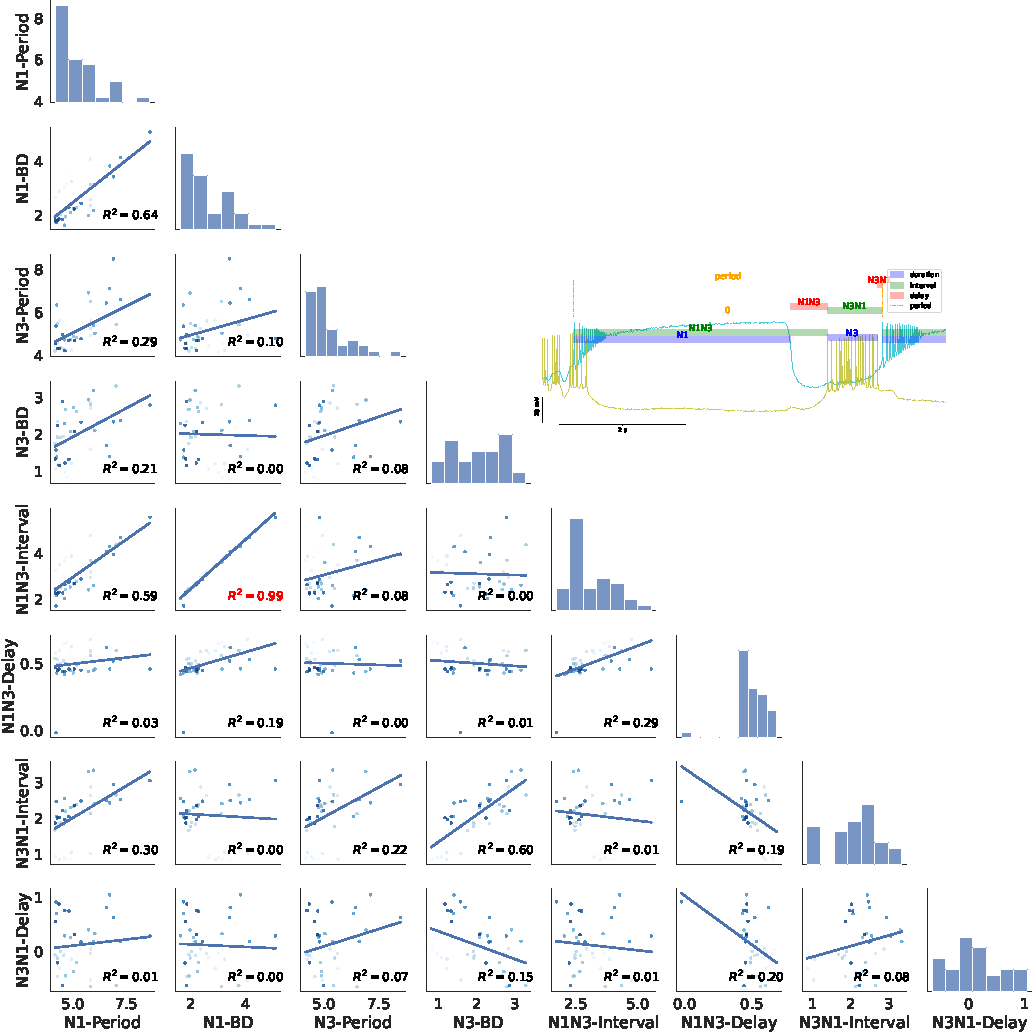
\includegraphics[width=0.48\textwidth]{./img/invariants/data/SUSSEX/CV1a_driven4/images/2phases/panel_with_pairplot.pdf}
	\caption{}
	\label{fig:cv1a pairplot comparison}
\end{figure}




\subsection{Summary}
\begin{figure}
	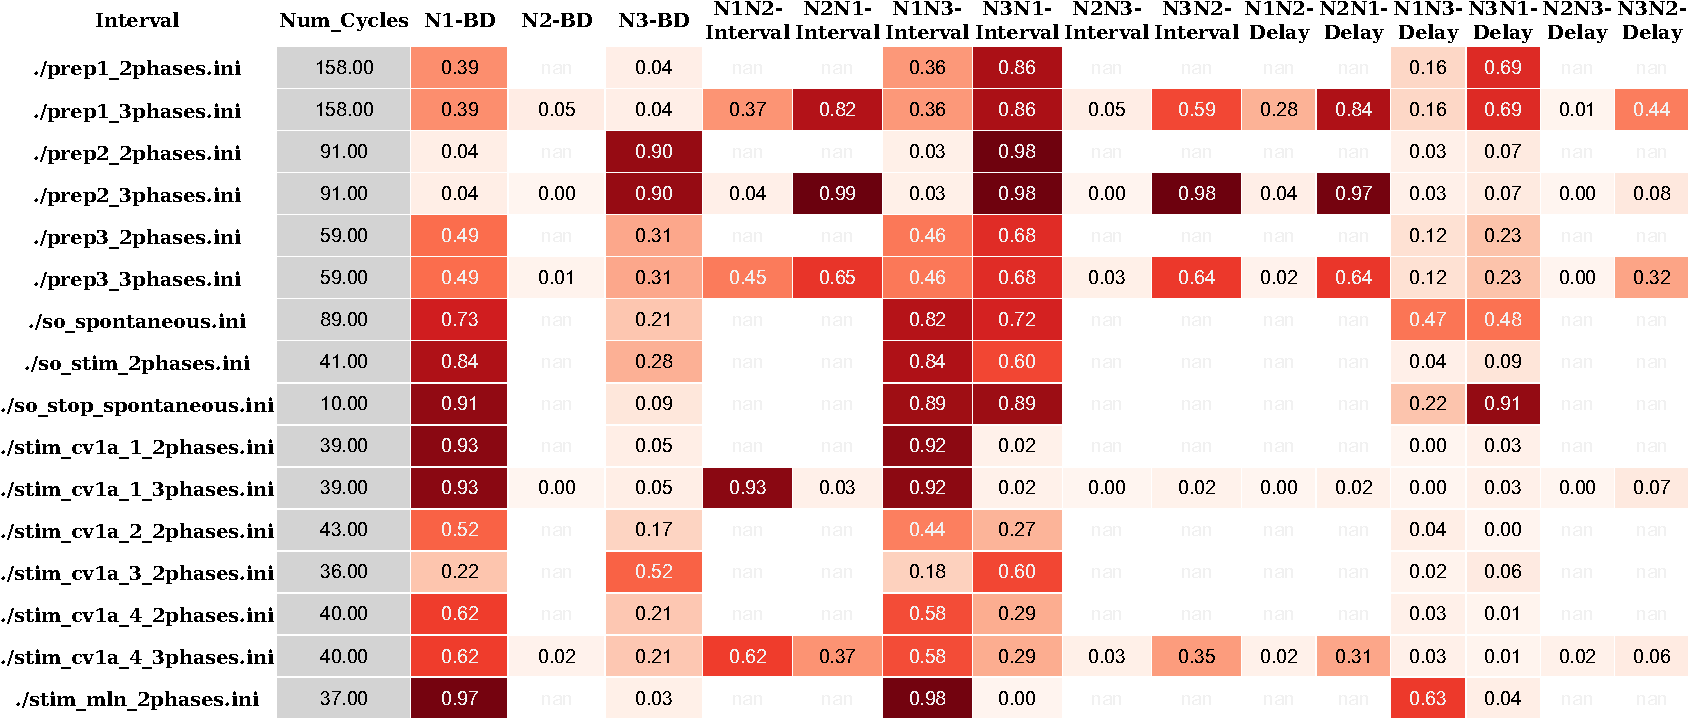
\includegraphics[width=\textwidth]{./img/invariants/styled_table_invariants_r-squared.pdf}
	\caption{Table of $R^2$ values for the linear regression between the period and each interval for all experimental recordings showed in this section.}
	\label{fig:R2 table}
\end{figure}

\begin{figure}
	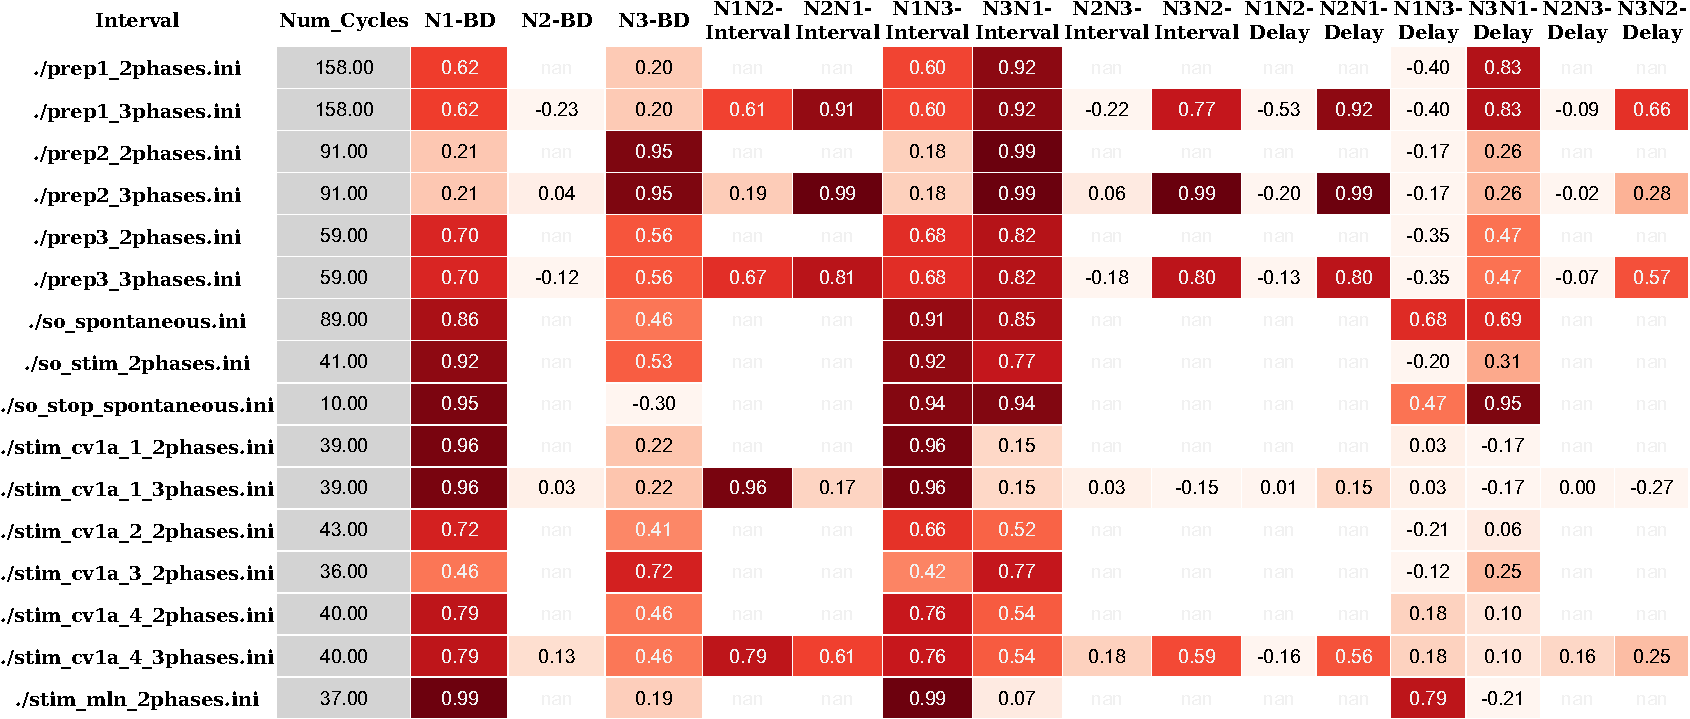
\includegraphics[width=\textwidth]{./img/invariants/styled_table_invariants_r-value.pdf}
	\caption{Table of $R$ values for the linear regression between the period and each interval for all experimental recordings showed in this section.}
	\label{fig:R table}
\end{figure}


\clearpage
\newpage
